\documentclass[12pt]{article}
\usepackage[english]{babel}
\usepackage{amsmath}
\usepackage{graphicx}
\usepackage{enumerate}
\usepackage{caption}
\usepackage{natbib}
\usepackage{subcaption}
\usepackage{amssymb}
\usepackage[colorinlistoftodos]{todonotes}
\usepackage{multicol}
\usepackage{authblk}
\usepackage{url} 
\usepackage{color}
\newcommand{\comment}[1]{{\color{blue} #1}}
\newcommand{\brittany}[1]{{\color{cyan} Brittany says: #1}}
\newcommand{\mike}[1]{{\color{orange} #1}}
% ... for graphics 
\graphicspath{{./}{figs/}}
% ... for easy and consistent referencing
\newcommand{\figref}[1]{Figure~\ref{#1}}
% ... mathematical symbols
\def\R{{\mathbb R}}

%\pdfminorversion=4
% NOTE: To produce blinded version, replace "0" with "1" below.
\newcommand{\blind}{0}

% DON'T change margins - should be 1 inch all around.
\addtolength{\oddsidemargin}{-.5in}%
\addtolength{\evensidemargin}{-.5in}%
\addtolength{\textwidth}{1in}%
\addtolength{\textheight}{1.3in}%
\addtolength{\topmargin}{-.8in}%


\begin{document}

%\bibliographystyle{natbib}

\def\spacingset#1{\renewcommand{\baselinestretch}%
{#1}\small\normalsize} \spacingset{1}


%%%%%%%%%%%%%%%%%%%%%%%%%%%%%%%%%%%%%%%%%%%%%%%%%%%%%%%%%%%%%%%%%%%%%%%%%%%%%%

\if0\blind
{
  \title{\bf Topological Hypothesis Tests for the Large-Scale Structure of the Universe}
  \author{Wu, Mike\thanks{
    The authors gratefully acknowledge \textit{please remember to list all relevant funding sources in the unblinded version}}\hspace{.2cm}\\
    Department of Computer Science, Yale University
    \and
    Cisewski, Jessi\\
    Department of Statistics, Yale University
    \and
    Fasy, Brittany T.\\
    Department of Computer Science, Montana State University
    \and
    Hellwing, Wojciech\\
    ICG, University of Portsmouth
    \and
    Lovell, Mark R.\\
    ITF, University of Amsterdam
    \and
    Rinaldo, Alessandro\\
    Department of Statistics, Carnegie Mellon University
    \and
    Wasserman, Larry\\
    Department of Statistics, Carnegie Mellon University
  }
  \maketitle
} \fi

\if1\blind
{
  \bigskip
  \bigskip
  \bigskip
  \begin{center}
    {\LARGE\bf Title}
\end{center}
  \medskip
} \fi

%%%%%%%%%%%%%%%%%%%%%%%%%%%%%%%%%%%%%%%%%%%%%%%%%%%%%%%
%% SECTION: ABSTRACT
%%%%%%%%%%%%%%%%%%%%%%%%%%%%%%%%%%%%%%%%%%%%%%%%%%%%%%%

\bigskip
\begin{abstract}
The large-scale structure (LSS) of the Universe is an intricate and spatially complex web.  In order to understand the physics of the Universe, theoretical and computational cosmologists develop large-scale simulations that allow for visualizing and analyzing the LSS under varying physical assumptions.  {\color{red}  add statement about WDM vs. CDM.}  However, rigorous comparisons and inference on such complicated structures can be problematic.  We present a framework for hypothesis testing of LSS using persistent homology.  The randomness in the data (due to measurement error or topological noise) is transferred to randomness in the topological
summaries, which provides an infrastructure for inference. These tests allow for statistical comparisons between complicated spatial data such as LSS in cosmology, but are also present in other areas of science.  We present several possible test statistics using persistence diagrams, carry-out a simulation study to investigate the suitableness of the proposed test statistics, and finally we apply the proposed inference frame work to {\color{red} WDM vs CDM}.
\end{abstract}

\noindent%
{\it Keywords:} persistent homology, voronoi, intensity, euler, silhouette, dark matter
\vfill

%%%%%%%%%%%%%%%%%%%%%%%%%%%%%%%%%%%%%%%%%%%%%%%%%%%%%%%
%% SECTION: INTRODUCTION
%%%%%%%%%%%%%%%%%%%%%%%%%%%%%%%%%%%%%%%%%%%%%%%%%%%%%%%

\newpage
\spacingset{1.45} % DON'T change the spacing!
\section{Introduction}
\label{sec:intro}

Rigorous comparisons of spatially complex web-like data such as the large-scale structure (LSS) of the Universe (see Figure~\ref{fig:introData}) is notoriously difficult due, in part, to the difficulty in capturing the randomness of geometric and topological structures.  However, these comparisons are important as it is becoming apparent that there is potentially information about cosmological parameters in the structure. We propose a framework for constructing  topological hypothesis tests using ideas from an emerging area of topological data analysis called persistent homology. Persistent homology offers a novel way to represent, visualize, and interpret complex data by extracting topological features, which can be used to infer properties of the underlying structures, and has already been used as an exploratory tool for some problems in astronomy (\cite{cisewski2014non, van2011alpha}) among other areas of science (\cite{bendich2014persistent, duong2012closed}).

The large-scale structure (LSS) of the Universe is an important example of a spatially complex structure that is often referred to as the \emph{Cosmic Web} \cite{bond1996filaments,springel2006large}.  The LSS of the Universe is a focus of manifold scientific research because its properties reveal information about the underlying physics and formation of our Universe {\color{red}  ADD CITATIONS}.  In order to study theoretical aspects of the formation and evolution of LSS, cosmologists develop large-scale simulations and can adjust the physical inputs and evaluate their effects on the LSS {\color{red} ADD CITATIONS of different simulations}.  One such input is related to the nature of dark matter.  The received position is that the Universe is made up of dark energy, dark matter (DM), and baryonic matter {\color{red} ADD CITATION}.  For an easy introduction to DM, see \cite[p. 61-63]{HilbeEtAl2014}.  

Though the generally accepted and best supported cosmological model assumes \emph{cold dark matter} (known as $\Lambda$CDM), there are some elements of disagreement with observations \cite{SchneiderEtAl2012}.  Furthermore, it has been demonstrated through cosmological simulations that the nature of DM affects the development and formation of LSS \cite{SchneiderEtAl2012}.  In Figure~\ref{fig:introData}, two realizations -- under the assumption of cold dark matter and warm dark matter -- from the EAGLE cosmological simulation {\color{red} ADD CITATION} are displayed.  Though there are similarities in shape of the densest regions (called \emph{filaments}, there are differences in the distribution of matter about the filaments.  

{\color{red} discuss simulation}
\begin{figure}[htp!]
  \centering
  \begin{subfigure}{.49\textwidth}
    \centering
    \caption{Eagle CDM Simulation}  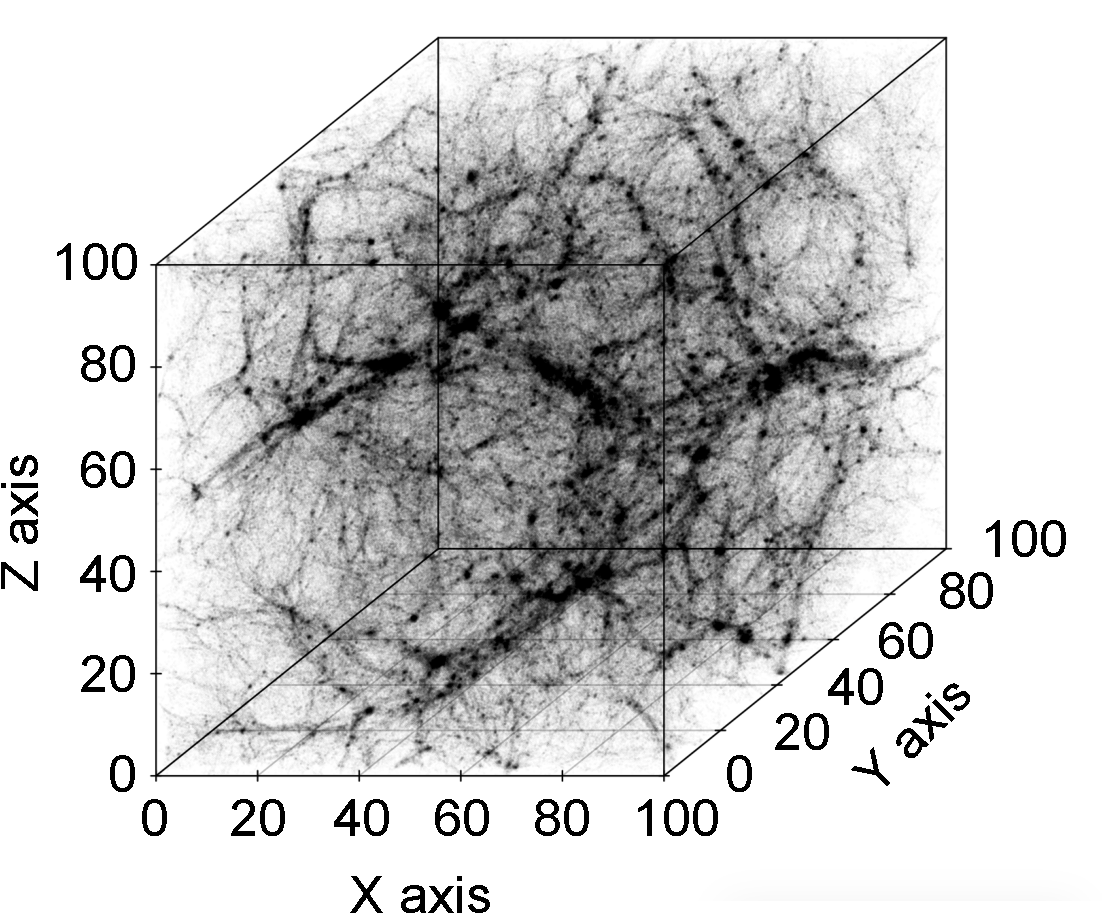
\includegraphics[width=\linewidth]{wdmfig.pdf}
    \label{fig:introDataCDM}
  \end{subfigure}
    \begin{subfigure}{.49\textwidth}
    \centering
    \caption{Eagle WDM Simulation}  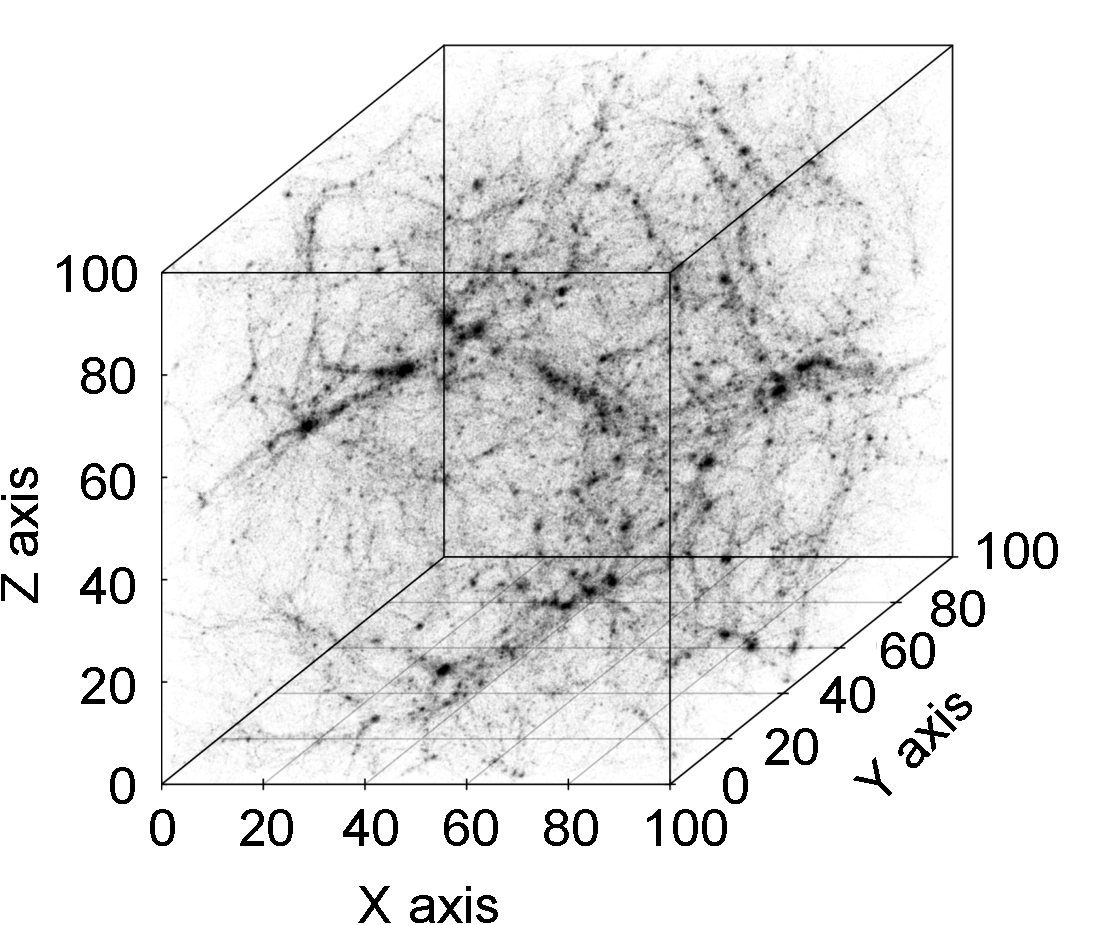
\includegraphics[width=\linewidth]{cdmfig.pdf}
    \label{fig:introDataWDM}
  \end{subfigure}
    \caption{EAGLE simulation under assumptions of (a) cold and (b) warm dark matter \cite{schaye2015eagle}.} 
    \label{fig:introData}
\end{figure}

The goal of the proposed topological hypothesis tests is to detect differences in the topology between these types structures using persistent homology.  In this paper, we move towards quantitatively detailing the topological and geometric differences between the LSS under respective assumptions of cold and warm dark matter.  We begin with an introduction to persistent homology followed by the proposed hypothesis testing framework.  Then we carry-out a simulation study to investigate the performance of the proposed test statistics.  Next we provide more background on LSS, and then apply the hypothesis tests to {\color{red} WDM vs. CDM}.  We end with concluding remarks.


%%%%%%%%%%%%%%%%%%%%%%%%%%%%%%%%%%%%%%%%%%%%%%%%%%%%%%%
%% SECTION: TOOLS FROM TDA
%%%%%%%%%%%%%%%%%%%%%%%%%%%%%%%%%%%%%%%%%%%%%%%%%%%%%%%

\section{Tools from TDA Useful for Studying LSS}
\label{sec:tda}
\brittany{Jessi, what exactly is the input data? a point cloud (where each point
    = a galaxy?) or a density
defined over a cube? I went with the point cloud here, but if this is not true,
I can rework this introduction.}

Homology is the study of the spatial structure of topological spaces (e.g., the
components of a subset of $\mathbb{R}^n$ and loops in $k$-nn graphs constructed
over point cloud data).  Persistent homology studies the spacial structure of a
parameterized family of topological spaces (e.g., keeping track of the so-called
births and deaths of homological features as a topological space changes in a
`nice' way).
%
The data set that we study is a cosmological point cloud, where each data point
represents a galaxy in the universe.  We then look at cubes in space and analyze
the distribution of galaxies within that cube. We may define a simplicial
complex directly on the data set, or we may compute a KDE from the input data.
The homological features mentioned above have cosmological interpretations in
dimensions zero, one, and two.  We discuss this briefly before going further
into the algebraic topology.

\paragraph{Clusters} 
A \emph{connected
component}, or zeroth dimensional homology feature, is a maximal subspace of a topological
space that cannot be covered by two disjoint open sets. In words, a connected
component is a `piece' of a topological space.  If our topological space is a
$k$-nn graph, then the components are clusters of data points.  In cosmology,
clusters of galaxies (or of stars or other cosmological matter) are an important
structure to understand, as the gravitational forces of these galaxies will
attract more cosmological matter to accumulate near the cluster.  Persistent
homology tracks the appearance of new connected components, and the merging of
two distinct components into one.

\paragraph{Filaments and Loops} \brittany{Write about this}

\paragraph{Cosmological Voids} \brittany{write about this}

\brittany{Jessi, is there a good source for the definitions of clusters, filaments, and voids?}

\subsection{Persistent Homology} 
Various methods can be used in order to transform a discrete point set into a
topological space. For example, points can be connected based on a distance (or
a distance-like structure as in \cite{chazal2011geometric}), or one can estimate
the density from which the points were sampled.  In the latter case, one would
look at a density function, such as a kernel density estimate (KDE) of a point
cloud and study the topological features of super-level sets of that density.
\brittany{add a citations for Hatcher/Munkres and Edels/Harer here}

\paragraph{Filtrations}
\brittany{define, the following is just a placeholder for now.}
To derive the persistent homology for $p$, let there exist a threshold
$r$, represented by a hyperplane that divides $p$ into two separate segments: a
super-level set, defined as $\{(x,y,z) \in p \textup{ s.t. } z \geq r \}$, and a
corresponding sub-level set $\{(x,y,z) \in p \textup{ s.t. } z < r \}$. $r$ is
initialized at $\infty$, at which the super-level set is empty and the sub-level
set contains all of $p$. The evolving spatial structure is represented by~$r$
approaching $-\infty$. The persistent homology would then track the connected
components ($\textup{H}_{0}$), loops ($\textup{H}_{1}$), and voids
($\textup{H}_{2}$) that appear and disappear in the super-level sets
$p^{-1}([r,\infty)]$ as $r$ ranges from $\infty$ to~$-\infty$. More
specifically, as~$r$ intersects $p$, the super-level set is no longer empty and
is instead, composed of disjoint peaks/local maxima.


\paragraph{Tracking Homology Generators}
\brittany{define PH, define feature -- this section is still in the works}
Each persistence point is plotted in the birth-death plane;
see~\figref{fig:homologyexample}(c) for an example.  Notice that for a
super-level set, all persistence points will be below the diagonal $x=y$.  A
diagonal point $(x,x)$ represents a feature that was born and died at the same
time $x$.  In order for the diagram to be stable, we include this diagonal with
infinite multiplicity \brittany{CITATION NEEDED}.  

The \emph{persistence} of a persistence point $(b,d)$ is the length of the
interval of persistence parameters that support that feature: $b-d$.  In the
persistence diagram, the distance from $(b,d)$ to the diagonal is proportional
to this value; in fact, the (Euclidean) distance to the diagonal is
$1/\sqrt{2}(b-d)$. Often, the persistence of a feature is indicative of the
significance of the feature, which means that points close to the diagonal are
indistinguishable from noise.

\begin{figure}
  \begin{subfigure}{.27\linewidth}
    \centering
    \caption{}  
        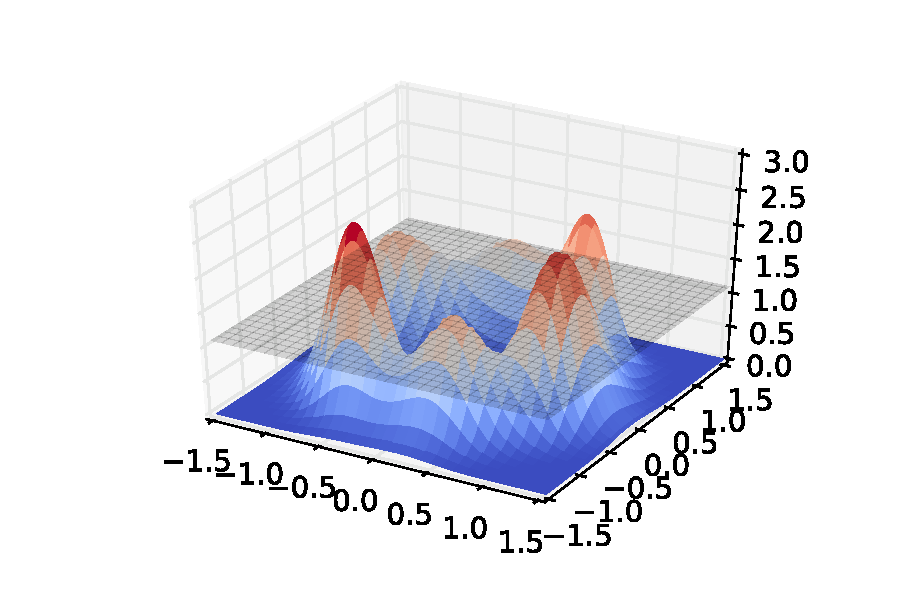
\includegraphics[width=\linewidth]{tmp2.pdf}
    \label{fig:example_3d}
  \end{subfigure}
    \begin{subfigure}{.25\linewidth}
    \centering
    \caption{}  
        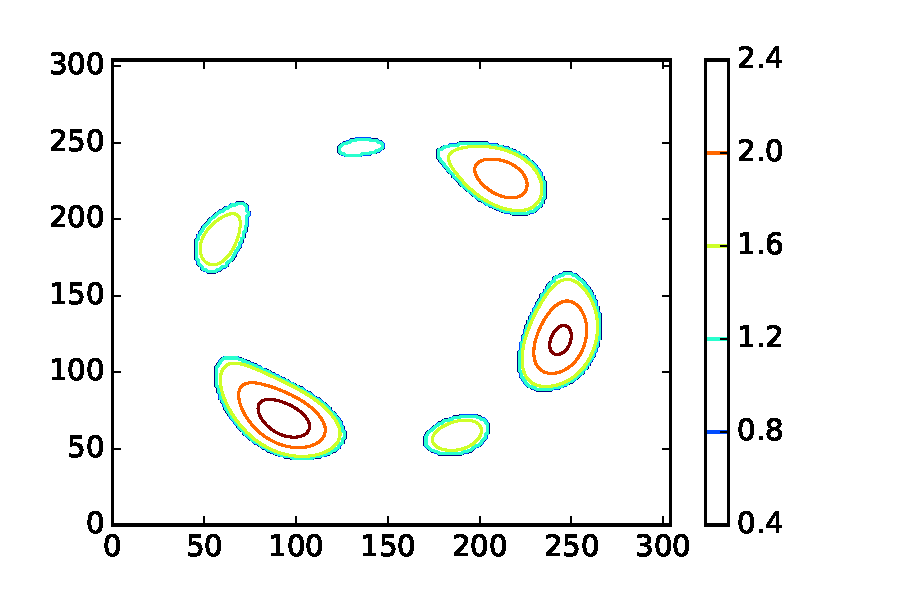
\includegraphics[width=\linewidth]{tmp4.pdf}
    \label{fig:example_contour1}
  \end{subfigure}
    \begin{subfigure}{.25\linewidth}
    \centering
    \caption{}  
        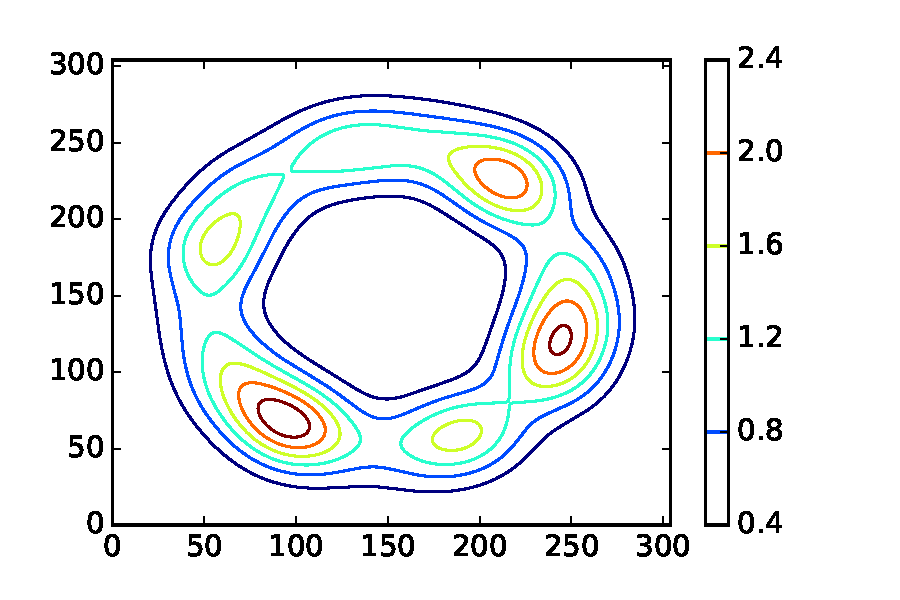
\includegraphics[width=\linewidth]{tmp3.pdf}
    \label{fig:example_contour2}
  \end{subfigure}
    \begin{subfigure}{.20\linewidth}
    \centering
    \caption{}  
        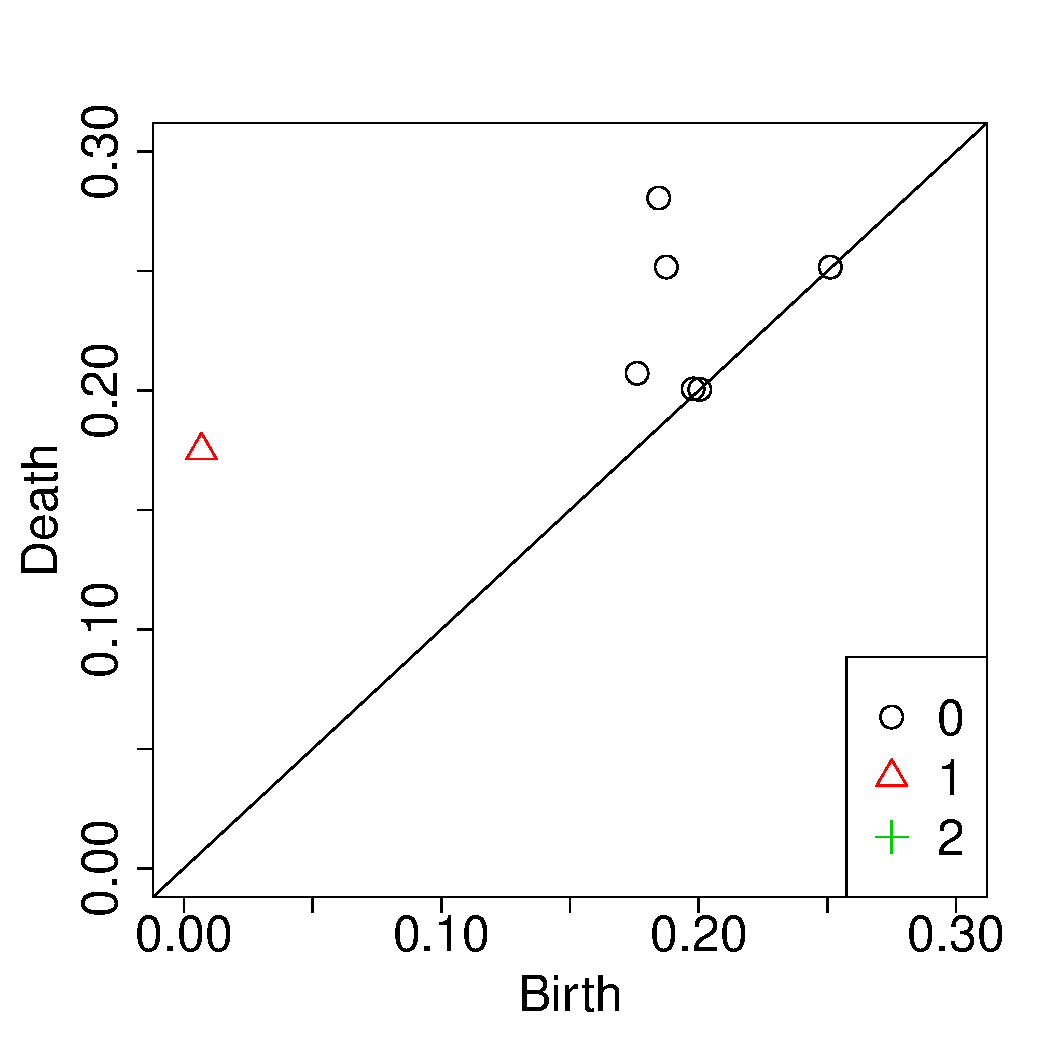
\includegraphics[width=\linewidth]{tmp5.pdf}
    \label{fig:example_pd}
  \end{subfigure}
  \caption{ We illustrate persistent homology with a two-dimensional example. The density in (a) shows 3 steep peaks and 3 shallow peaks  distributed around a uniform circle. In light gray, we see the hyperplane, shown (b) as $t=1.0$. (b) and (c) plot the super-level sets $\widehat{p}^{-1}[1.10,\infty)$ and $\widehat{p}^{-1}[0.10,\infty)$ respectively. Notice as the threshold is decreased, the contour more clearly defines a loop-like structure. In (d), we see the  persistence diagram for the super-level set filtration of $\widehat{p}$. We highlight the upper left quadrant based at $(0.18, 0.02)$, which contains a one-dimensional persistence point. This corresponds to the loop shown in (c). The remaining 0-dimensional homologies represent the connected components from each of 6 peaks.} % end caption
    \label{fig:homologyexample}
\end{figure}

\paragraph{An Example}
In order to illustrate persistent homology, we step down a dimension from cubes in $\R^3$ to squares in $\R^2$. In \figref{fig:homologyexample}, we see how persistent homology captures
the evolving super-level sets of a KDE $\widehat{p} \colon [-2,2]^2 \to \R$.  The density plot in \figref{fig:homologyexample} was created using 6 Gaussian peaks distributed along a uniform circle in the $<x,y>$ plane. As the persistence parameter $t$, shown as a hyperplane, decreases from $\infty$ to $-\infty$, various events occur in the
super-level sets $\widehat{p}^{-1}[t,\infty)$: a new component can appear (zero-dimensional birth), two distinct components can merge (zero-dimensional death), a loop can appear (one-dimensional birth), and two loops can become homologous (one-dimensional death).  These birth and death events are paired and plotted in the persistence diagram.
%
In the persistence diagram of \figref{fig:homologyexample}(a), we see exactly 6 zero-dimensional persistence points (denoted by black circles), one for each of the Gaussian peaks, and a single
one-dimensional persistence points (denoted by red triangles), representing the circle on which the modes are located and is captured
in \figref{fig:homologyexample}(c).

The upper-left quadrant based at a point $(x,x)$ will contain all persistence points that are born before $x$ and die at or after $x$; that is, the persistence points in this quadrant are in one-to-one correspondence with generators of $p^{-1}(x,\infty)$.  In this way, the homology of each super-level set can be read off of the persistence diagram.  
\brittany{todo:
continue here (update for new example)}

\subsection{Derivatives of Persistence Diagrams}
\brittany{sentence here}
\paragraph{Landscapes and Silhouettes}
Weighted silhouette functions are formed by weighting a particular functional summary of persistence diagrams called \emph{landscape functions} \cite{bubenik2015statistical}.  Details and theoretical properties of landscapes and silhouettes are provided in \cite{chazal2014stochastic}.

Landscape functions are defined as follows.  Let the finite birth and death intervals of a persistence diagram with $n_h$ points, for homology dimension $h = 0, 1, 2, \ldots$, be defined as $\{(b_{hi},d_{hi})\}_{i = 1}^{n_h}$.  Next consider rotating the persistence diagram such that a given point is $p_{hi} = \left(\frac{b_{hi}+d_{hi}}{2}, \frac{d_{hi}-b_{hi}}{2}\right) \in D_h, \quad i = 1, \ldots, n_h$.  Equilateral triangles are formed from each $p_{hi}$ to the base as

\begin{equation*}
\Lambda_{p_{hi}}(t) =
  \begin{cases}
    t - b_{hi}  & \quad t \in [b_{hi}, \frac{d_{hi}+b_{hi}}{2}]\\
    d_{hi} - t  & \quad t \in [\frac{d_{hi}+b_{hi}}{2}, d_{hi}]\\
    0  & \quad \text{ otherwise}\\
  \end{cases}
\end{equation*}
where $t \in [t_{\min}, t_{\max}]$. 

For a given $h$, the persistence landscape is then defined as the following collection of functions

\begin{equation*}
\lambda_{D_h}(k, t) = \underset{p_{hi}\in D_h}{\text{kmax }} \Lambda_{p_{hi}}(t), \quad t \in [t_{\min}, t_{\max}], k = 1, \ldots, n_h
\end{equation*}
where kmax is the kth largest value in $D_h$.  An example of a landscape function is displayed in Figure~\ref{fig:landscape}.

\begin{center}
\begin{figure}[htp!]
  \centering
  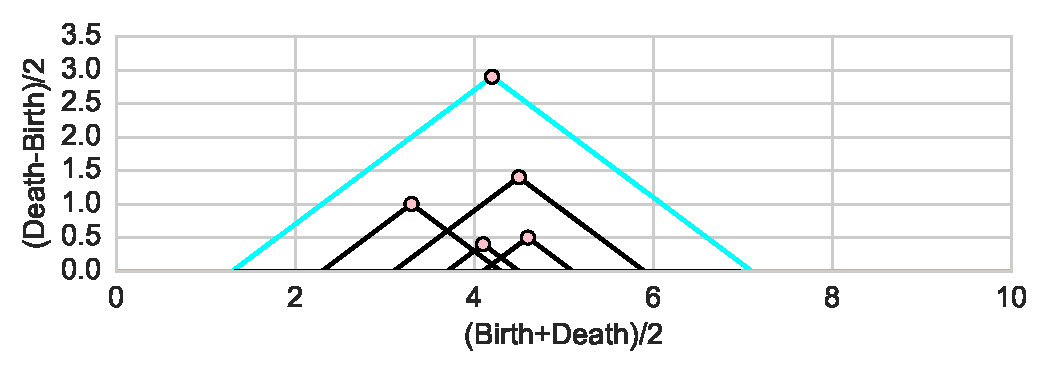
\includegraphics[width=0.5\linewidth]{example_landscape.pdf}
    \caption{ The shaded circles in pink represent the point coordinates in a persistence diagram $D$. The landscape $\lambda(k, \cdot)$ is the $k$-th largest of the arrangement of the graphs of $\left \{ \Lambda_{p} \right \}$. In particular, the cyan curve is the landscape $\lambda(1, \cdot)$.}
    \label{fig:landscape}
\end{figure}
\end{center}

Rather than working with each $k$ of $\lambda_{D_h}(k, t)$ individually, silhouettes provide a way of combining the information in the collection of landscape functions.  Silhouettes are weighted averages of the individual functions for homology dimension $h$ defined~as

\begin{equation*}
\phi_h(t) = \frac{\sum_{i = 1}^mw_{hi}\Lambda_{hi}(t)}{\sum_{i = 1}^mw_{hi}}
\end{equation*}
where the weights $w_i$ can be defined to give more emphasis or less emphasis to features with longer lifetimes.  As suggested in \cite{chazal2014stochastic}, we use $w_{hi} = |d_{hi} - b_{hi}|^p$, where $p$ is a tuning parameter that needs to be selected.

\paragraph{Euler Characteristic Function}
The Euler characteristic is a topological invariant and defined as an alternating sum of Betti numbers, where~$N$ is the number of dimensions: $\chi = \beta_{0} - \beta_{1} + \beta_{2} - \beta_{3} + ... \pm \beta_N = \sum_{i=0}^{N} (-1)^{i} \beta_{i}$,
where $\beta_{i}$ represents the $i$-th Betti number, or the rank of the $i$-th homology group. When analyzing persistence diagrams of LSS, since there exist only three dimensions of data, the only non-trivial homology groups will be in dimensions 0, 1, and 2. Given the Betti numbers $\beta_{0}$, $\beta_{1}$, and $\beta_{2}$, the Euler characteristic equation simplifies to:

\[ \chi = \beta_{0} - \beta_{1} + \beta_{2} \]

The topological space is parameterized by the threshold, $t$ (ranging from $t_{\min}$ to $t_{\max}$), defining the upper-level sets. The homology groups (and hence Betti numbers) can be computed using $H_{0}$, $H_{1}$, and $H_{2}$ at each threshold $t$. Plotting the Euler characteristic against $t$, we obtain the Euler Characteristic function, $\chi(t)$. 

%%%%%%%%%%%%%%%%%%%%%%%%%%%%%%%%%%%%%%%%%%%%%%%%%%%%%%%
%% SECTION: METHODS
%%%%%%%%%%%%%%%%%%%%%%%%%%%%%%%%%%%%%%%%%%%%%%%%%%%%%%%

\section{Methods}
\label{sec:methods}
Given single point cloud of data, persistent homology can be used to summarize its topological information in a persistence diagram.  Though a persistence diagram can be interesting on its own, it would be useful to have a way to compare and test differences in topological structure.  Next, we describe several frameworks for using persistence diagrams in two-sample hypothesis tests.  

\begin{sloppypar}
Suppose we have two sets of persistence diagrams, $\{\mathcal 
P_1^{(1)}, \ldots, \mathcal P_n^{(1)}\}$ and $\{\mathcal P_1^{(2)}, \ldots, 
\mathcal P_m^{(2)}\}$.  These samples can be used to test $H_0: \mathcal 
P^{(1)} = \mathcal P^{(2)}$ vs. $H_2: \mathcal P^{(1)} \neq \mathcal P^{(2)}$, 
where $\mathcal P^{(1)}$ and $\mathcal P^{(2)}$ are the true underlying 
distributions of persistence diagrams for group 1 and 2, respectively. We would like the framework to test the hypothesis that the two samples are drawn from a population with the 
same random topology. However, we note that without incorporating a scaling adjustment on the space of the data or the space of the diagrams, geometrical differences can also 
lead to a rejection of the null hypothesis.  This is discussed in more detail in Section~\ref{sec:standardize}. 
\end{sloppypar}

Given two samples of persistence diagrams, there are a number of possible ways to derive test statistics.  We select four possible approaches with 9 individual tests. The first approach is based on functional summaries derived from the sampled persistence diagrams:  
Euler characteristic function (EC), Silhouette function (Sil), and a 
Silhouette-Euler characteristic function (SilEC).  Each observed dataset will 
have a corresponding functional summary.  A p-value can be derived from 
a two-sample T-test based on the integral of the absolute value of the 
functional summaries.  The next two approaches use variations on smoothed persistence diagrams called \emph{intensity functions} \cite{chen2015statistical} with p-values derived from a two-sample kernel test \cite{gretton2012kernel} and an asymptotic argument through permutation (KC, WKC, PI). Additionally, we consider a test using the two-point correlation function (CORR) in order to have a comparison with a summary capturing the spatial behavior of the LSS. Similar to the functional summaries above, p-values for the CORR test will be carried out with a T-test based on the integral of the absolute value of the correlation function. The proposed test statistics are discussed in more detail below.

% Given any persistence diagram $x$ extracted from a point cloud, $x$ represents a sample from some latent distribution $\chi$. For example, given a simulation of the Megaparsec cosmic mass, the $(x, y, z)$ points are discrete samples from the continuous, observable Universe, which represents the true distribution. Using that definition, suppose there are two persistence diagrams, $x$ and $y$, each produced from a separate point cloud. Given that $x \sim \chi$, and $y \sim \gamma$, where $\chi$ and $\gamma$ represent the true distributions, an interesting question is whether $\chi$ and $\gamma$ are identical to some error $\epsilon$. In other words, are the samples $x$ and $y$ sampled from the same latent distribution? One might consider the following hypothesis test, where $H_{0}$ is the null and $H_{A}$ is the alternative.

% \[ H_{0} : \chi = \gamma \]
% \[ H_{A} : \chi \neq \gamma \]

% However, given that the parameters of the distributions $chi$ and $\gamma$ are unknown, one cannot directly compare them. Instead, one much infer the relationship between $chi$ and $gamma$ by comparing the diagrams sampled from $\chi$ and $\gamma$ respectively. Given $n$ samples, a hypothesis test should be designed to compare $\{ x_{1}, ..., x_{n} \sim \chi \}$ and $\{ y_{1}, ..., y_{n} \sim \gamma \}$. However, comparing two persistence diagrams, $x$ and $y$, is non-trivial. Naive distance calculations, like bottleneck or Wasserstein, are easily perturbed by randomness and noise, and are computationally expensive. Instead, we propose to further summarize a persistence diagram by a test statistic. To find such a test statistic, we must define a function $f_{T}$ that takes an input $x$ and produces a statistic $T_{x}$, $f_{T}(x) = T_{x}$. Provided such a function exists, using the further summarized statistics, we can test the hypothesis that two persistence diagrams, $x$ and $y$ are sampled from the same latent distribution with the following framework:

% \[ H_{0} : f_{T}(x) = f_{T}(y) \]
% \[ H_{A} : f_{T}(x) \neq f_{T}(y) \]

% One main contribution of this paper is studying the effectiveness of different functions $f_{T}$ when the true topological relationship between $x$ and $y$ are known. The best functions $f_{T}$ are then used to analyze a data set in which the topological relationships is unknown. We now proceed to describe different methods for defining $f_{T}$ for hypothesis testing in the setting of large-scale structure (LSS). 

Among the nine variations to test statistics considered (EC, Sil, SilEC, KC, WKC, PI, and CORR), we are seeking the summary that best captures differences in distributions of persistence diagrams produced from structures like the LSS of the Universe.  

\paragraph{Euler Characteristic Test (EC)}
To use the Euler characteristic (EC) function, $\chi(t)$, in a hypothesis testing framework, the absolute value of the EC function is integrated with respect to the threshold $t$ to produce an Euler test statistic, $\widehat{EC}$:

\begin{equation*}
\widehat{EC} = \int_{t_{\min}}^{t_{\max}} | \chi(t) | \textup{ d}t.
\end{equation*}

Given the Euler statistics for two sets of persistence diagrams (where a set contains persistence diagrams drawn from the same topological distribution), a T-test is used to calculate a p-value for the null hypothesis that the two sets of persistence diagrams are sampled from the same distribution. 

\begin{figure}[htbp]
   \centering 
  \begin{subfigure}{.24\textwidth}
    \centering
        \caption{Point Cloud}       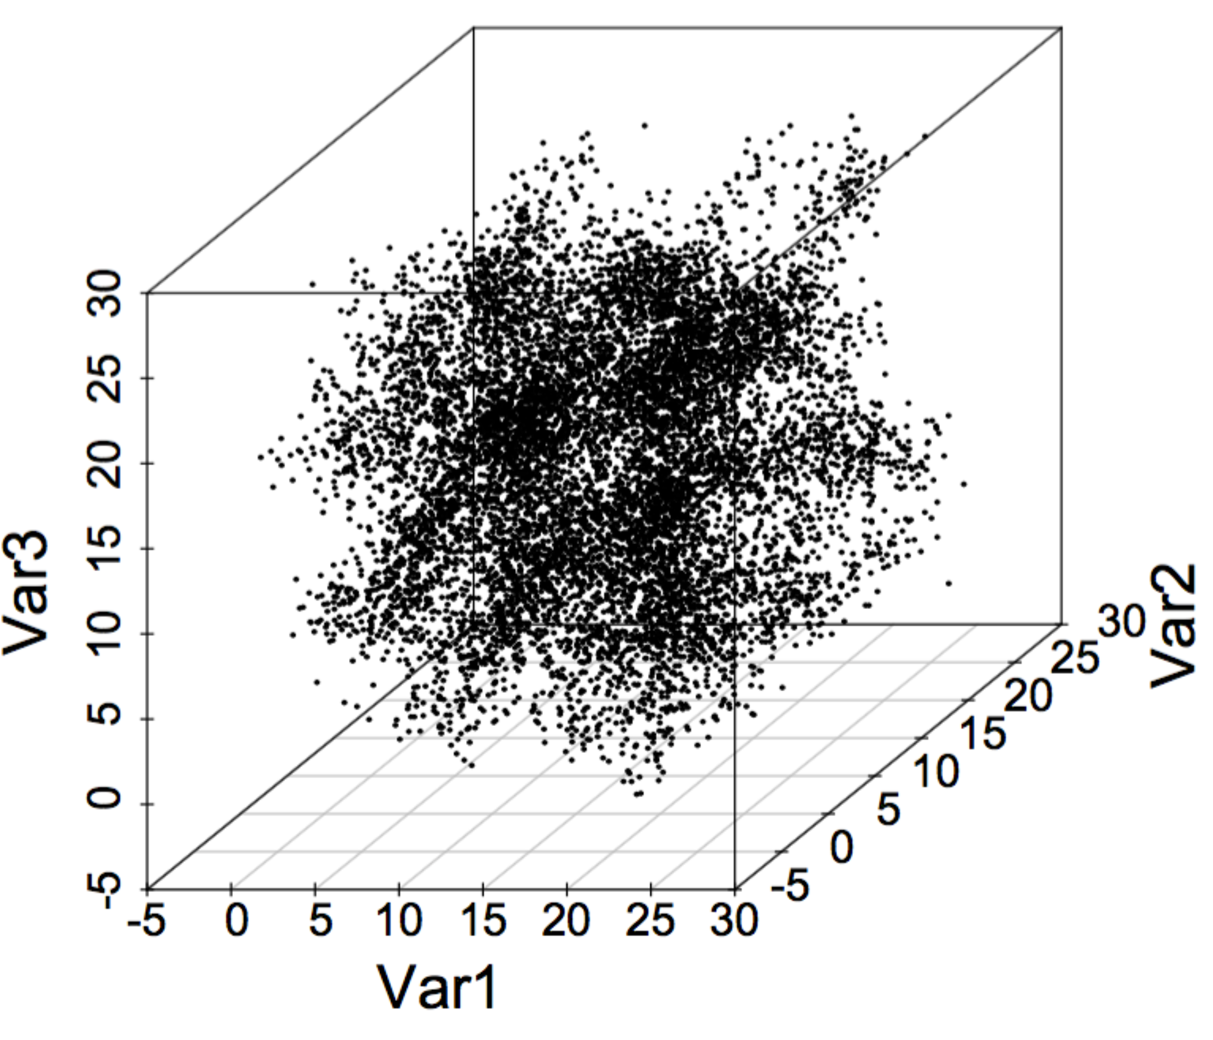
\includegraphics[width=\linewidth]{test_pics_1.pdf}
    \label{fig:examplestest1}
  \end{subfigure}
    \begin{subfigure}{.24\textwidth}
    \centering
        \caption{PD}  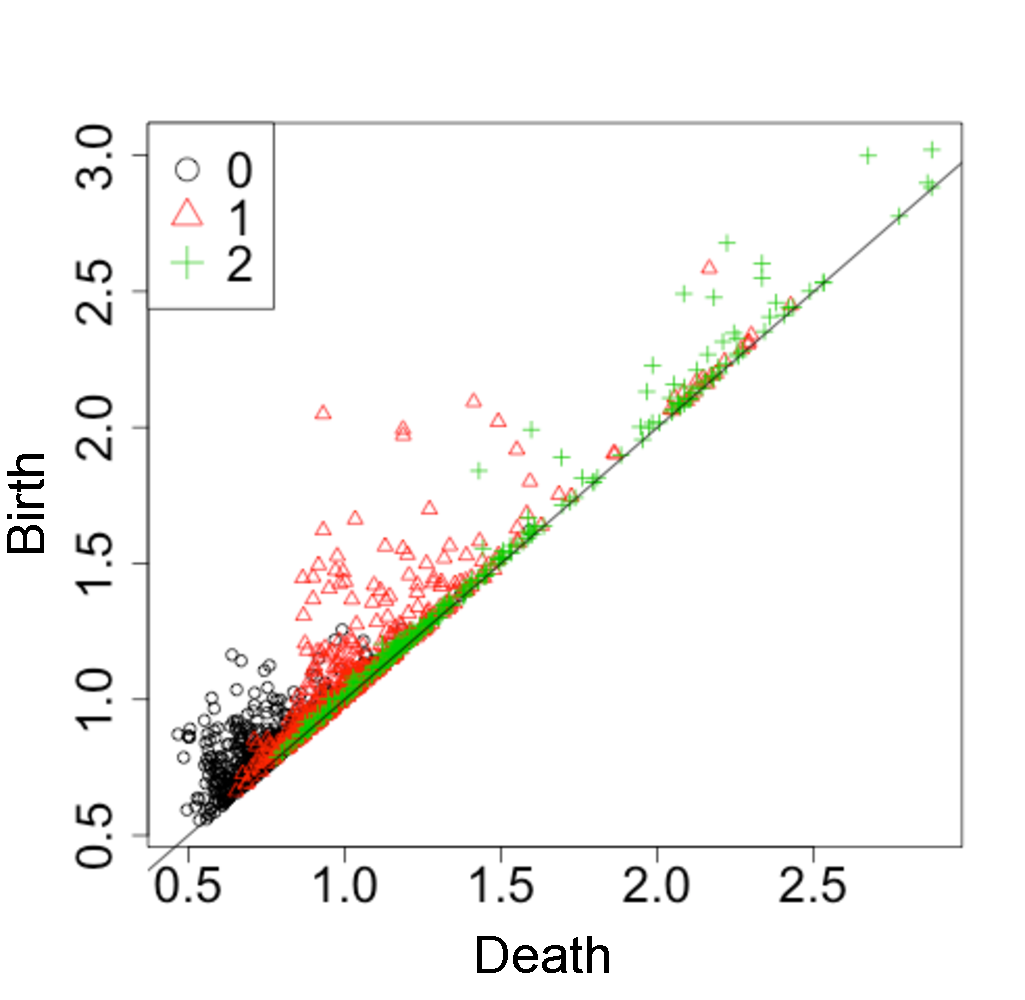
\includegraphics[width=\linewidth]{test_pics_2.pdf}
    \label{fig:examplestest2}
  \end{subfigure}
    \begin{subfigure}{.24\textwidth}
    \centering
        \caption{Euler Char.}   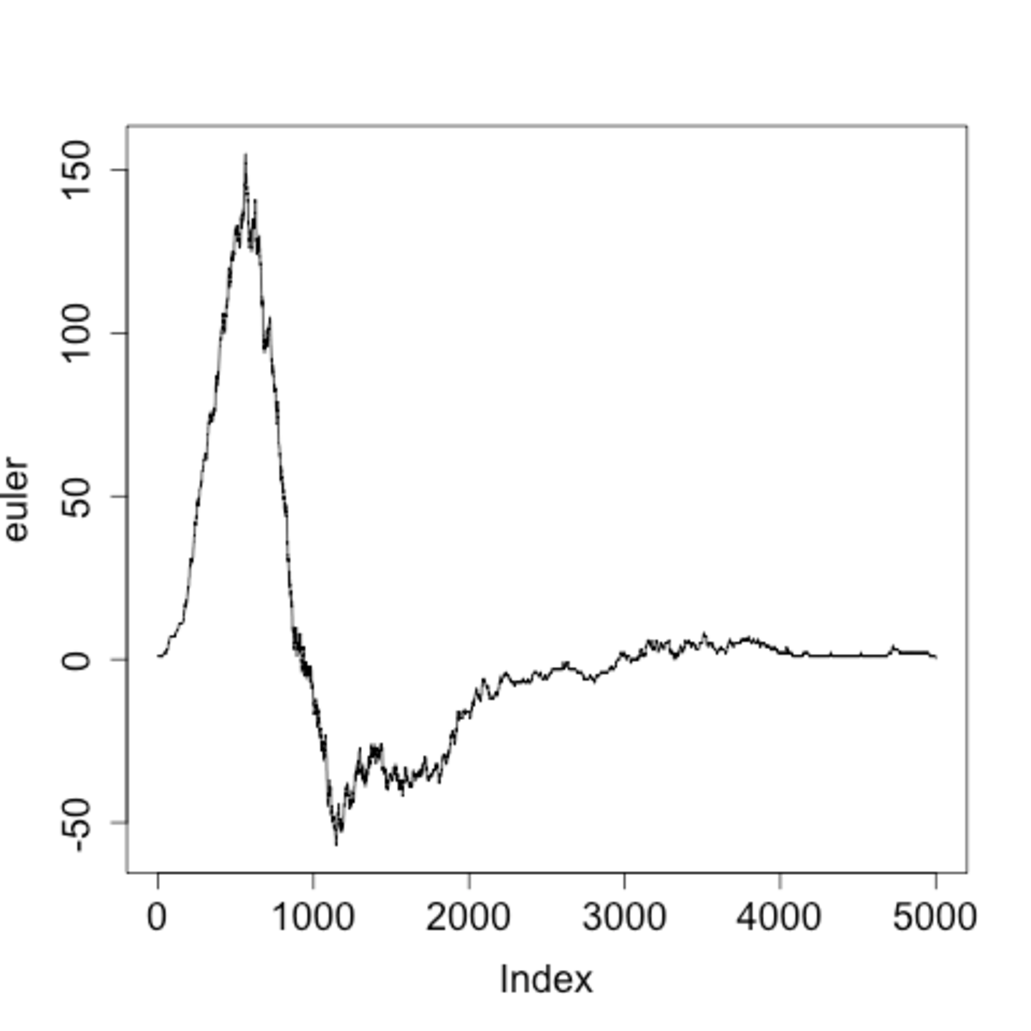
\includegraphics[width=\linewidth]{test_pics_3.pdf}
    \label{fig:examplestest3}
  \end{subfigure}
    \begin{subfigure}{.24\textwidth}
    \centering
        \caption{Sil. Function}       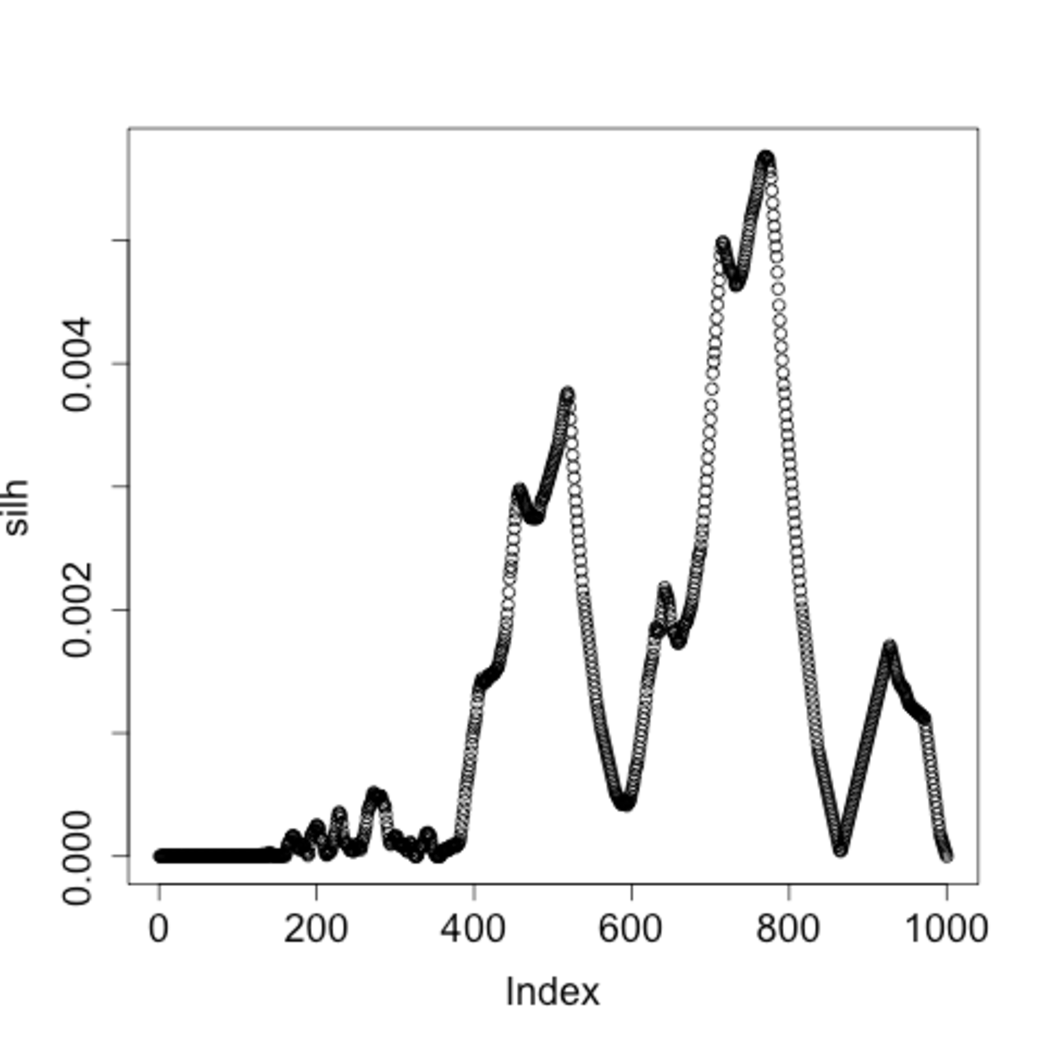
\includegraphics[width=\linewidth]{test_pics_4.pdf}
    \label{fig:examplestest4}
  \end{subfigure}
    \begin{subfigure}{.24\textwidth}
    \centering
        \caption{Kernel Contour}  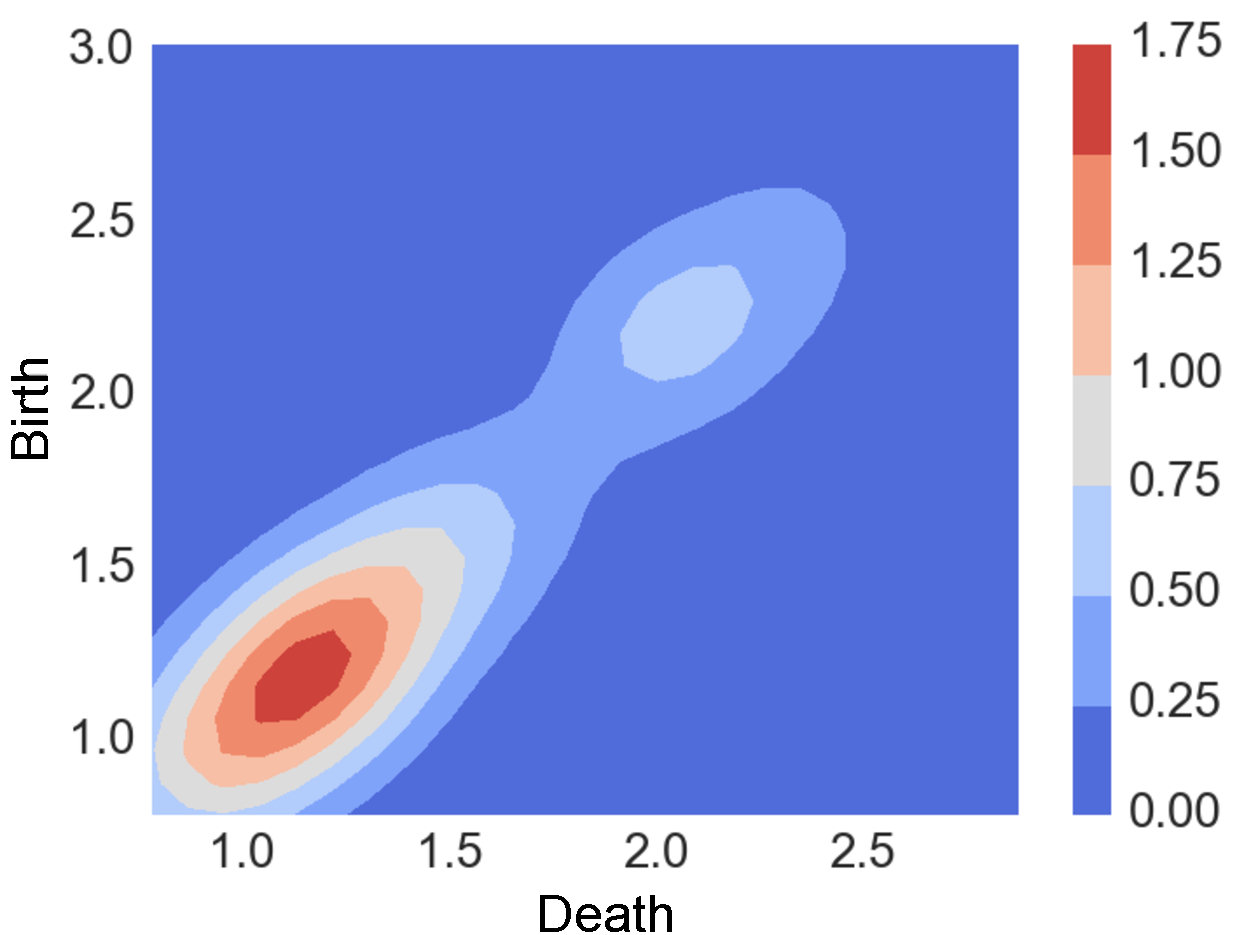
\includegraphics[width=\linewidth]{test_pics_5.pdf}
    \label{fig:examplestest5}
  \end{subfigure}
    \begin{subfigure}{.24\textwidth}
    \centering
        \caption{Corr. Function}  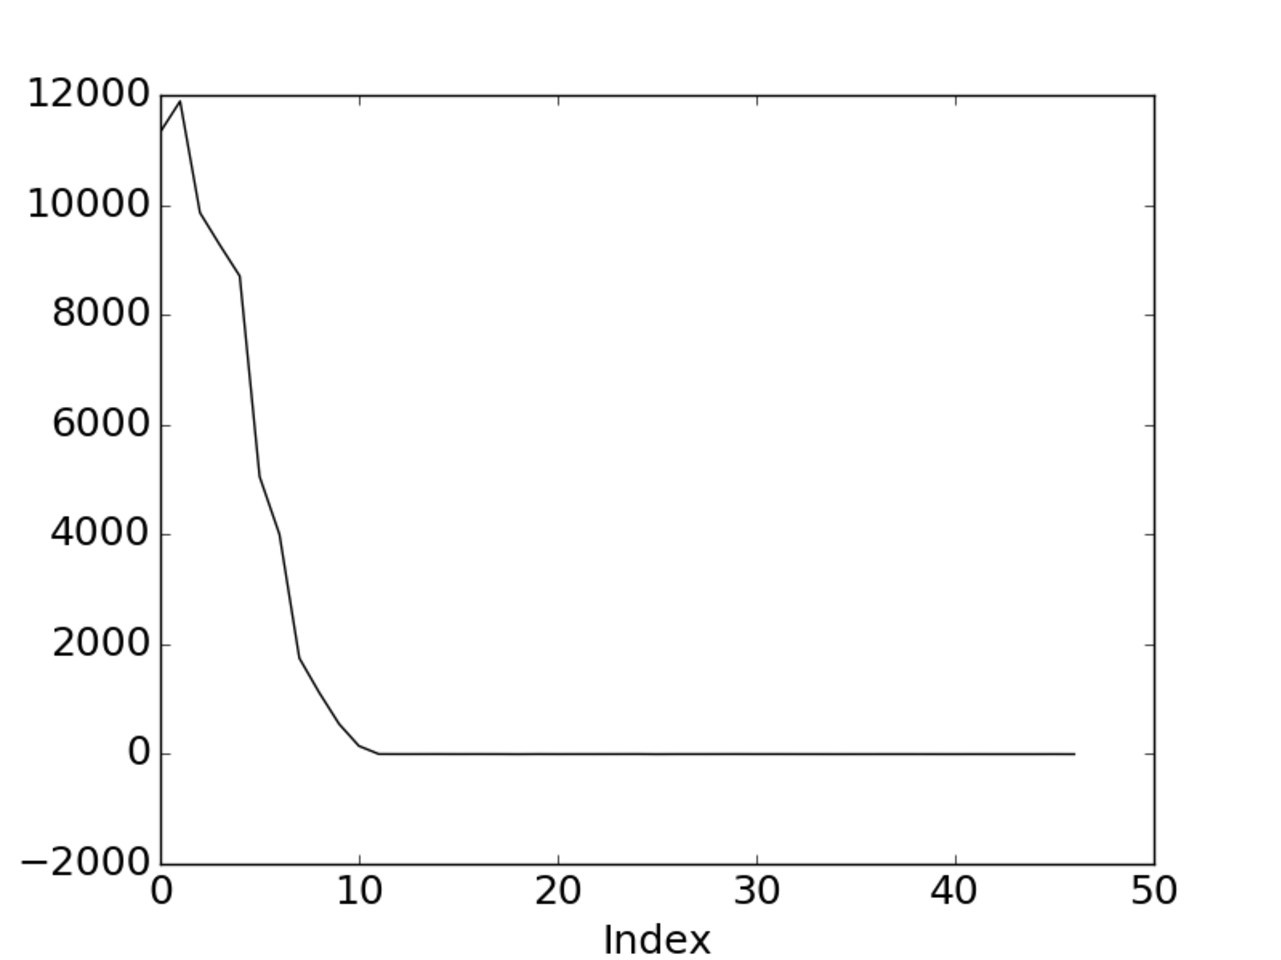
\includegraphics[width=\linewidth]{test_pics_6.pdf}
    \label{fig:examplestest6}
  \end{subfigure}
    \begin{subfigure}{.24\textwidth}
    \centering
        \caption{Weighted Kernel}   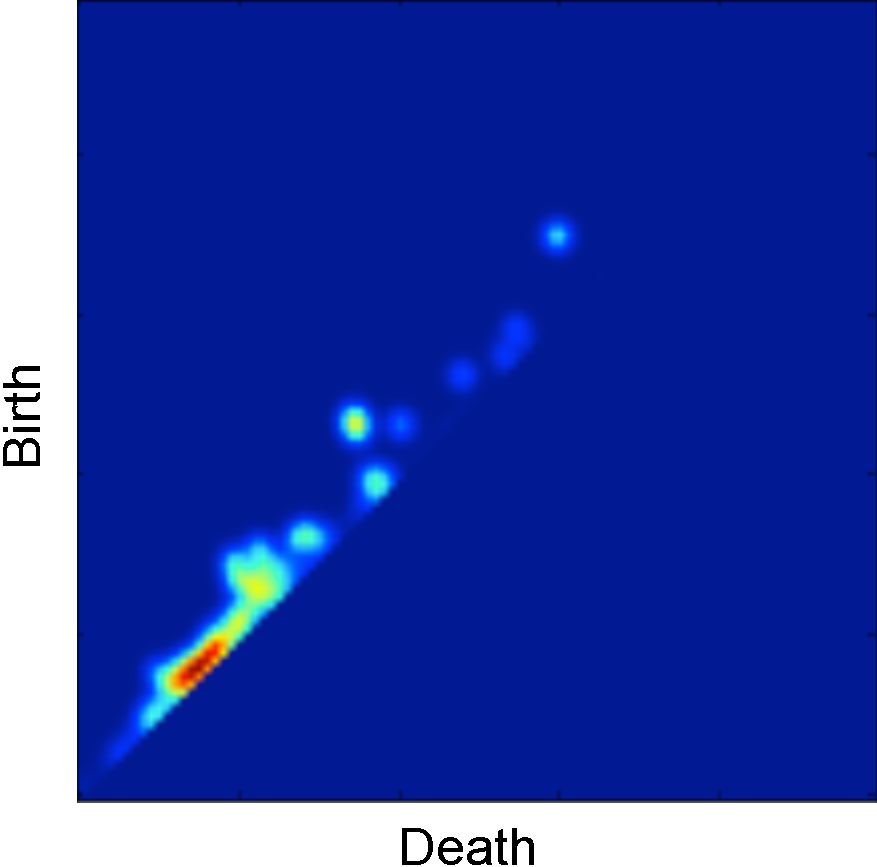
\includegraphics[width=\linewidth]{test_pics_7.pdf}
    \label{fig:examplestest7}
  \end{subfigure}
    \begin{subfigure}{.24\textwidth}
    \centering
        \caption{Persistent Image}  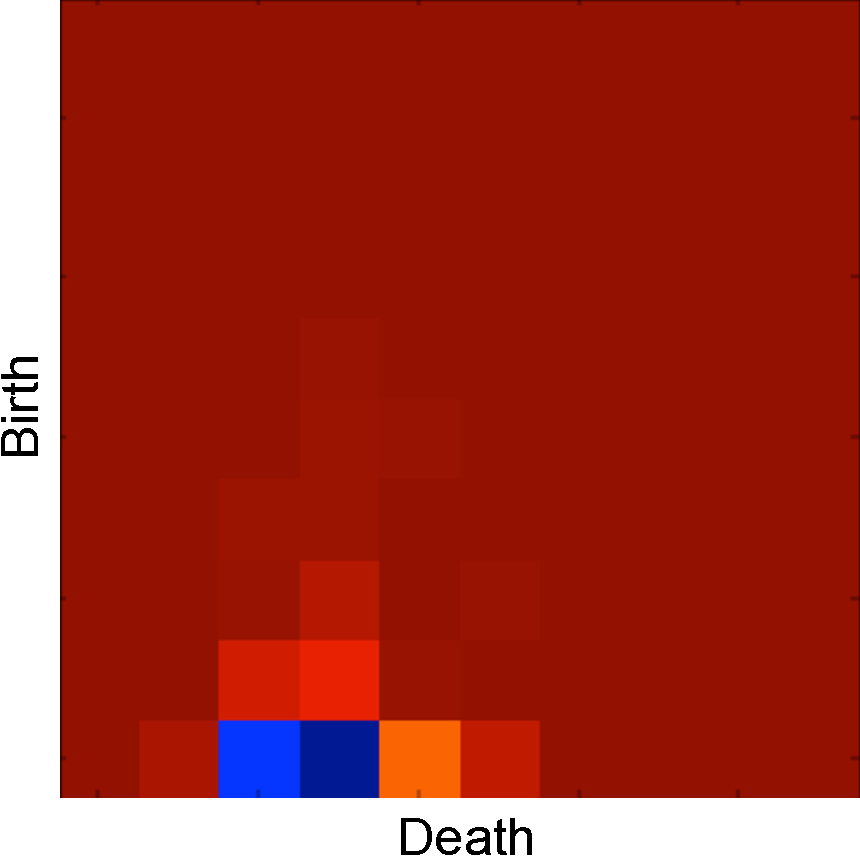
\includegraphics[width=\linewidth]{test_pics_8.pdf}
    \label{fig:examplestest8}
  \end{subfigure}
   \caption{Examples of test statistics used in the hypothesis tests. Figure \ref{fig:examplestest1} shows the point cloud used to generate figures \ref{fig:examplestest2} to \ref{fig:examplestest8}.}
   \label{fig:examples}
\end{figure}

% \begin{center}
% \begin{figure}[htp!]
%   \centering
%   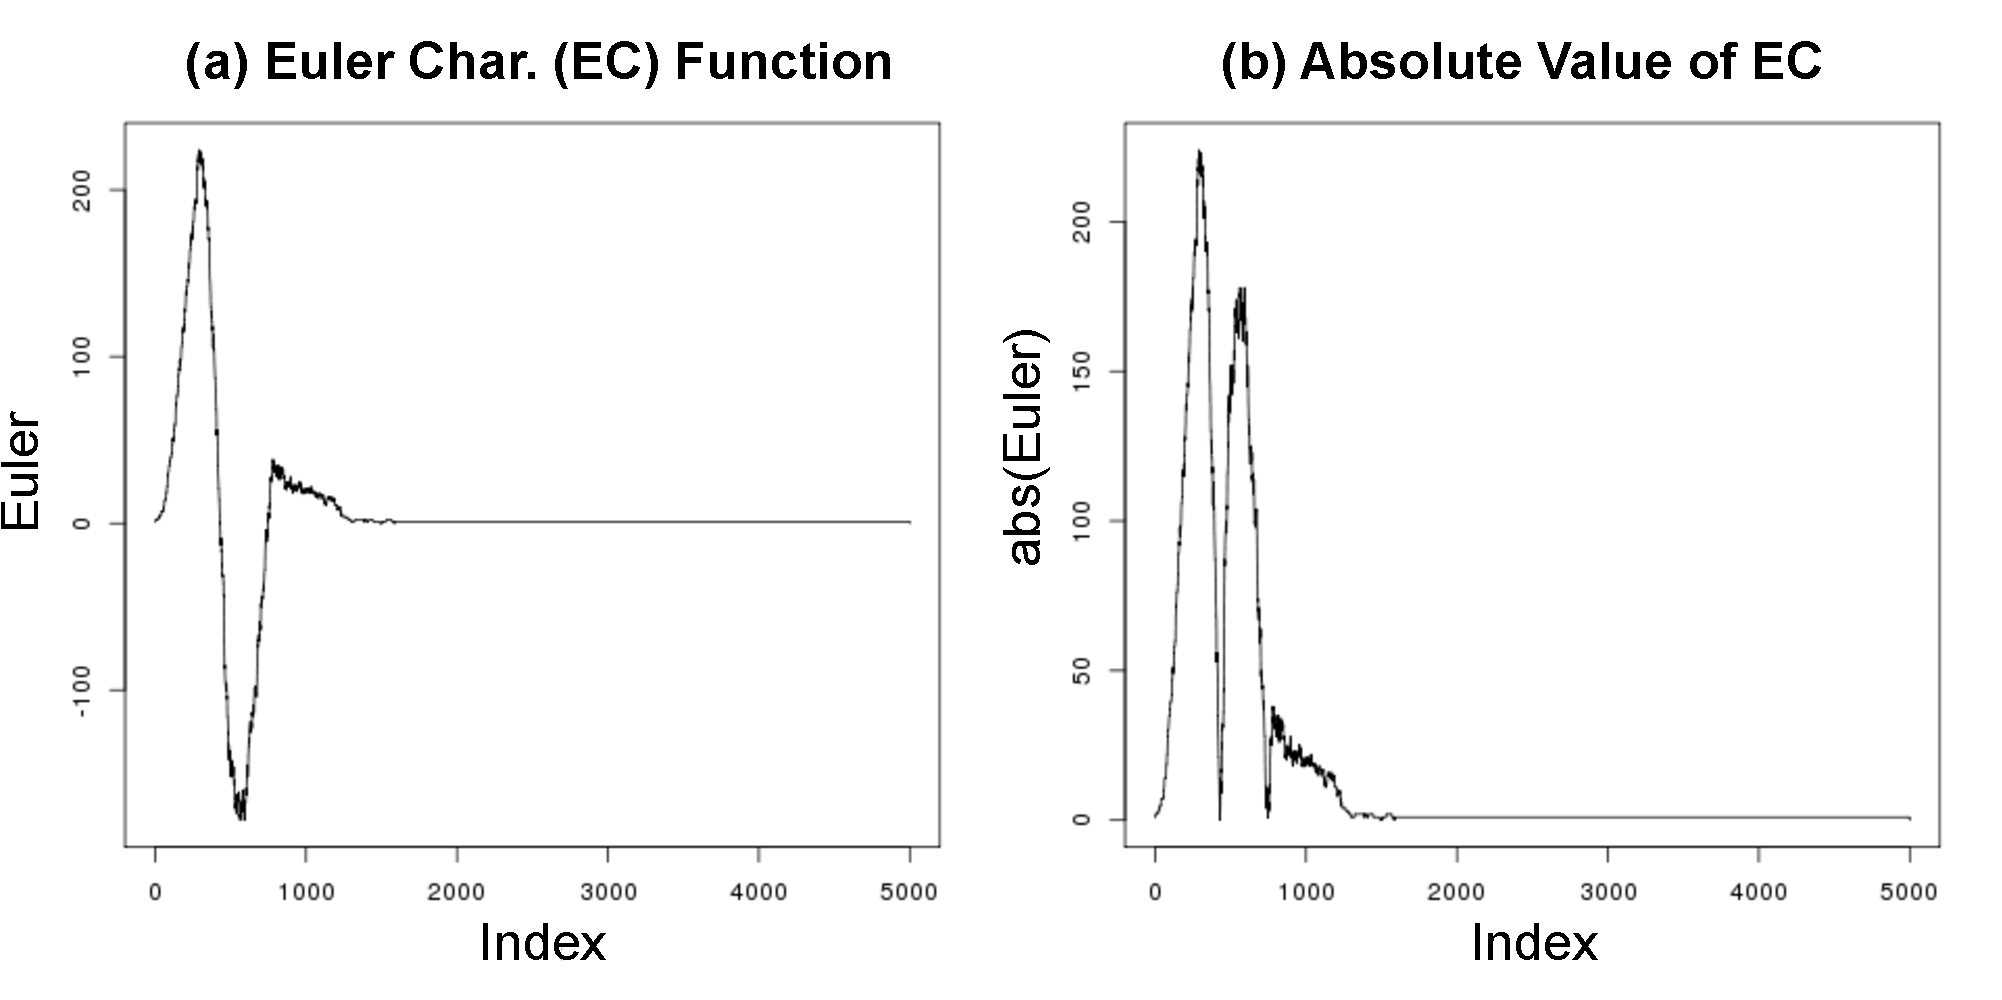
\includegraphics[width=0.7\linewidth]{example_euler.pdf}
%     \caption{(a) An Euler characteristic function created by plotting the Euler characteristic of a Voronoi foam model at each point beginning at time 0 until the last birth time. (b) The absolute value of the characteristic function that is integrated to produce the test statistic $E_{t}$.}
%     \label{fig:eulerexample}
% \end{figure}
% \end{center}

\paragraph{Silhouette Test (Sil)}
As with the Euler Characteristic (EC) function, a weighted silhouette summarizes a persistence diagram through a continuous function. Given a set of persistence diagrams (each with $N$ homology groups), each diagram is summarized by $N$ weighted silhouettes, and $N$ statistics, $\widehat{Sil}$, are calculated using the areas under the respective weighted silhouette, resulting in $N$ sets of statistics. In this manner,  each dimensional homology of a persistence diagram has its own test statistic, $\widehat{Sil}_{h}$, where $h$ represents a single homology group. This is preferred since the silhouette molded from connected components may be very different from the silhouette created from loops. We consider T-tests on each dimension ($\widehat{Sil}_0$, $\widehat{Sil}_1$, $\widehat{Sil}_2$), along with considering all dimensions in parallel ($\widehat{Sil}_{0:2}$) using a Hotelling $T^2$ test. 

\paragraph{Silhouette-Euler Characteristic (SilEC).}
Another method for considering all the individual silhouettes, $S_{i}(t)$, across dimensions $i = 0$, 1, and 2, simultaneously is a modified Euler characteristic function. Instead of calculating the alternating sum of Betti numbers, the Silhouette-Euler characteristic function (SilEC) is defined as the alternating sum of the individual silhouette functions across the threshold parameter, $t$. The statistic returned $\widehat{SilEC}$ is the integral of the absolute value of the summed function,  

\[ \widehat{SilEC} = \int_{t_{\min}}^{t_{\max}} | S_{1}(t) - S_{2}(t) + S_{3}(t) | \ \textup{d}t \]
As with EC test, a p-value is derived using a T-test.

\paragraph{Permutation Method.} Although not one of the nine approaches, the permutation method is frequently used in our nine tests and provides a very generic approach for calculating a p-value from any arbitrary test statistic. Assuming we observe two independent samples $X_{1}, \cdots, X_{n} \sim P$ and $Y_{1}, \cdots, Y_{n} \sim Q$, the two sample test problem is to test the hypothesis $H_{0} : P = Q$ versus the alternative $H_{1} : P \neq Q$. Assuming there is some arbitrary method of calculating a test statistic $T$ as a function of the data, we reject $H_{0}$ if $T > t$ where $t$ is a critical value. We choose $t$ such that if $H_{0}$ is true then $W(T > t) \leq \alpha$ where $W$ is the distribution of $T$ when $H_{0}$ is true. Permutation testing attempts to help us choose $t$ and find $W$ of $T$ under $H_{0}$. 

In the permutation method, the data is concatenated as a vector in the order \[X_{1}, X_{2}, \cdots, X_{n}, Y_{1}, Y_{2}, \cdots, Y_{n}\] and presented initial labels of $0$ or $1$ where all $X_{i}$ receive label 0 and all $Y_{i}$ receive label 1. If $H_{0}$ is true, then the entire data vector is an i.i.d sample from $P$ and the group labels are arbitrary. To test this, the group labels are randomly permuted and the test statistic is recalculated. This changes the values of $T$ but (under $H_{0}$), it should not change the distribution of $T$. The labels are permuted $N$ times and the p-value is

\[ p = \frac{1}{N}\sum^{n}_{j=1} I(T_{j} \geq T) \]

where $I$ is the indicator function. Therefore, the p-value is the fraction of times $T_{j}$ is larger than $T$. As $N$ approaches $\inf$, $p$ approaches the exact value.

\paragraph{Kernel Contour Test (KC).}
Rather than working with the raw persistence diagrams, the Kernel Contour Test (KC) uses a test statistic derived from a kernel two-sample test on the smoothed persistence diagram called the \emph{intensity function} \cite{chen2015statistical}.  The kernel two-sample test was first introduced for analyzing and comparing distributions with a maximum mean discrepancy (MMD) statistic \cite{gretton2012kernel}. The KC statistic used in this paper is computed for two sets of persistence diagrams and a hypothesis test is carried out using a permutation test.  The discrepancy between persistence diagrams is calculated as the integrated squared difference between two intensity functions instead of points directly from the persistence diagrams. The two-sample test statistic, $\widehat{KC}$, is defined as
\begin{sloppypar}
\begin{equation*}
\widehat{KC} = \frac{1}{n^{2}}\sum_{i=1}^{n}\sum_{j=1}^{n} K_{h}(X_{i}, X_{j}) - \frac{2}{mn}\sum_{i=1}^{n}\sum_{j=1}^{m}K_{h}(X_{i}, Y_{j}) + \frac{1}{m^{2}}\sum_{i=1}^{n}\sum_{j=1}^{n} K_{h}(Y_{i}, Y_{j}),
\end{equation*}
where $n$ and $m$ are the sizes of the two samples, and $\{X_1, \ldots, X_n\}$ and $\{Y_1, \ldots, Y_m\}$ are the two sets of intensity functions.  $K_{h}(X,Y)$ can be thought of as a similarity measure between intensity functions $X$ and $Y$, and in this case is a Gaussian kernel $K_{h}(X,Y) = exp(-\frac{||X - Y||^{2}}{h^{2}})$ with  $||X - Y|| = \int \left(X(t_1, t_2) - Y(t_1, t_2)\right)^2dt_1dt_2$  where $X(t_1, t_2)$ and $Y(t_1, t_2)$ are two intensity functions. The $h$ is a hyperparameter that sets the standard deviation of the Gaussian distribution used in the kernel $K_{h}$: a larger $h$ will reduce sensitivity to small differences between $X$ and $Y$, while a smaller $h$ will heighten sensitivity. The optimal $h$ value was found to be $0.1 \pm 0.04$ using greedy search from 0 to 5. A permutation test is used to calculate a p-value from the statistic.
% with $N$ permutations, and the p-value represents the fraction of times $T_{j}$ is larger than the observed $\widehat{GC}$ for any $j$,
\end{sloppypar}
% \[ \text{p-value} = \frac{1}{N} \sum_{j=1}^{N} I(T_{j} \geq T). \]

\paragraph{Weighted Kernel Test (WKC)}
Two disadvantages of the Kernel Contour Test (KC) shown above are (1) the tendency of the test to heavily weight dense clusters near the diagonal rather than sparse persistent features with longer lifespans, and (2) the possibility of the smoothed intensity function to ``spill over'' the diagonal as a product of the Gaussian kernel. The Weighted Kernel Test \cite{chen2015statistical} addresses both concerns with an adjusted kernel function. 

Let $b$ and $d$ denote the birth and death of a persistent feature, such that $\mathcal{D} = {(b_{j} , d_{j}) : j = 1, \cdots ,K}$ represents a persistence diagram where $K$ is the cardinality of persistent features. Given $\mathcal{D}$, we can estimate its intensity, $\kappa_{\tau}$ by

\[ \hat{\kappa}_{tau}(x,y) = \sum_{j}(d_{j} - b_{j})\frac{1}{\tau^{2}}K(\frac{x-b_{j}}{\tau})K(\frac{y-d_{j}}{\tau})\]

such that the sum is over all persistent features, $K$ is a symmetric kernel function (such as 1D Gaussian where the mean and standard deviation are estimated by the sample), and $\tau$ is a smoothing parameter. This statistic is calculated over a two-dimensional grid 
\[ \{ (x, y) \textup{ s.t. } b_{min} \leq x \leq b_{max} \wedge d_{min} \leq y \leq d_{max} \} \]

where $b_{min} = \textup{min}(\{b_{j}\}^{K}_{j=1})$, $d_{min} = \textup{min}(\{d_{j}\}^{K}_{j=1})$, $b_{max} = \textup{max}(\{b_{j}\}^{K}_{j=1})$, and $d_{max} = \textup{max}(\{d_{j}\}^{K}_{j=1})$. A step size $h_{x}$ between adjacent pairs $(x_{i}, y_{j})$, $(x_{i+1}, y_{j})$, and $h_{y}$ between pairs $(x_{i}, y_{j})$, $(x_{i}, y_{j+1})$ control the size of the grid ($h_{x} = h_{y} = 0.01$ used in practice). This Weighted Kernel Contour statistic \cite{chen2015statistical} uses the difference between the birth and death of each persistent feature as the weight for that feature. Therefore, features near the diagonal will have very little effect, reducing spill over, and sparse features with long lifespans (generally more interesting topologically) will contribute more. 

To calculate the p-value, the grid $\{x, y\}$ is flattened into a vector where each index represents an abstracted topological feature, and as with the KC test, an asymptotic argument (permutation test) is used. The WKC test is performed independently for each homology, resulting in three tests: WKC(0), WKC(1), and WKC(2).

\paragraph{Persistent Image Test (PI)} The Persistent Image test \cite{adams2015persistent} is a variation of the WKC test with an alternative kernel function and sub-sampling. Let $\mathcal{D} = {(b_{j} , d_{j}) : j = 1, \cdots ,K}$ be a persistence diagram where $K$ is the number of persistent features. Unlike WKC, the PI test first transposes the persistent diagram using the linear transformation $T: \mathbb{R}^{2} \rightarrow \mathbb{R}^{2}$ where $T(x,y) = (x, y-x)$. Therefore, let $T(\mathcal{D})$ represent the transformed diagram with the new birth-persistence coordinates. Let $K_{u} : \mathbb{R}^{2} \rightarrow \mathbb{R}$ be a differentiable probability distribution with mean $u = (u_{x}, u_{y})$. In our applications, we choose this distribution to be the normalized symmetric 2D Gaussian with mean $u$ and variance $\sigma^{2}$. 

\[ K_{u}(x,y) = \frac{1}{2\pi\sigma^{2}}e^{-[(x - u_{x})^{2} + (y-u_{y})^{2}]/2\sigma^{2}} \]

Finally, let $f : \mathbb{R}^{2} \rightarrow \mathbb{R}$ be a non-negative weighting function that is zero along the horizontal axis, continuous and differentiable. $f$ is chosen to only depend on the rotated vertical persistence coordinate $y$, and like WKC, weight points of higher persistence (lifespan) more heavily. In our applications, we use a piecewise linear weighting function that was found to be stable. Given $b > 0$, define $f_{b}$ as

\[ f_{b}(t) = \rightarrow \left\{\begin{matrix}
0 & \textup{if } t \leq 0 \\ 
\frac{t}{b} & \textup{if } 0 < t < b\textup{, and}\\ 
1 & \textup{if } t \geq b 
\end{matrix}\right. \]

Given $f$, $K$, and $T(\mathcal{D})$, we can define a persistence surface \cite{adams2015persistent}, $\rho_{\mathcal{D}} : \mathbb{R}^{2} \rightarrow \mathbb{R}$ as 

\[ \rho_{\mathcal{D}}(x, y) = \sum_{u \in T(\mathcal{D})} f(u)K_{u}(x,y) \]

Like the WKC test, $\rho$ is calculated over the two-dimensional grid \[ \{ (x, y) \textup{ s.t. } b_{min} \leq x \leq b_{max} \wedge d_{min} \leq y \leq d_{max} \} \]. In our applications, the step sizes $h_{x}$ and $h_{y}$ were chosen to make the grid size 30 by 30. Given $\rho_{\mathcal{D}}$, a persistence image \cite{adams2015persistent} $I(\rho_{\mathcal{D}})_{p}$ is defined as a grid of pixels calculated from convolving the persistent surface with a uniform matrix of size $n$ by $n$ of 1's. In order words, $I(\rho_{\mathcal{D}})_{p} = \int\int_{p} \rho_{\mathcal{D}} \textup{ d}y\textup{d}x$. This matrix is then flattened into a 1D vector.  The p-value accuracy of the PI framework is found to be robust to the choice of the convolution filter size. In our applications, a filter size of 3 is used, resulting in a 10 by 10 matrix, or 100 length vector when flattened.

Unlike the WKC test, the PI test combines all homologies into a single statistic \cite{adams2015persistent}. Suppose the homologies $H_{0}, \cdots, H_{k}$ are computed. One can concatenate the PI vectors for $H_{0}, \cdots, H_{k}$ into a single vector representing all dimensions simultaneously. Like the WKC test, the p-value is calculated using the permutation method, but only once for all 3 homologies.

\paragraph{Two-point Correlation Function Test (CORR)}
{\color{red}  Jessi:  revise section, explain why to consider this}
The Two Point Correlation Test \cite{landy1993bias}, unlike previous methods, quantitatively measures large scale structure through tracing the amplitude of clustering as a function of scale. Such a trace is determined by the correlation function, $\xi(r)$. $\xi(r)$ is defined as the measure of the excess probability d$P$, above the expectation for an unclustered random Poisson distribution of finding a cluster in a given volume element d$V$ at a separation radius $r$ from another cluster such that 
\[ \textup{d}P = n[1 + \xi(r)] \textup{ d}V \] where $n$ is the mean number density of the sample dataset.

$\xi(r)$ is measured by counting pairs of clusters as a function of the separation radius compared to the count for an unclustered distribution. To do this, one must construct a \textit{random catalog} that has similar three dimensional coverage as the data but is populated with randomly distributed points. Define $DD$, $DR$, $RR$ as counts of pairs of clusters (in bins of varying separation radii) in the data, between the data and the random catalog, and in the random catalog, respectively; let $n_{D}$, $n_{R}$ respectively define the mean number of densities of clusters in the data and random catalogs. The correlation function is estimated by \cite{landy1993bias}:

\[ \xi = \frac{1}{RR}\left[DD\left(\frac{n_{R}}{n_{D}}\right)^{2} - 2DR\left(\frac{n_{R}}{n_{D}}\right) + RR\right] \]

Provided a point cloud, clusters are derived and compared to a random catalog that is generated within the same dimensional space. Unlike other statistics, because $\widehat{CORR}$ is not dependent on persistence diagrams, only a parallel test is applicable in which clustering occurs along all three dimensions. A correlation function, $\xi$ can then be calculated. The test statistic, $\widehat{CORR}$ is defined by the area under the absolute value of $\xi$.

\[ \widehat{CORR} = \int_{r} \left | \xi(r) \right | \textup{ d}r \]

To generate the random catalog $\left | \mathcal P \right |$ points were drawn from a Uniform distribution $\textup{U}(0, max(\mathcal P))$. If $\mathcal P$ was standardized, points were sampled from $\textup{U}(0, 1)$. 

%%%%%%%%%%%%%%%%%%%%%%%%%%%%%%%%%%%%%%%%%%%%%%%%%%%%%%%
%% SECTION: SIMULATION STUDY
%%%%%%%%%%%%%%%%%%%%%%%%%%%%%%%%%%%%%%%%%%%%%%%%%%%%%%%

\section{Simulation Study}
\label{sec:simulation}

To evaluate the performance of the proposed test statistics for the two-sample hypothesis tests, we carried out a simulation study by generating realizations of web-like spatial structures.  The simulation model is discussed in detail below.  After discussing the simulation model and simulation test results, we explain a way to deal with possible scaling differences in the two samples; ultimately the rescaling is done on the persistence persistence diagram.

\subsection{Simulation model} \label{sec:sim_model} %--------------------------------------
Motivated by LSS, we developed our simulation model to approximate the Cosmic Web, though these structures appear in other areas of science as well.  In particular, we drew from ideas that use Voronoi tesselations to model the filament structure of the Universe, known as \emph{Voronoi Foam} \cite{icke1987fragmenting, icke1991galaxy, van2007voronoi}.  The Voronoi Foam model offers an approximation to the distribution of matter in the Universe at large scales (e.g. galactic clusters, filaments, walls), but not scales (e.g. small groups of galaxies) \cite{icke1991galaxy}.

The cells of the Voronoi tesselation become the cosmological voids, the outline of the cells are the filaments and walls, and the points of intersection are the superclusters (large clusters of galaxies).  Once the tesselation is defined, points are added according to several parameters - the points can represent individual galaxies, clusters of galaxies, or dark matter halos (which would host gravitationally-bound galaxies or galactic clusters).
The elements of our approximate Voronoi Foam model include (i) the number of voids (the number of cells in the Voronoi tesselation), (ii) the number of galaxies/clusters/halos (the number of points to generate), and (iii) the percentage of the points that should fall on the cluster, filaments, and walls, see Table~\ref{table:voronoisettings}.   
In this simulation study, we varied the filament percentage (percFil) from 0.1 to 0.9 by a 0.1 step size.  

\begin{table}[htp!]
\begin{center}
\begin{tabular}{ l|l|l } 
Abbrev & Definition & Value \\ 
\hline
percWall & Percentage of particles on the walls & $0.98 - p_{f}$ \\ 
percFil & Percentage of particles on the filaments & $p_{f}$ \\ 
percClust & Percentage of particles in the clusters & 0.02 \\ 
\end{tabular}
\end{center}
\caption{Parameters of LSS model. For the simulation study, $p_{f}$ will vary from 0.1 to 0.9.}
\label{table:voronoisettings}
\end{table}


Figure~\ref{fig:vf} displays the construction procedure of one realization of our simulation model:  (i) First a grid is defined at a specified resolution within a specified volume; (ii) then a specified number of points are randomly selected within the volume - these will be used to define the Voronoi tesselation and will act as voids (these will be called \emph{void points}; (iii) the nearest void point to each grid point is found and stored, call this the \emph{void label} of a grid point; (iv) the void labels of the eight nearest neighbors of each grid point is noted - if there are more than three unique void labels among the eight then that grid point is assigned to be a cluster point, if there are exactly three unique void labels among the eight nearest neighbors then that grid point is assigned to be a filament point, and if there are exactly two unique void labels among the eight nearest neighbors then that grid point is assigned to be a wall point. The black, empty circles in Figures~\ref{subfig:cluster}, \ref{subfig:fil}, \ref{subfig:wall} display the grid points that were selected to be cluster points, filament points, and wall points, respectively.  Depending on the parameter assignments in Table~\ref{table:voronoisettings} and the total desired sample size of dataset, the number of points are randomly selected among the cluster, filament, and wall points.  Specified Gaussian noise is also added to the selected points so they do not fall exactly on the defined grid.


\begin{figure*}[t!]
    \centering
    \begin{subfigure}[t]{0.5\textwidth}
        \centering
        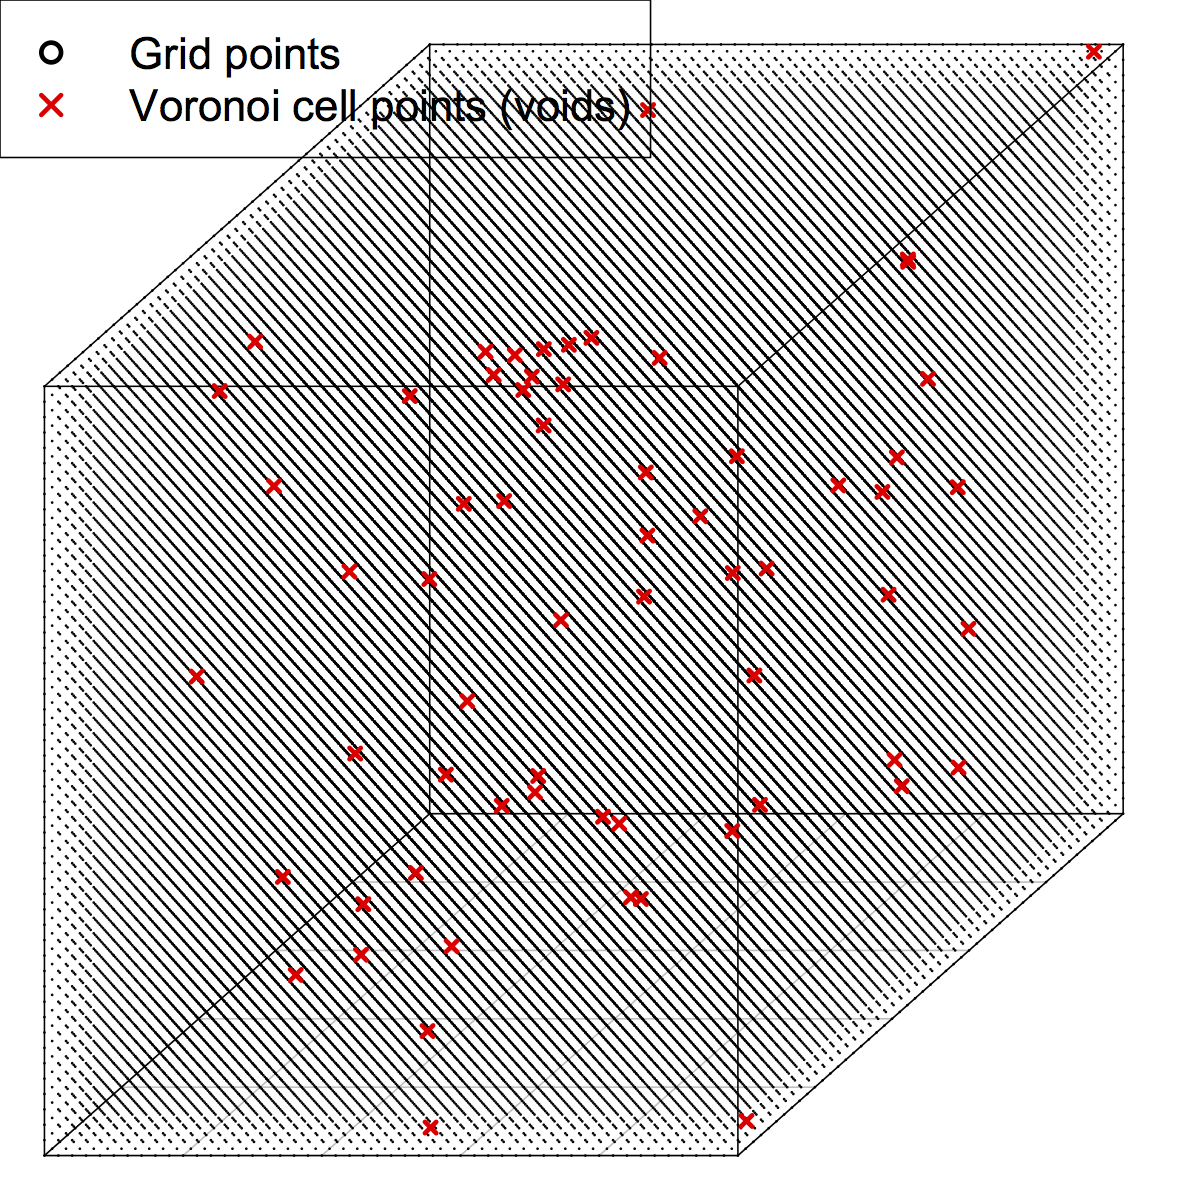
\includegraphics[height=2.25in]{vf_grid.png}
        \caption{Grid and selected voids} \label{subfig:grid}
    \end{subfigure}%
    ~ 
    \begin{subfigure}[t]{0.5\textwidth}
        \centering
        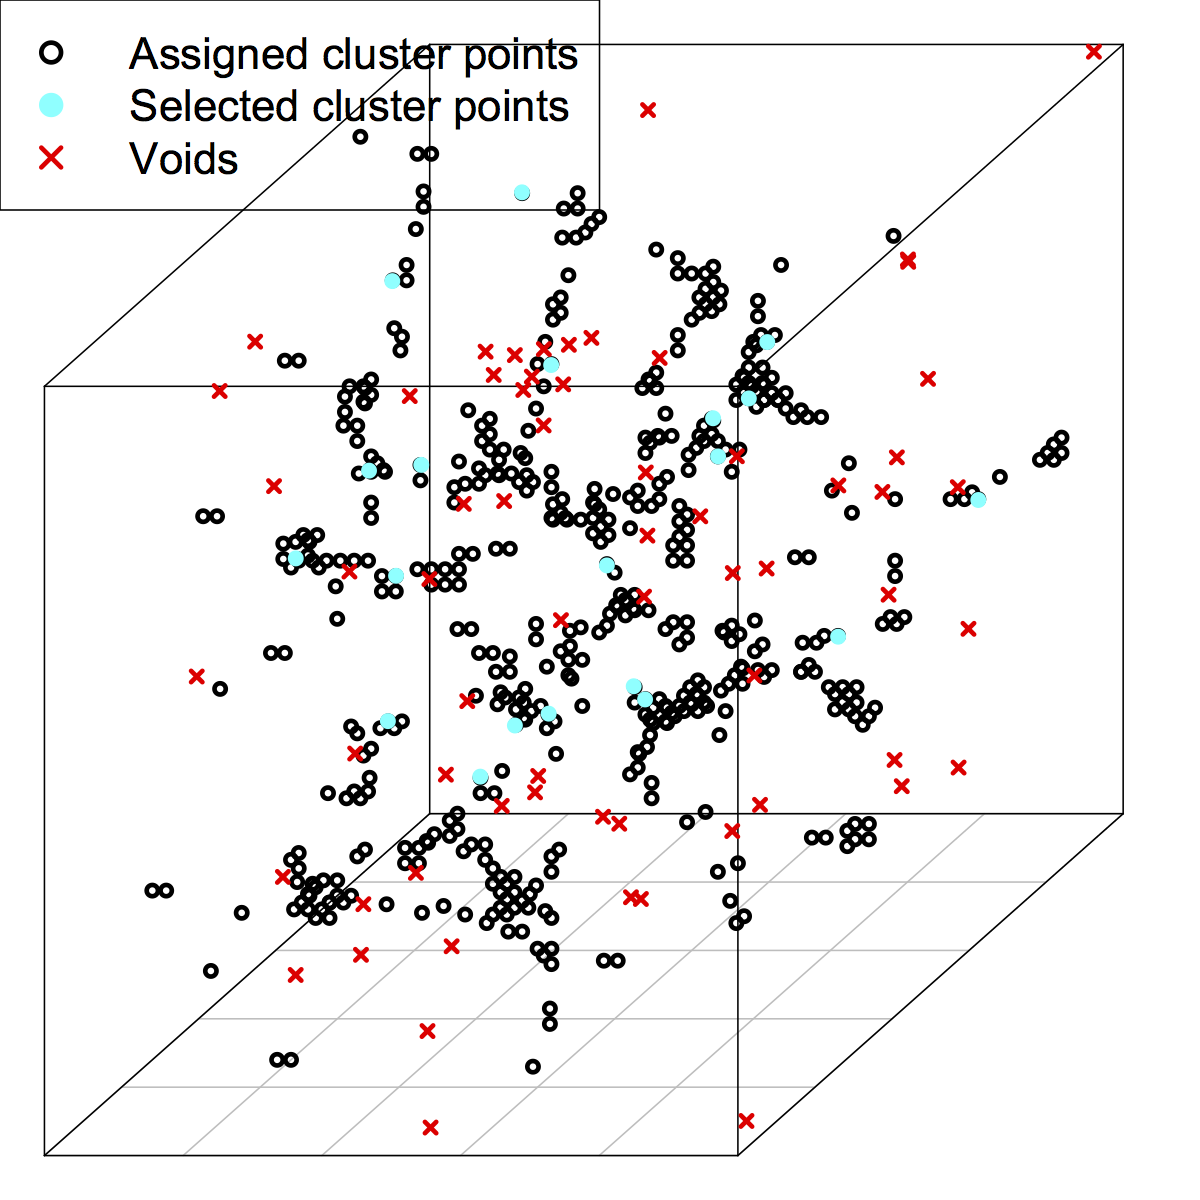
\includegraphics[height=2.25in]{vf_cluster.png}
        \caption{Cluster points} \label{subfig:cluster}
    \end{subfigure} \\
    
     \begin{subfigure}[t]{0.5\textwidth}
      \centering
    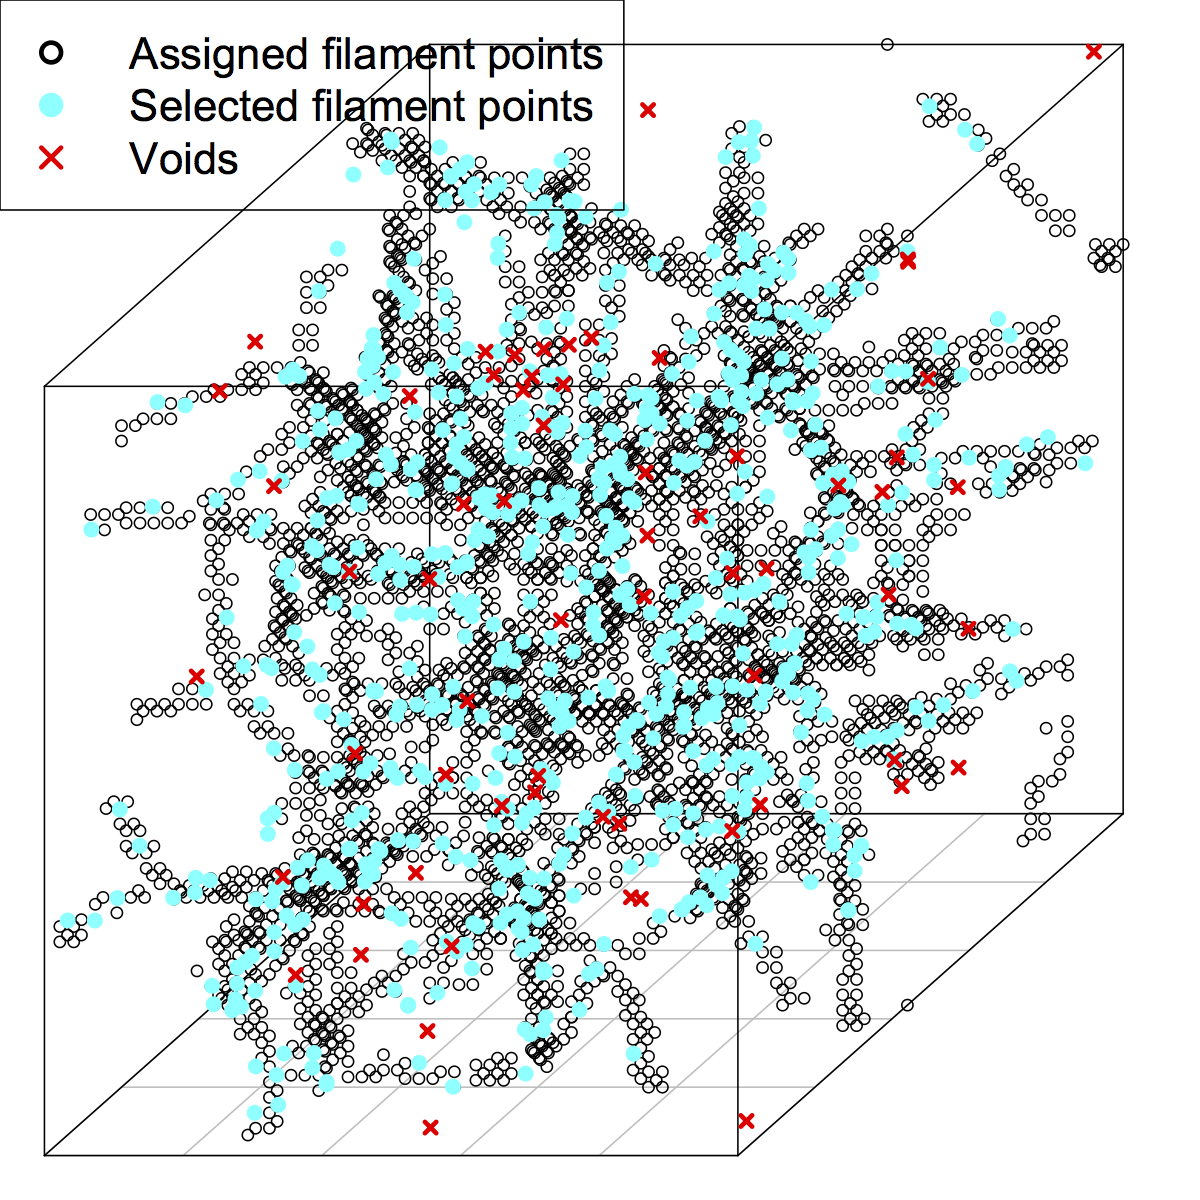
\includegraphics[height=2.25in]{vf_fil.png}
     \caption{Filament points} \label{subfig:fil}
    \end{subfigure}%
    ~ 
    \begin{subfigure}[t]{0.5\textwidth}
        \centering
        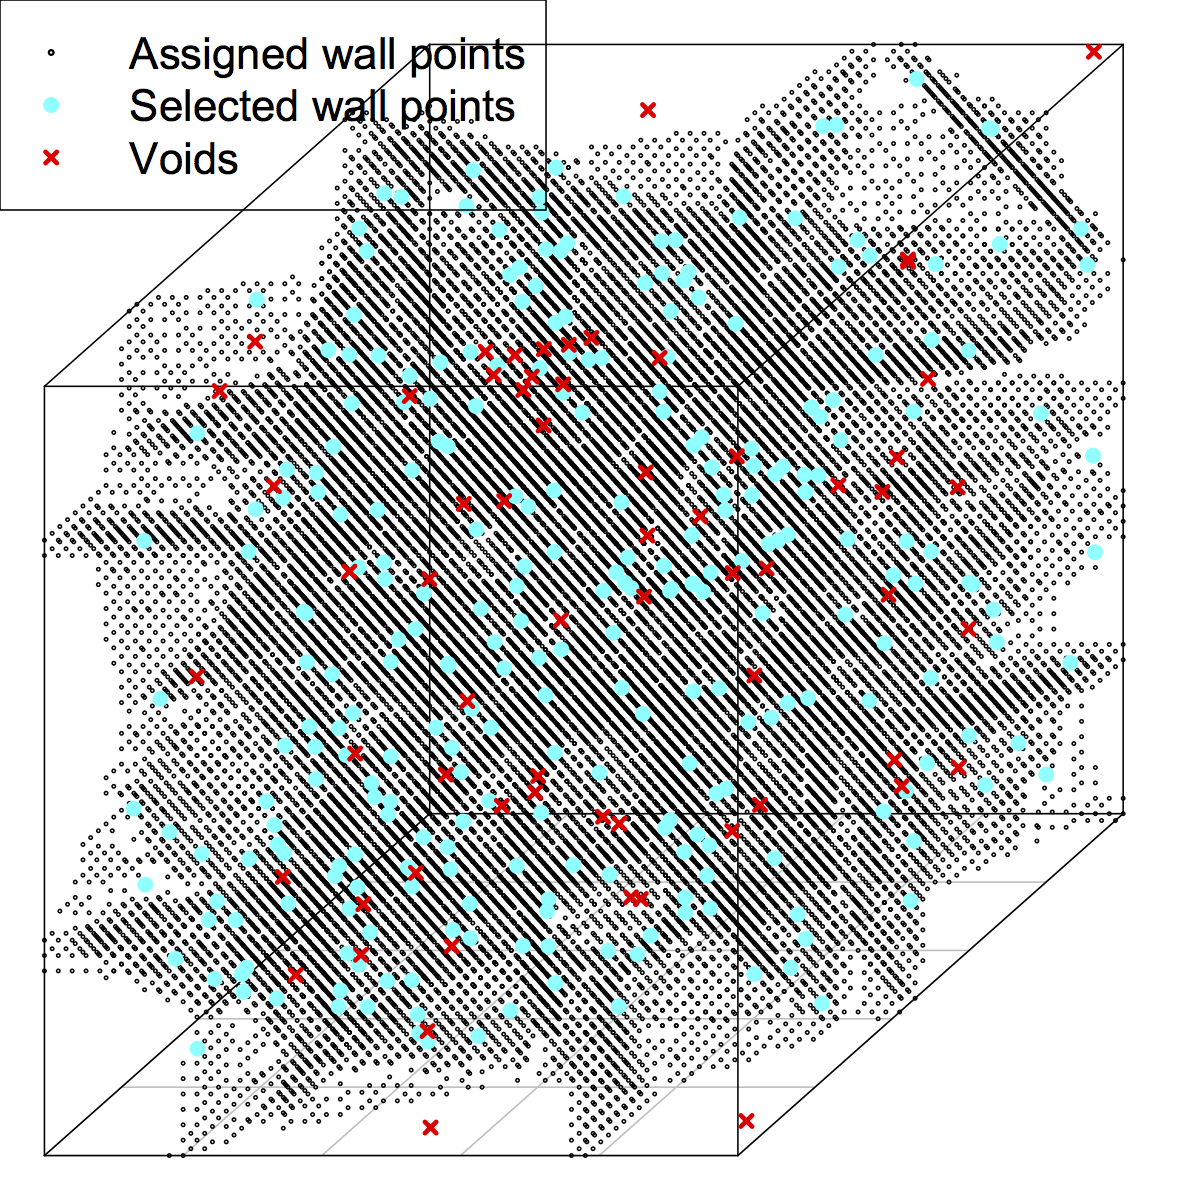
\includegraphics[height=2.25in]{vf_wall.png}
        \caption{Wall points} \label{subfig:wall}
    \end{subfigure}
    \caption{Simulation model construction.  (a) A grid is defined and points are randomly selected to define the Voronoi tesselation - the Voronoi cells are the voids.  (b) - (d) Based on the location of the voids and the grid, points are defined to be cluster points, filament points or wall points - these are the empty black circles.  Based on the values assigned from Table~\ref{table:voronoisettings}, a number of points are randomly selected from the assigned points to be in the dataset.} \label{fig:vf}
\end{figure*}

% introduced the Voronoi foam as a packing of polyhedral units with walls representing pancakes, edges representing filaments, and vertices representing clusters in the galaxy. Icke showed that the Voronoi foam is an appropriate model for a 10-500 Mpc scale Universe with pressure-free Newtonian gravitational collapse. Statistical study showed that the spatial two-point correlation of Voronoi foams has a power law behavior with close to identical amplitude and slope as that of actual Abell clusters \cite{vanvoronoi}. 
% A Voronoi foam model, is generated from a tessellation, where the edges of each cell represent filaments and the faces of the cell, enclosed voids. Given a plane with fixed size, such a tessellation partitions the plane into cellular regions with nuclei. Every cell territory is defined as the set of points equal or closer to that cell's nuclei than any other. To produce a simulation in polynomial time, each point in the plane is compared to the $k$ closest nuclei using a nearest neighbor algorithm where $k$ is chosen to be a small integer. Gaussian noise is added to perturb the plane and inject randomness. Because the nuclei number and the plane size are variable, the points in the simulation representing filaments, clusters, and walls are variable as well. By choosing a reasonable percentage of filaments and related structures, Voronoi simulations are to approximate the topology and LSS of true simulations of the observable Universe. By varying these percentages and repeating simulations, one can quickly generate a large, labeled data sets for hypothesis testing. Our interest primarily was gauging the effect of changing the percent filament in the Voronoi tessellation on the ability of the hypothesis tests to distinguish two foam models sampled from different tessellations. 


Examples of three separate Voronoi foam models of percFil 0.1, 0.5, 0.9 are displayed in Figure~\ref{fig:percfilexample} along with their corresponding persistence diagrams. One can see that the as the percFil (the percentage of points that are part of filaments) increases, the web-like structure becomes more pronounced.

\begin{center}
\begin{figure}[htp!]
  \centering
  \begin{subfigure}{.32\textwidth}
    \centering
    \caption{PercFil 0.1 (Voronoi)} 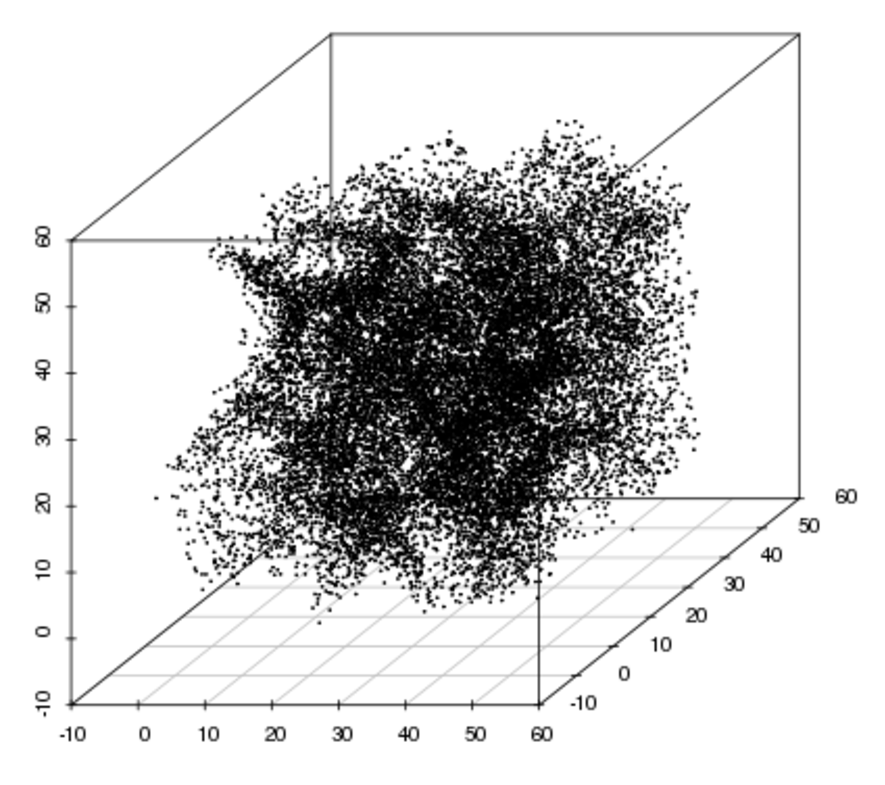
\includegraphics[width=0.6\linewidth]{percfil01voronoi.pdf}
    \label{fig:percfil01voronoi}
  \end{subfigure}
    \begin{subfigure}{.32\textwidth}
    \centering
    \caption{PercFil 0.5 (Voronoi)} 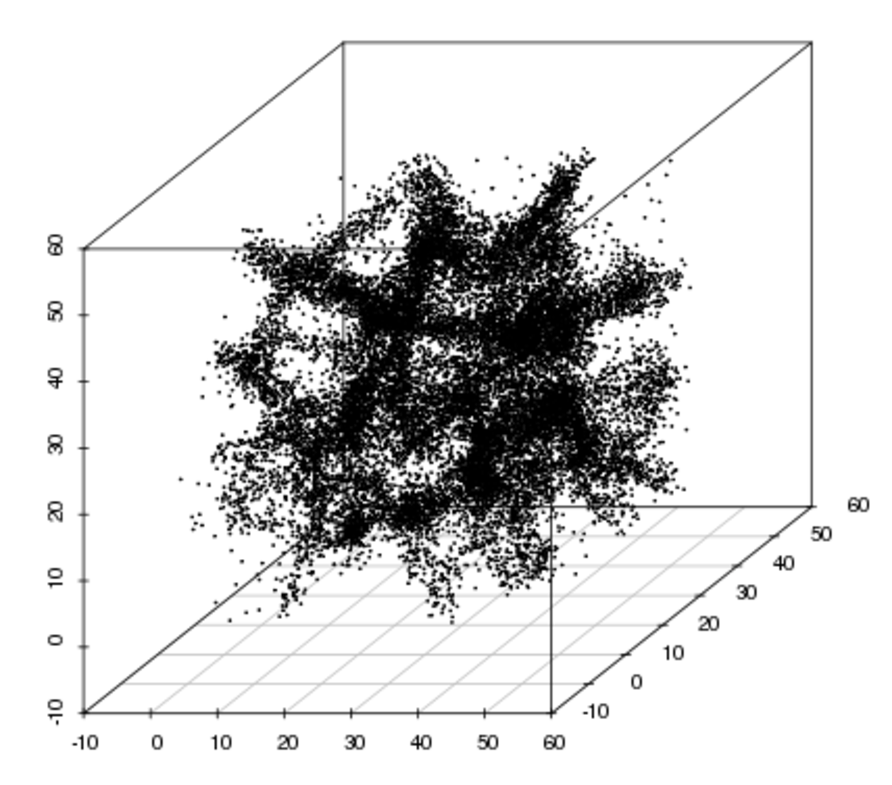
\includegraphics[width=0.6\linewidth]{percfil09voronoi.pdf}
    \label{fig:percfil09voronoi}
  \end{subfigure}
    \begin{subfigure}{.32\textwidth}
    \centering
    \caption{PercFil 0.9 (Voronoi)} 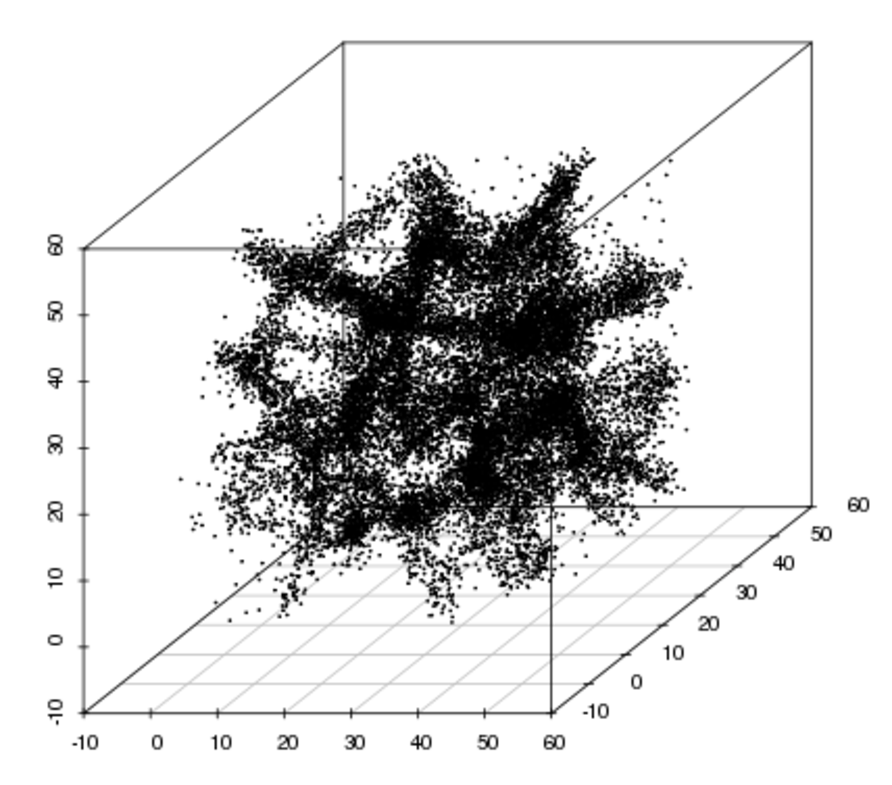
\includegraphics[width=0.6\linewidth]{percfil09voronoi.pdf}
    \label{fig:percfil09voronoi}
  \end{subfigure}
    \begin{subfigure}{.32\textwidth}
    \centering
    \caption{PercFil 0.1 (PD)}  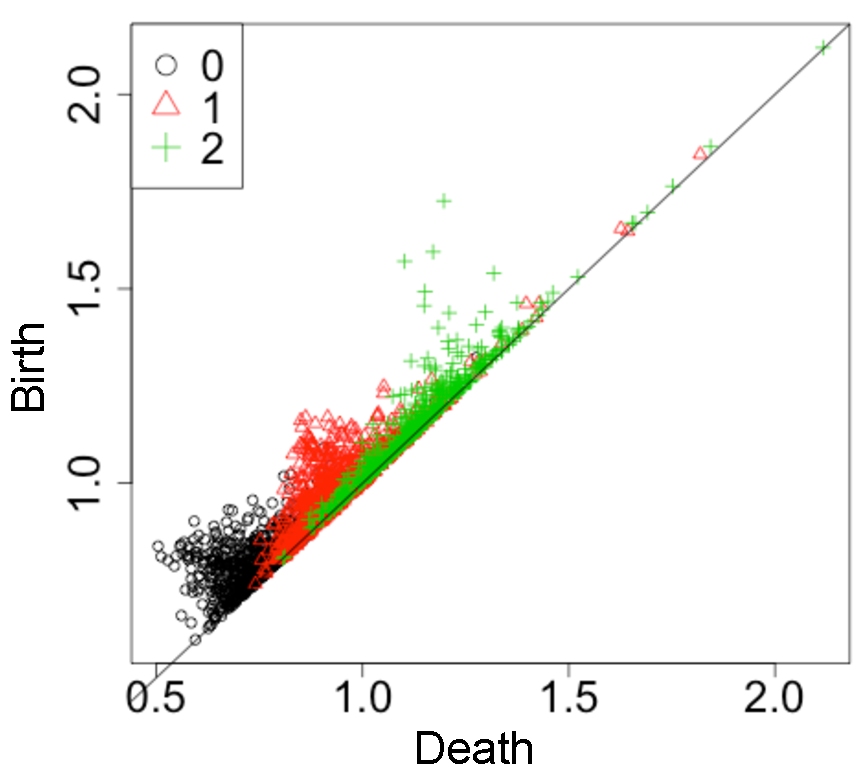
\includegraphics[width=0.6\linewidth]{percfil01pd.pdf}
    \label{fig:percfil01pd}
  \end{subfigure}
    \begin{subfigure}{.32\textwidth}
    \centering
    \caption{PercFil 0.5 (PD)}  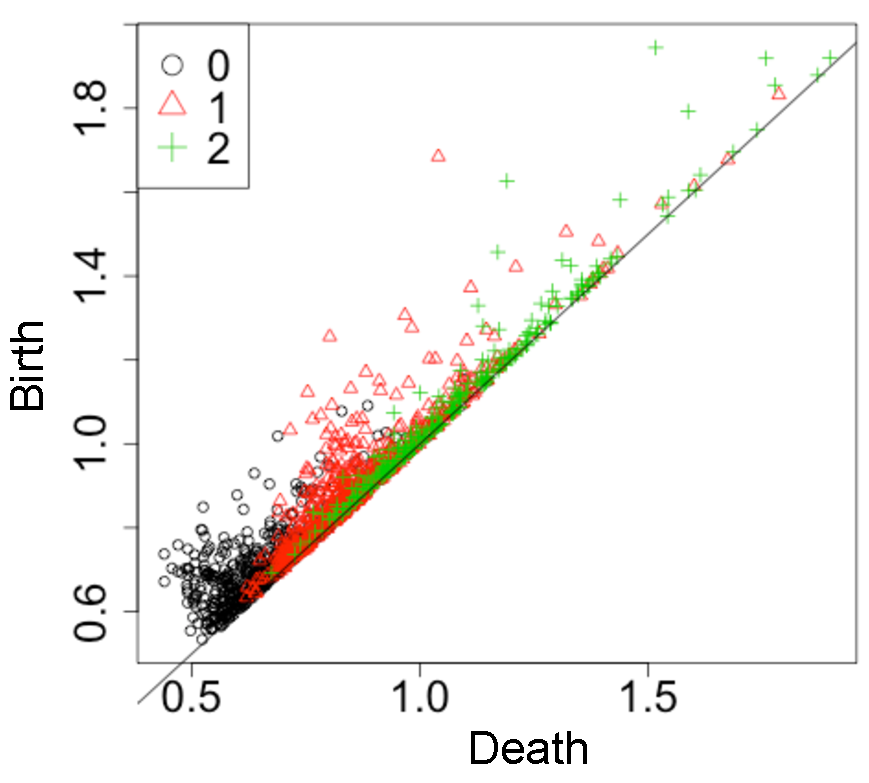
\includegraphics[width=0.6\linewidth]{percfil09pd.pdf}
    \label{fig:percfil09pd}
  \end{subfigure}
    \begin{subfigure}{.32\textwidth}
    \centering
    \caption{PercFil 0.9 (PD)}  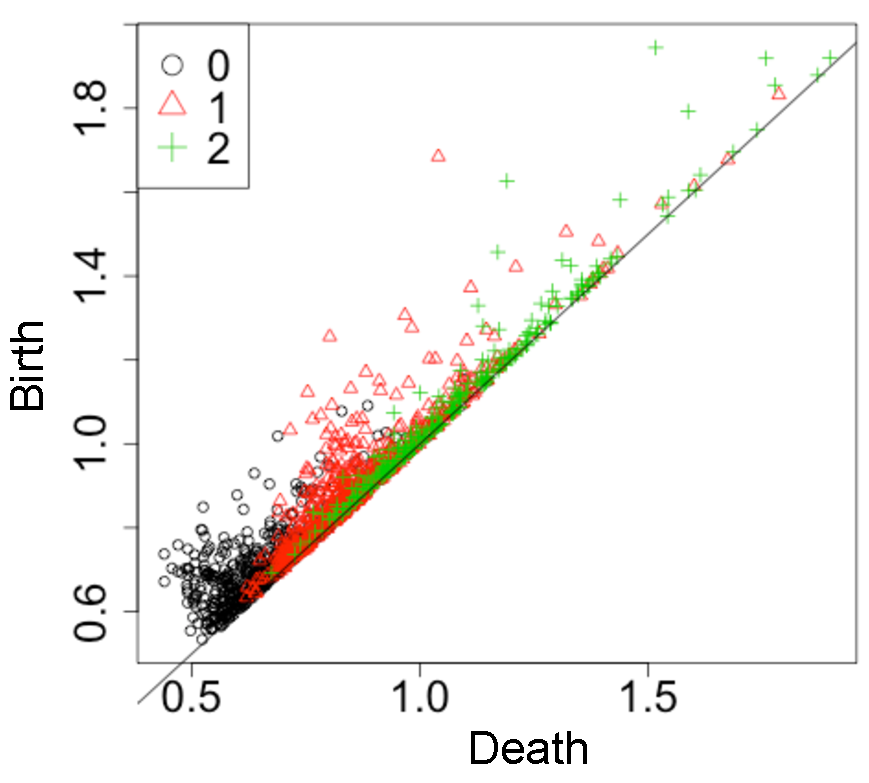
\includegraphics[width=0.6\linewidth]{percfil09pd.pdf}
    \label{fig:percfil09pd}
  \end{subfigure}
    \caption{(a) PercFil 0.1; (b) PercFil 0.5; (c) PercFil 0.9; (d-f) Corresponding persistence diagrams (PD) for point clouds (a-c). All other parameters are defined based on Table~\ref{table:voronoisettings}.}
    \label{fig:percfilexample}
\end{figure}
\end{center}







\subsection{Simulation study results} \label{sec:results1} %--------------------------------------
The simulation models used in this paper were generated under $1.25 \times  10^{5}$ box volume, $0.1$ resolution, $1 \times  10^{4}$ points, $64$ cells (voids), 0.02 percClust, and $[0.1, 0.9]$ percFil and $[0.08, 0.88]$ percWall. Persistent homology is calculated using distance-to-measure (DTM) with a $0.01$ tuning parameter. Persistence diagrams are preprocessed to remove the known 0-dimensional artifact wherein persistent homology algorithms produce a vestigial $H_{0}$ element with birth time of 0 and a death time of $\infty$ (with exception to the Euler characteristic function in which the artifact is preserved).  
The hypothesis tests were performed on 100 independent iterations of 15 independent realizations from each of the two populations.
The 15 independent datasets are each generated using a percFil setting from 0.1 to 0.9; we also include a control model with a percFil of 0.1.  (Hence 9 sets of 15 datasets, repeated 100 times.)
Using the proposed hypothesis tests, each of the variable models will be compared to the control (with percFil of 0.1). 
More specifically, given the data drawn from a model with percFil $p$, each of the proposed test statistics are used to compute a  p-value for the test $H_0: \mathcal 
P^{(1)} = \mathcal P^{(2)}$ vs. $H_1: \mathcal P^{(1)} \neq \mathcal P^{(2)}$, 
based on two samples of persistence diagrams, $\{\mathcal 
P_1^{(1)}, \ldots, \mathcal P_{15}^{(1)}\}$ drawn from the model with percFil = 0.1, and $\{\mathcal P_1^{(2)}, \ldots, 
\mathcal P_{15}^{(2)}\}$ drawn from the model with percFil = $p$, $p = 0.1, 0.2, \ldots, 0.9$.  
(Recall that $\mathcal P^{(1)}$ and $\mathcal P^{(2)}$ are the true underlying 
distributions of persistence diagrams for group 1 and 2, respectively.)  
Similar tests were also completed against a control model with 0.9 percFil, and similar results were found. The simulation study results are displayed in Figure~\ref{fig:linesUnnorm}, which displays the median p-values from the proposed test statistics: (i) Euler-based tests, (ii) Silouette-based tests, (iii) Kernel-based  tests, (iv) Weighted Kernel-based tests, (v) Correlation-based tests and (vi) a comparison of the best results from each category.

\begin{figure}[htp!]
  \centering
  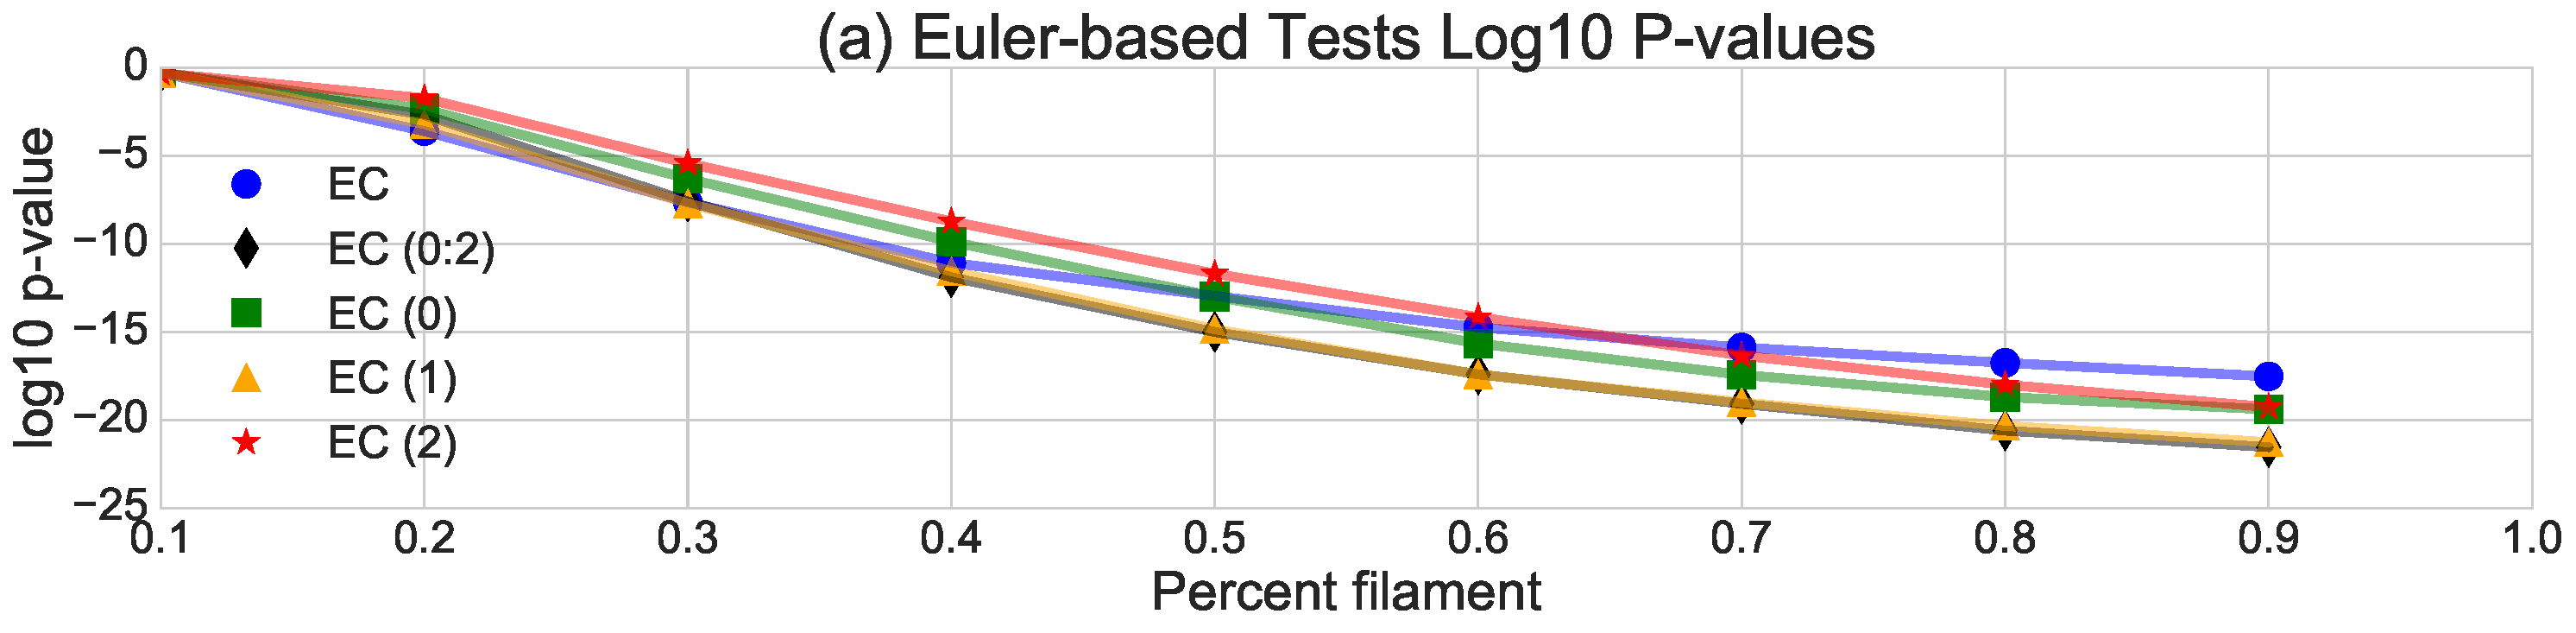
\includegraphics[width=0.7\linewidth]{euler_lineplot_log10_norm_False.pdf}
    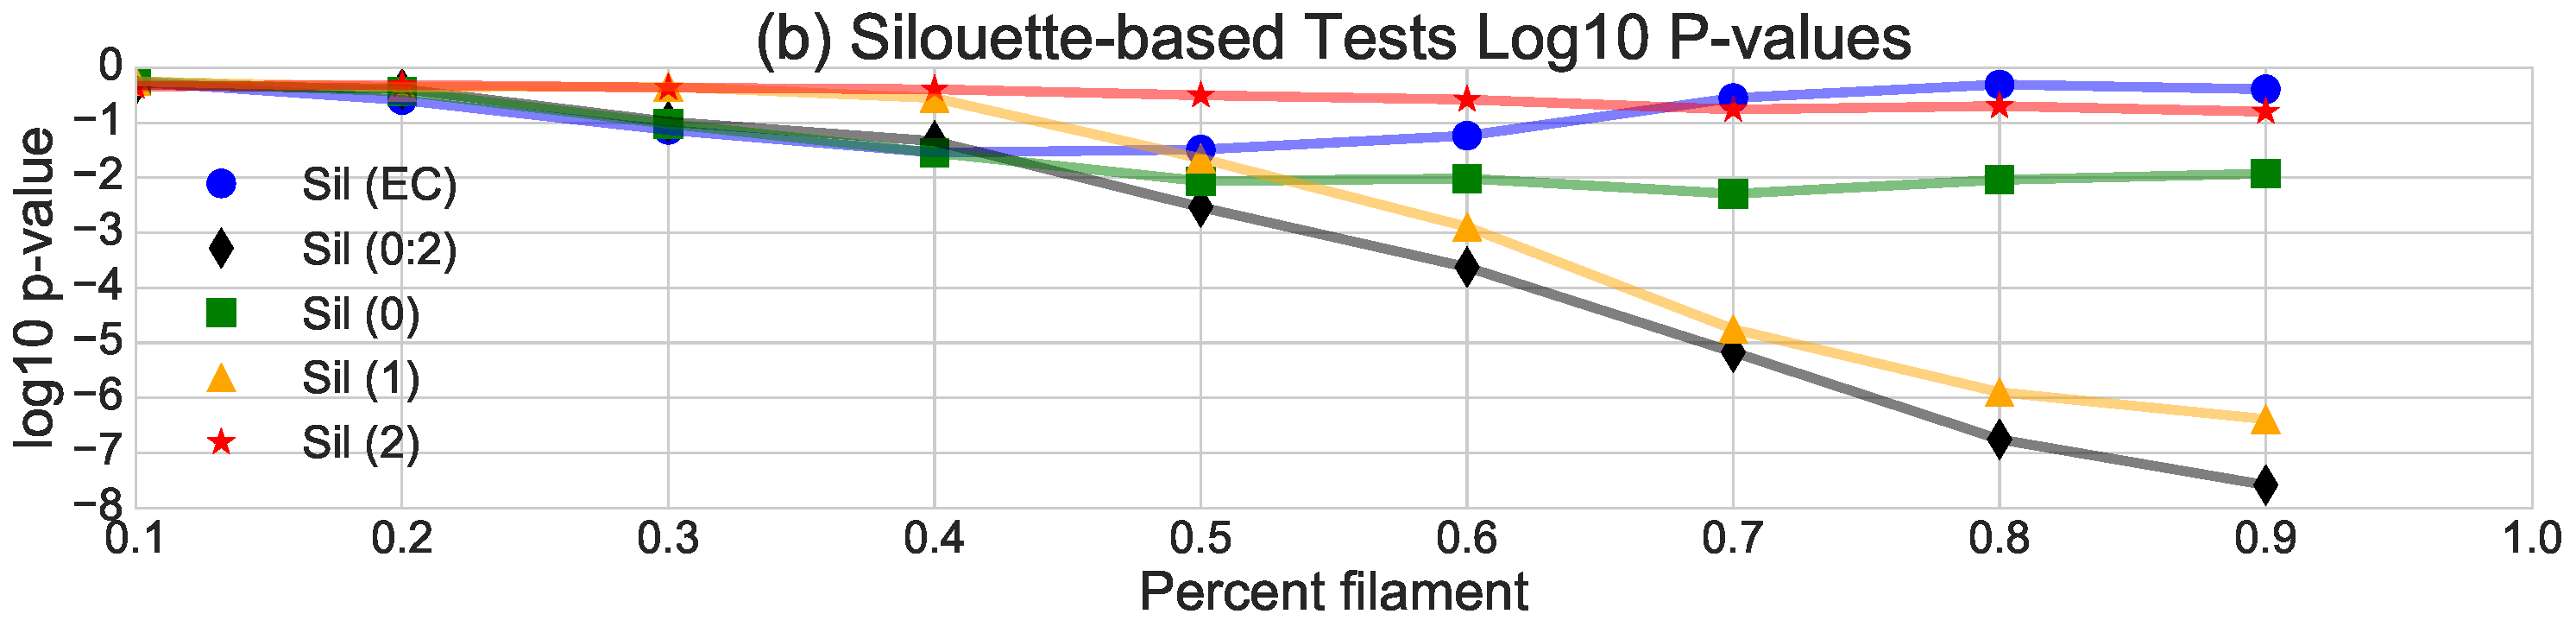
\includegraphics[width=0.7\linewidth]{silh_lineplot_log10_norm_False.pdf}
    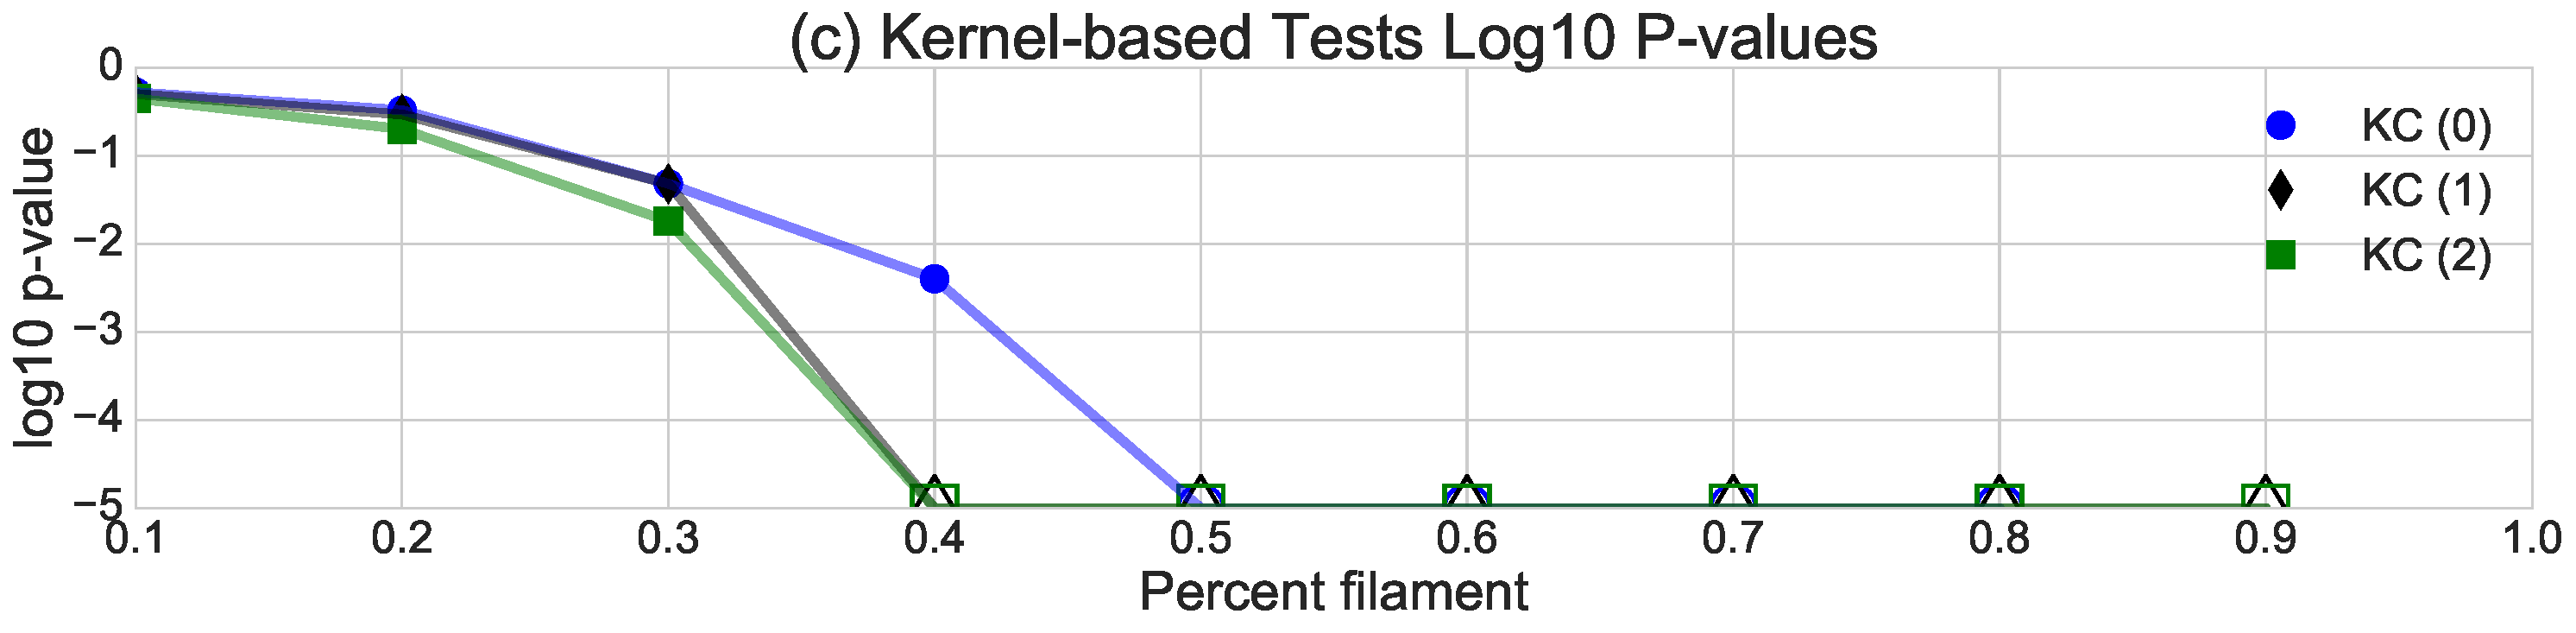
\includegraphics[width=0.7\linewidth]{smooth_lineplot_log10_norm_False.pdf}
    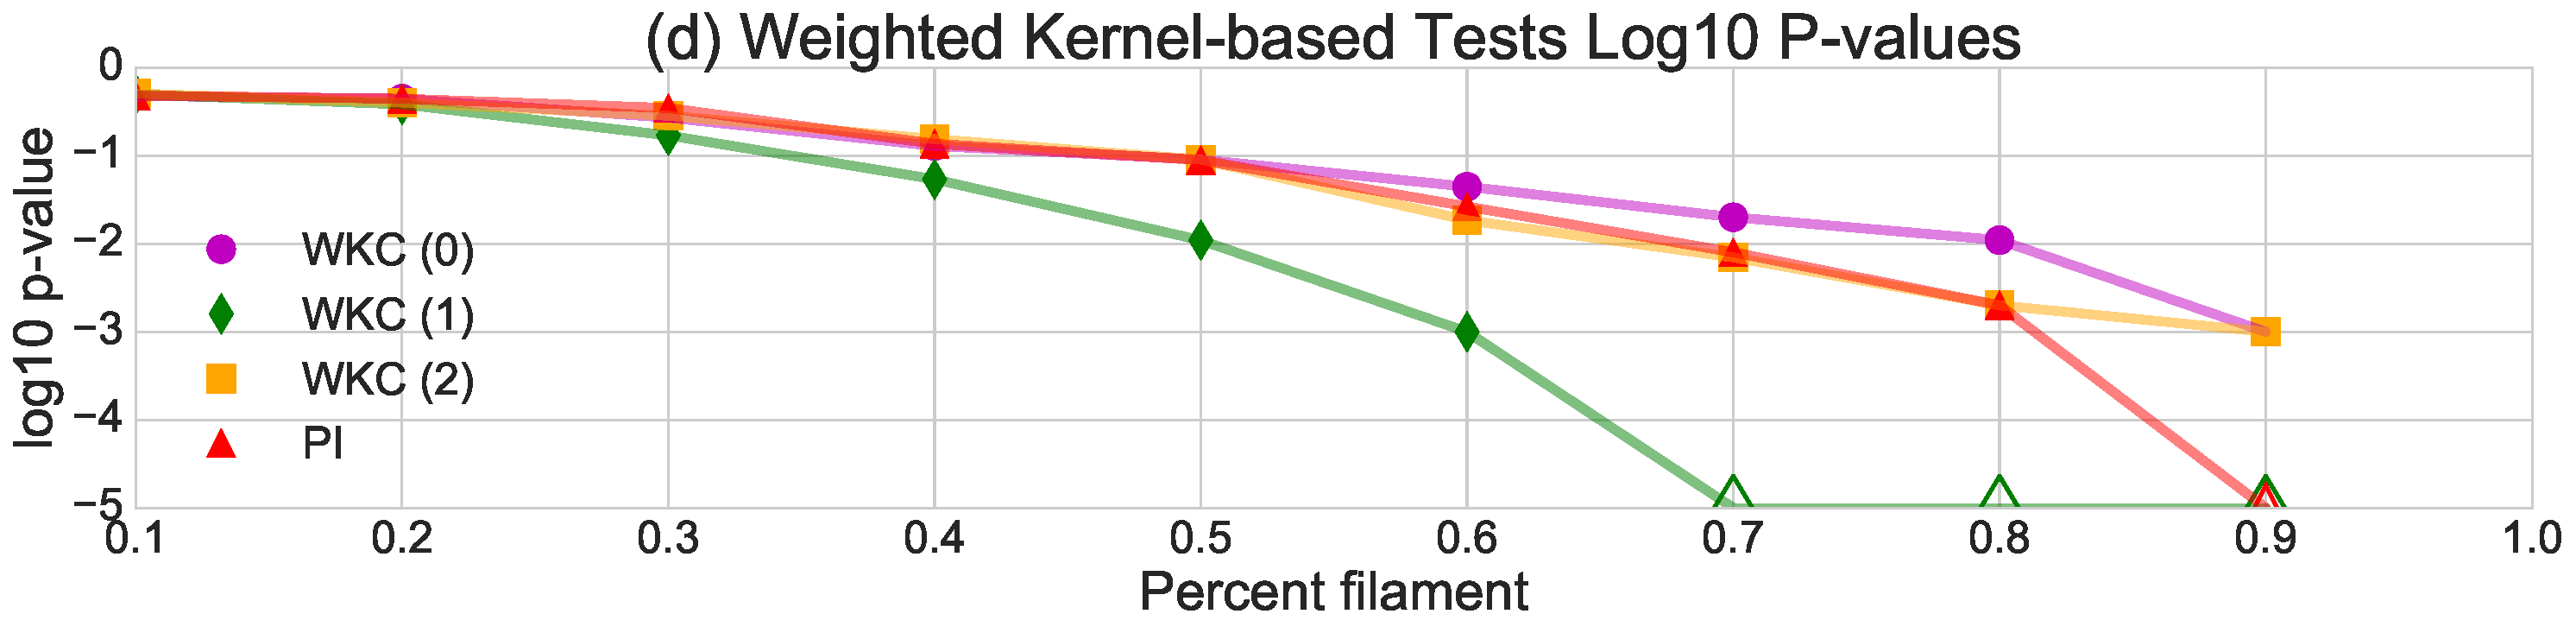
\includegraphics[width=0.7\linewidth]{weight_lineplot_log10_norm_False.pdf}
    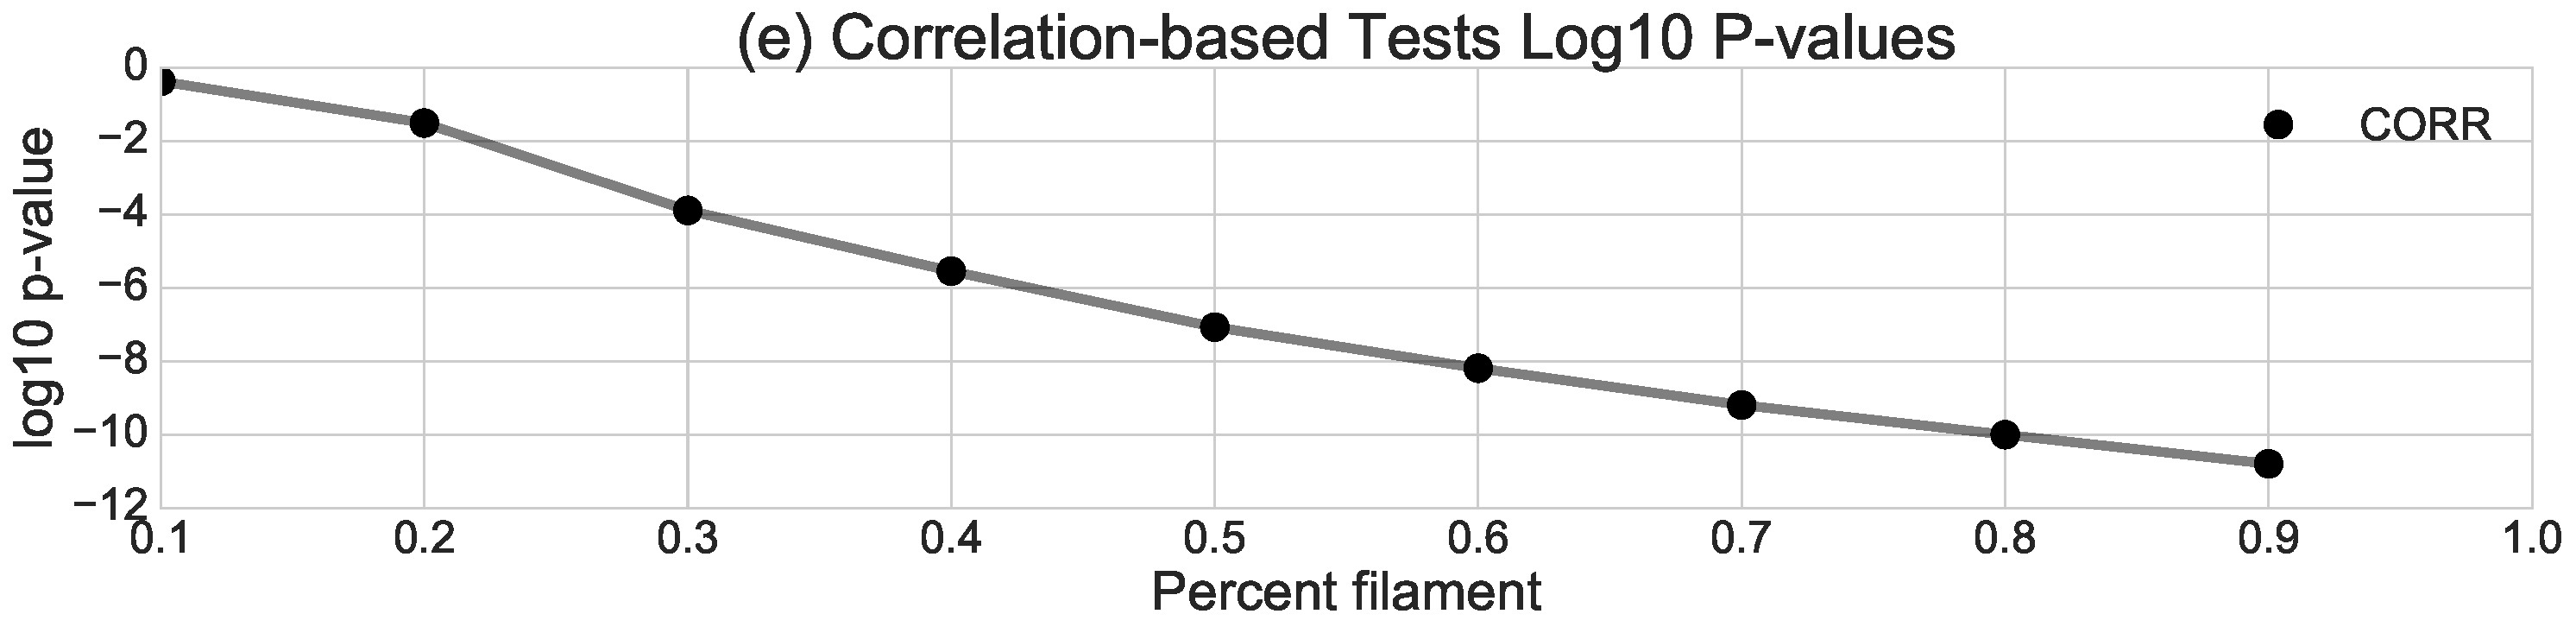
\includegraphics[width=0.7\linewidth]{corr_lineplot_log10_norm_False.pdf}
    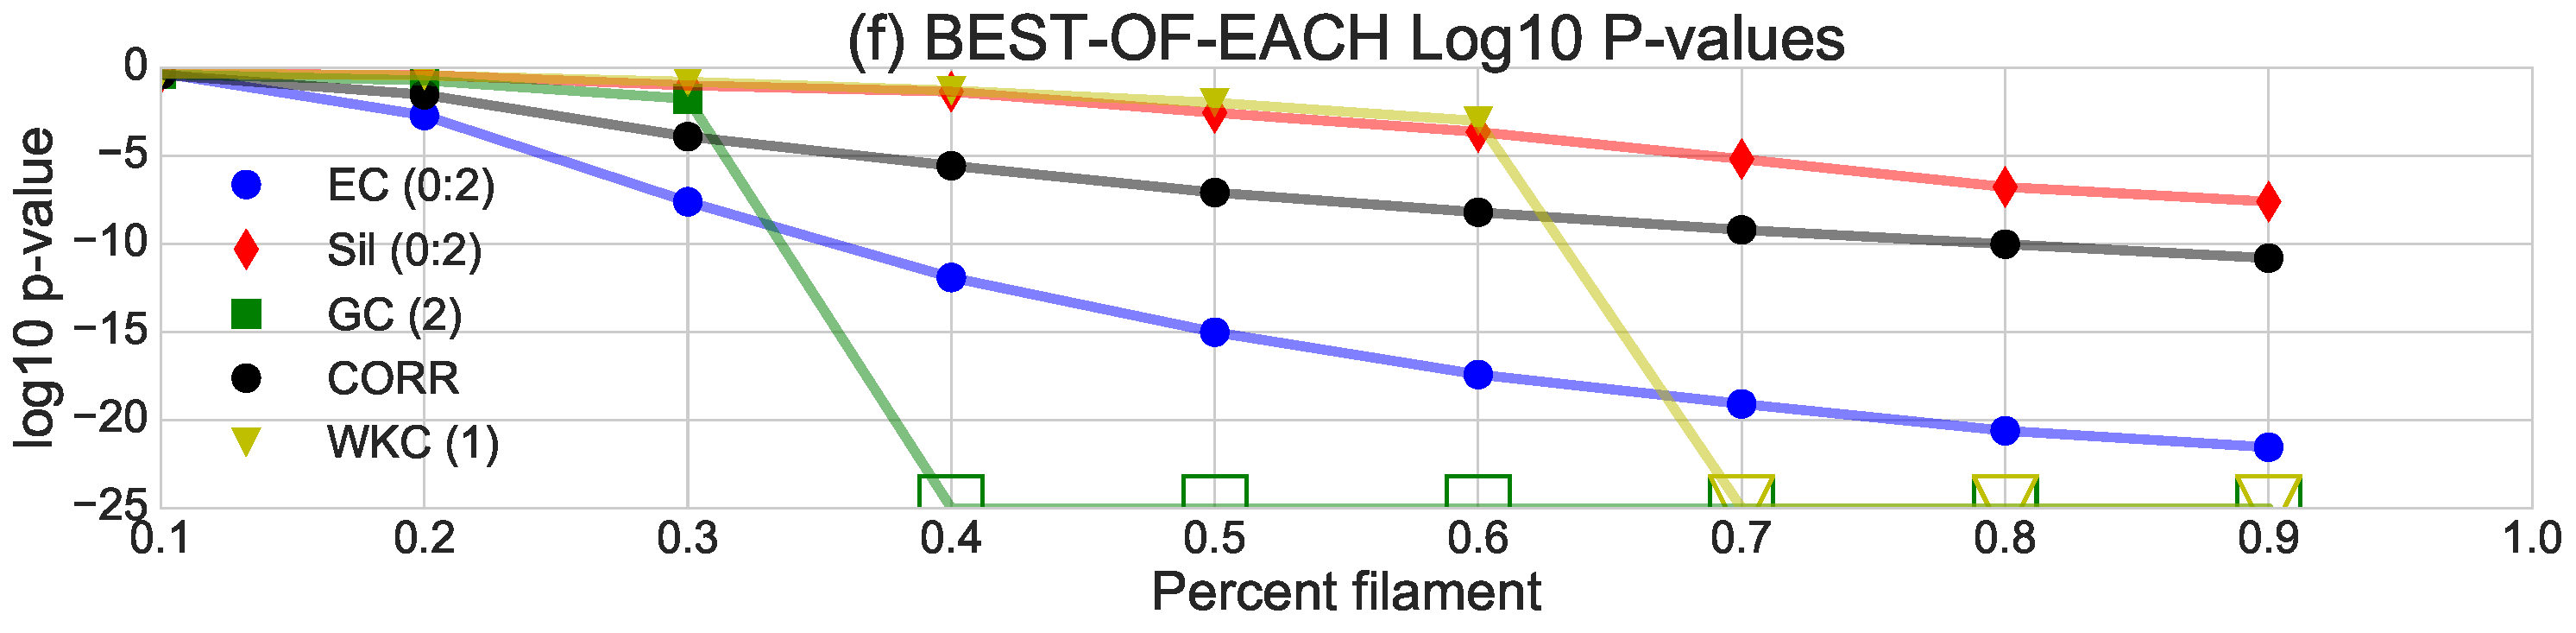
\includegraphics[width=0.7\linewidth]{cross_lineplot_log10_norm_False.pdf}
    \caption{$\log_{10}$ p-values for the proposed test statistics in the simulation study: (a) Euler-based, (b) Silhouette-based, (c) Kernel-based, (d) Weighted Kernel-based, (e) Correlation-based. The fifth plot (f) includes the best hypothesis test from each of three frameworks. X-axis represents the percent filament of the set being compared to the baseline set; y-axis shows the p-values in $\textup{1og}_{10}$ space. The lines plot the median $\log_{10}$ p-value of the 100 iterations. }
    \label{fig:linesUnnorm}
\end{figure}



{\color{red} Add a new discussion of the results here.} 

\subsubsection{Standardization of persistence diagrams} \label{sec:standardize}
Since the goal is to discern topological differences between two samples, issues with the proposed method is that scaling differences can result in rejection when, in fact there are not statistically significant topological differences.  For example, suppose we are considering two datasets - one has points randomly sampled from the perimeter of a circle with a radius of 1 and the other sample has points randomly sampled from the perimeter of a circle with a radius of 10.  Depending on one's goals, it may or may not be desirable to conclude that the two datasets come from different persistence diagram generators (i.e. conclude $\mathcal P^{(1)} \neq \mathcal P^{(2)}$) since the inference would be based on geometrical (scaling) differences rather than topological differences.  If the desire is to focus on topological differences (and remove the geometrical differences), we propose a possible preprocessing step.
Specifically, we standardize the persistence diagrams so that all the homological features are re-scaled to $[0, 1]\times[0,1]$.  This simple standardization takes the persistence diagram window and shrinks it or expands it to fill the $[0, 1]\times[0,1]$ window, maintaining the same relationship among all the homological features.  If there is concern about outliers, then other quantiles (rather than the minimum and maximum) could be used for the standardization.

We repeated the simulation study from Section~\ref{sec:results1} except included the standardization step noted above; the results are displayed in Figure~\ref{fig:linesNorm}.
Standardization had an appreciable impact on hypothesis test results, decreasing the effectiveness of several test statistics. Notice, however, that the best-performing test statistics remain the same as those from the unstandardized setting. 
{\color{red} add a new discussion on this part.} 

\begin{figure}[htp!]
  \centering
  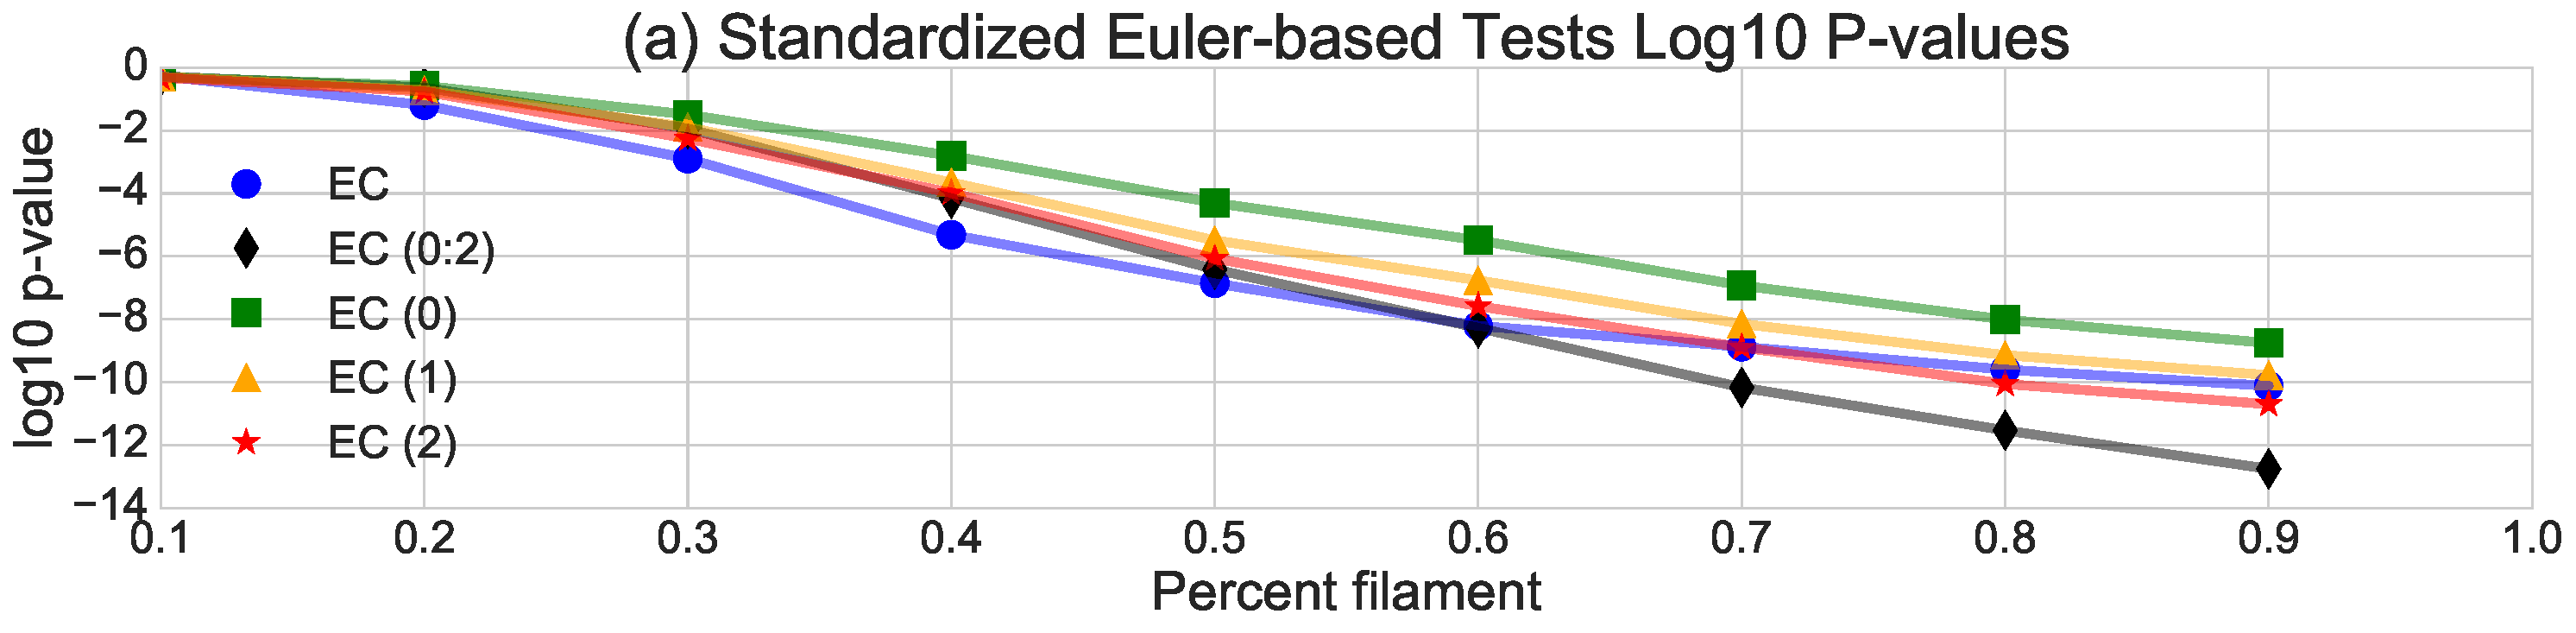
\includegraphics[width=0.7\linewidth]{euler_lineplot_log10_norm_True.pdf}
    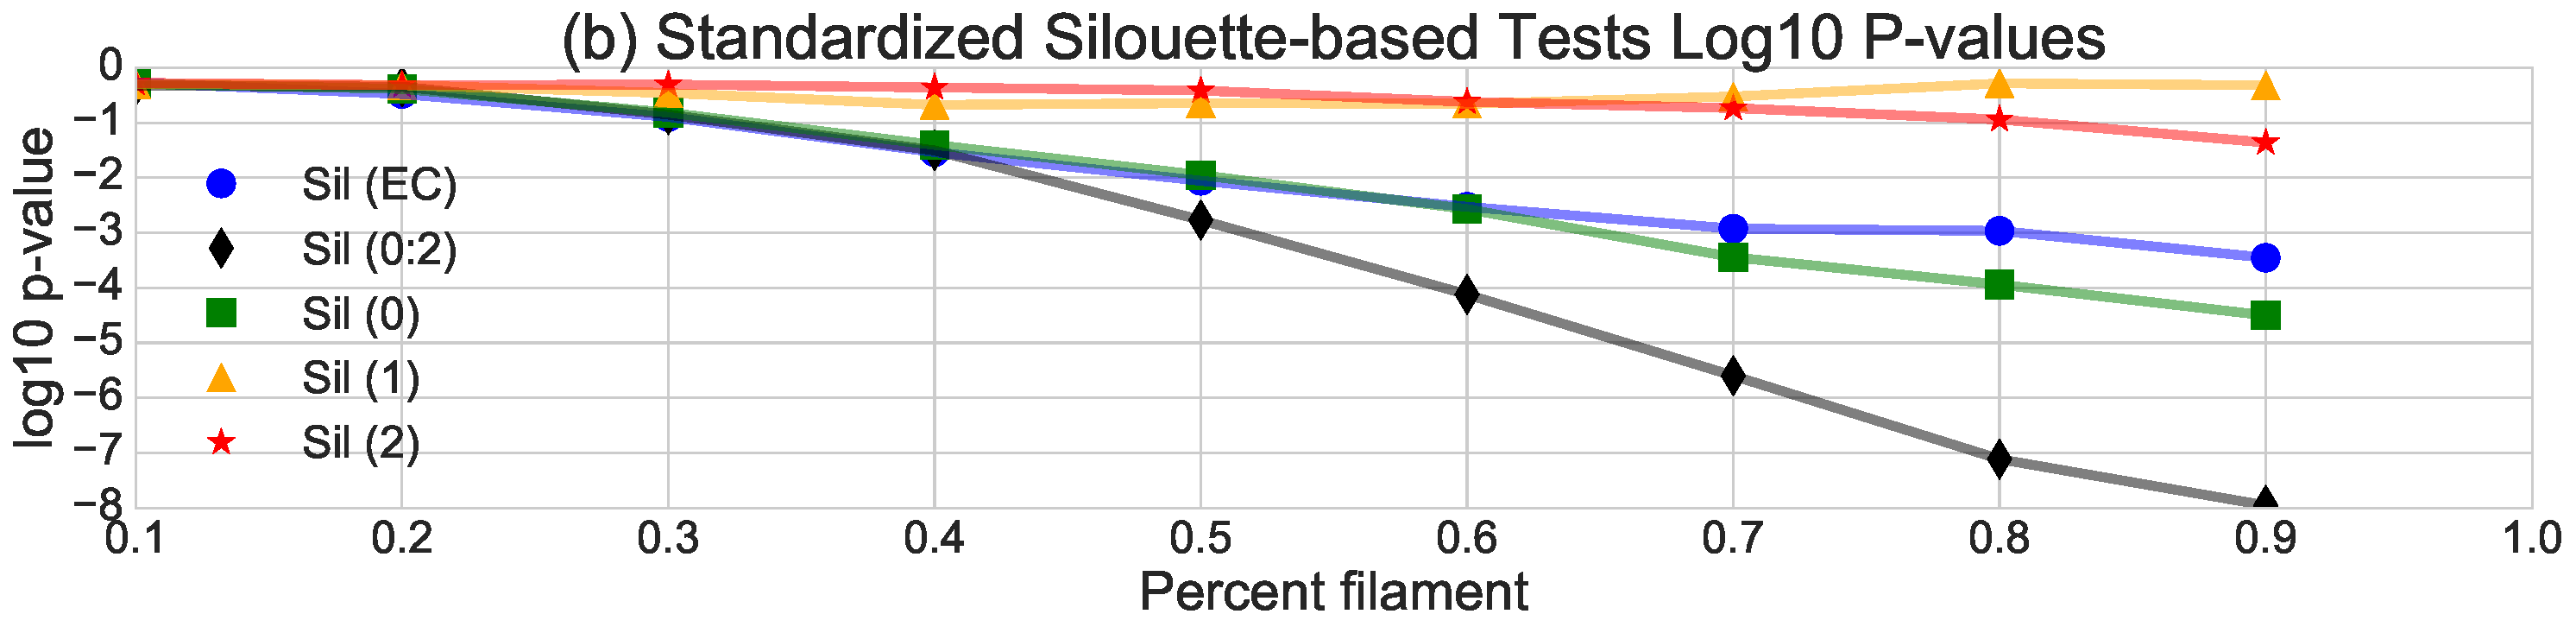
\includegraphics[width=0.7\linewidth]{silh_lineplot_log10_norm_True.pdf}
    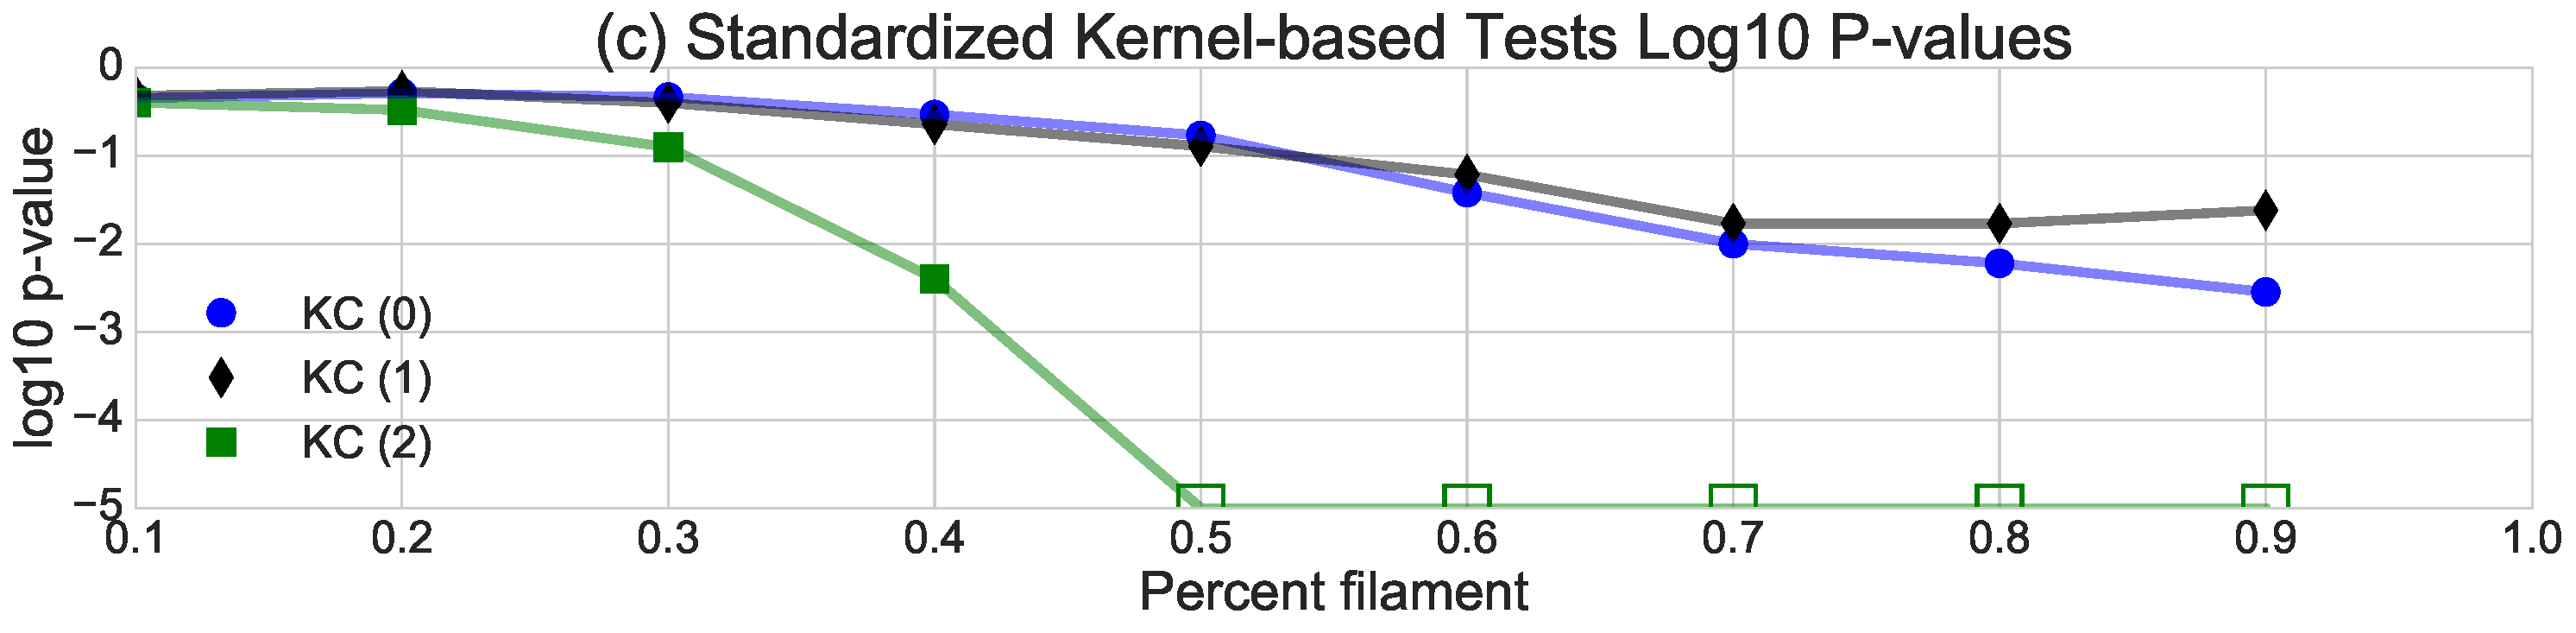
\includegraphics[width=0.7\linewidth]{smooth_lineplot_log10_norm_True.pdf}
    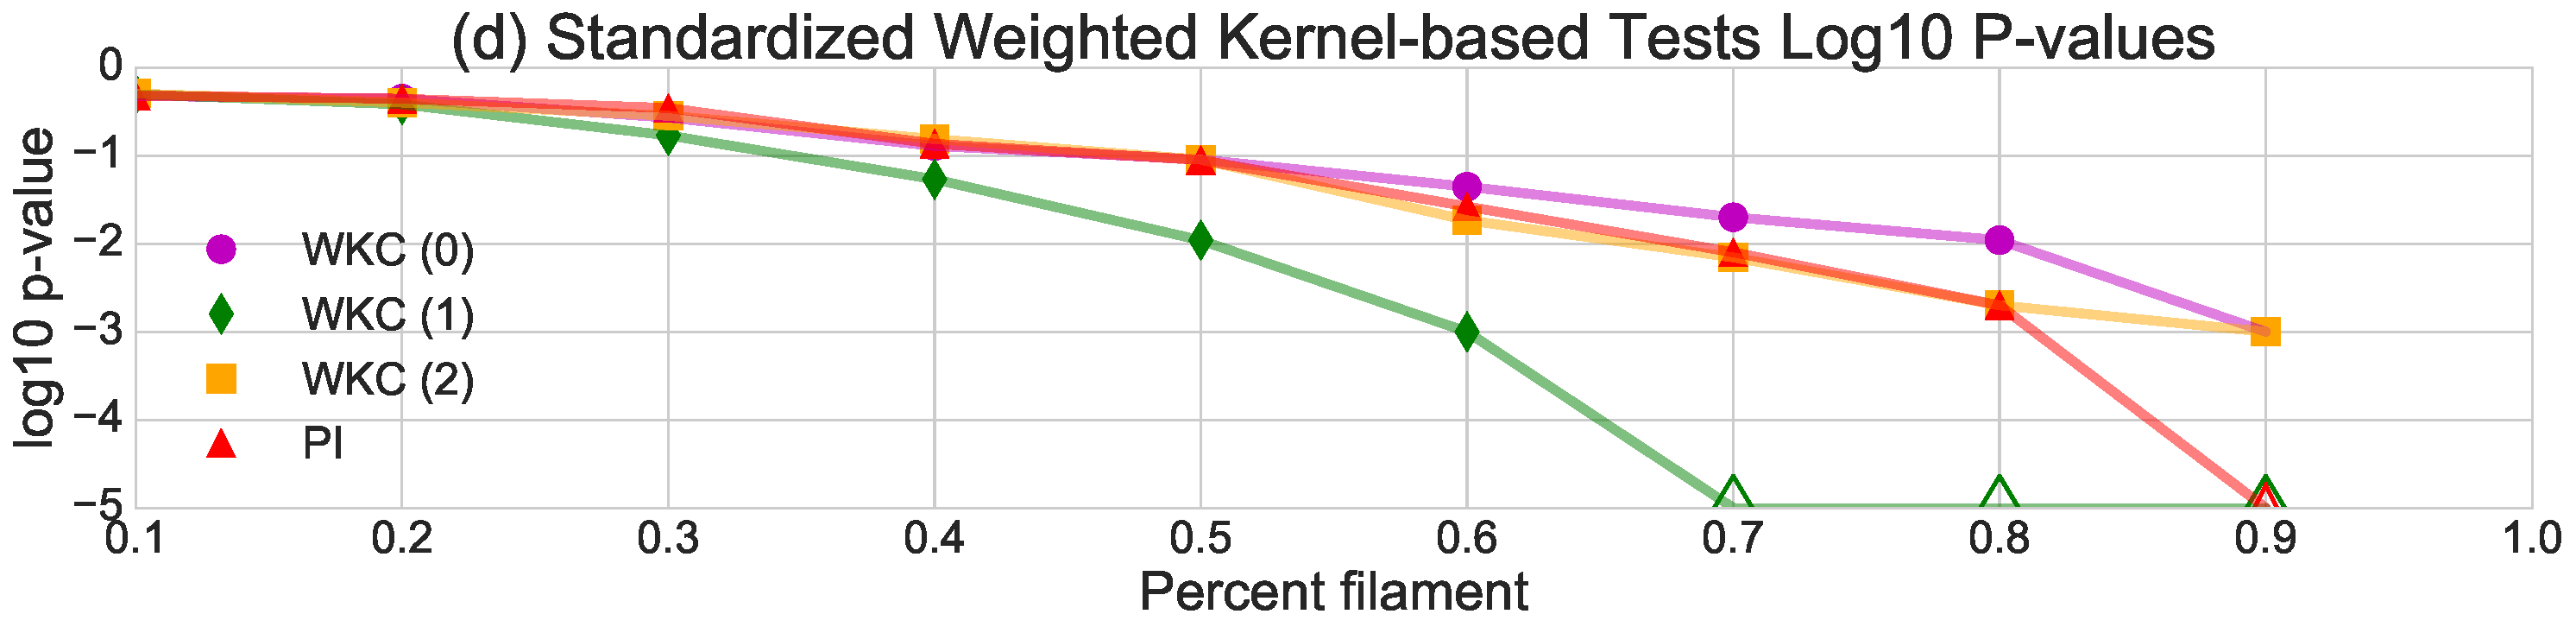
\includegraphics[width=0.7\linewidth]{weight_lineplot_log10_norm_True.pdf}
    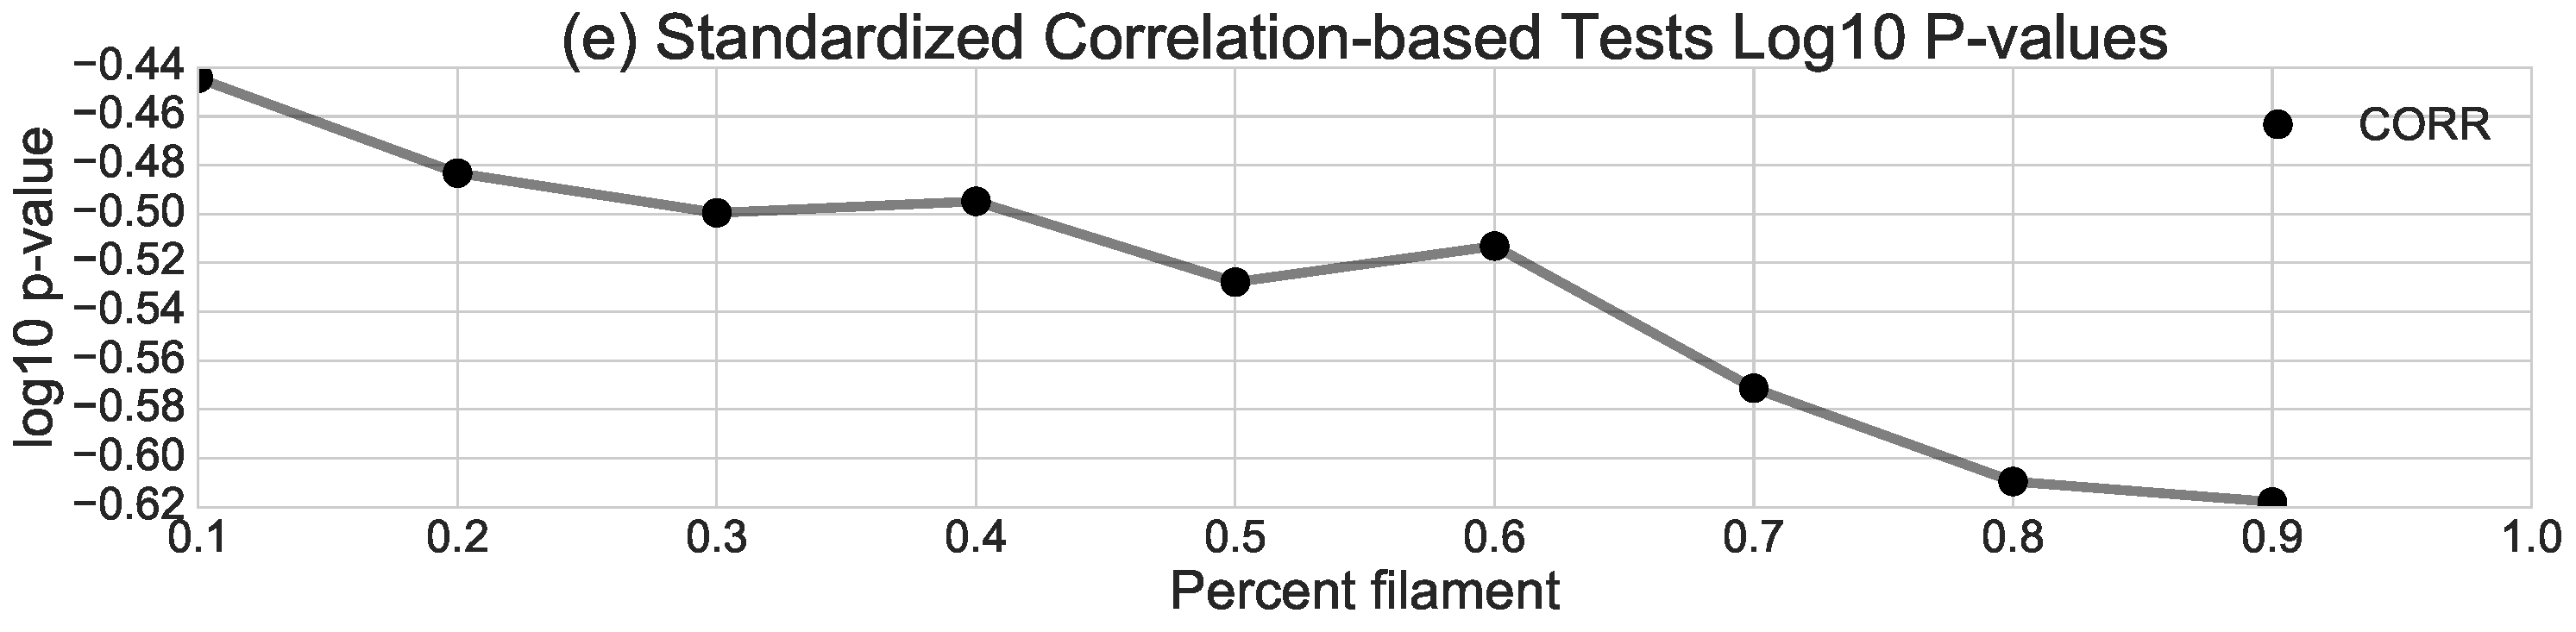
\includegraphics[width=0.7\linewidth]{corr_lineplot_log10_norm_True.pdf}
    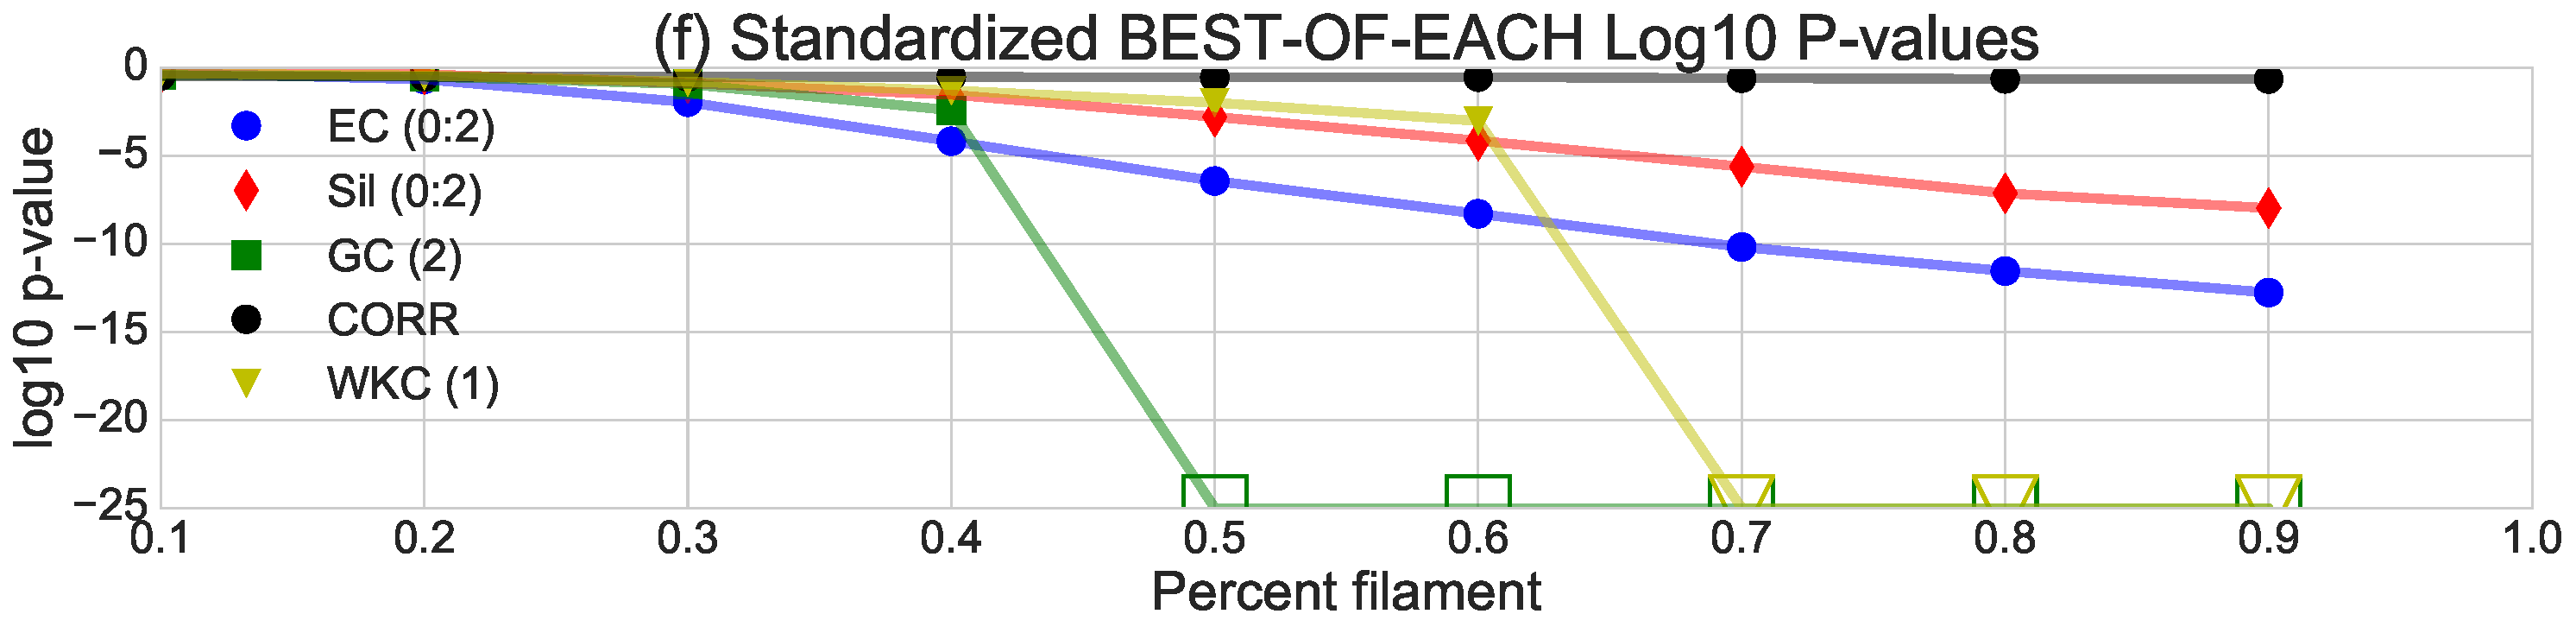
\includegraphics[width=0.7\linewidth]{cross_lineplot_log10_norm_True.pdf}
    \caption{Line plots of four classes of hypothesis testing frameworks: (a) Euler-based, (b) Silhouette-based, (c) Kernel-based, (d) Weighted Kernel-based, (e) Correlation-based. The fifth plot (f) includes the best hypothesis test from each of three frameworks. All axes were standardized prior to hypothesis testing.}
    \label{fig:linesNorm}
\end{figure}

%%%%%%%%%%%%%%%%%%%%%%%%%%%%%%%%%%%%%%%%%%%%%%%%%%%%%%%
%% SECTION: APPLICATION
%%%%%%%%%%%%%%%%%%%%%%%%%%%%%%%%%%%%%%%%%%%%%%%%%%%%%%%

\section{Application: Cosmological Simulation Data}
\label{sec:application}

Similar to the simulation models from Section~\ref{sec:sim_model}, the Megaparsec cosmic mass distributions are likewise characterized by intricate multiscale configuration of web-like filaments and voids.  We apply the proposed methodology to cosmological simulation data.

\begin{itemize}
\item  Discuss LSS
\item  Discuss Cosmological simulations
\item  Discuss Warm vs. Cold DM
\end{itemize}
Real observations of cosmic web:  Great Wall \cite{geller1989mapping}, Sloan Great Wall \cite{gott2005map}, gas \cite{cantalupo2014cosmic}.

We analyze N-body simulations of structure formation. The simulation box is 100 comoving Mpc on a side, and the numerical integration of the gravitational forces is run from redshift 127, when the age of the Universe is $<<$ 10Myr,  to the present day (13.8 Gyr).  The cosmological parameters are consistent with the 7-year results from the WMAP satellites: matter density $\Omega_0 = 0.272$, dark energy density $\Omega_{\Lambda} = 0.728$, Hubble parameter $h_0 = 0.704$, spectral index $n_s=0.967$, and power spectrum normalization $\sigma_8=0.81$. The mass of the simulation particle is $8.8x10^6$ $M_{sun}$. Haloes and subhaloes were identified using the SUBFIND algorithm {\color{red} Springel2001}, and the smallest halo that can be resolved has 20 particles. These runs were performed to be dark matter-only counterparts to the the hydrodynamical runs of the Eagle project \cite{schaye2015eagle}; we stress that the runs used in this paper use gravity alone. 

We use two simulations in this study, one cold dark matter (CDM) and the other warm dark matter (WDM) (recall Figure~\ref{fig:introData}). They make use of the same initial phases, and differ in that the latter has wave amplitudes rescaled using the transfer function of a 3.3keV thermal relic, the relic mass chosen to be in agreement with the Lyman-alpha constraints of \cite{viel2013warm}. This results in the suppression of structure on the scale of dwarf galaxies. Spurious subhaloes have been removed using the algorithm of \cite{lovell2014properties}.

In the simulation study, all test were standard two-sample T-tests  using the varying proposed test statistics derived from the persistence diagrams.  For our two cosmological simulation cubes, one might consider cutting up the cubes into sub-cubes to produce similar sets of samples used in the voronoi experiments. Let a \textit{double-split} be defined as splitting the simulation cube along both the $x$ and $y$ axis into $2$ equal groups, creating 4 equally sized cubes in total. \textit{quadruple-split} are defined in a similar fashion, producing 64 equally sized cubes, further splitting each of the cubes in a \textit{double-split} set into four sub-cubes. Using this splitting technique on both the CDM and WDM simulations, we end up with two usable data sets. By doing this, however, the WDM and CDM data sets are correlated due to their identical initial conditions.  That is, the differences between the two cosmological simulation cubes is due to differences in the physics of warm vs. cold DM.  Because of this, the skeleton structure of the warm and cold DM simulations are nearly identical, allowing for paired T-tests.  Note that there is also correlation between the samples due to the large-scale structure crossing the boundaries of the sub-cubes.  We investigate this by changing the sizes of the sub-cubes, but consequently by doing so, decreases our sample size.

\begin{figure}[htp!]
  \centering
  \begin{subfigure}{0.25\textwidth}
    \centering
        \caption{}
  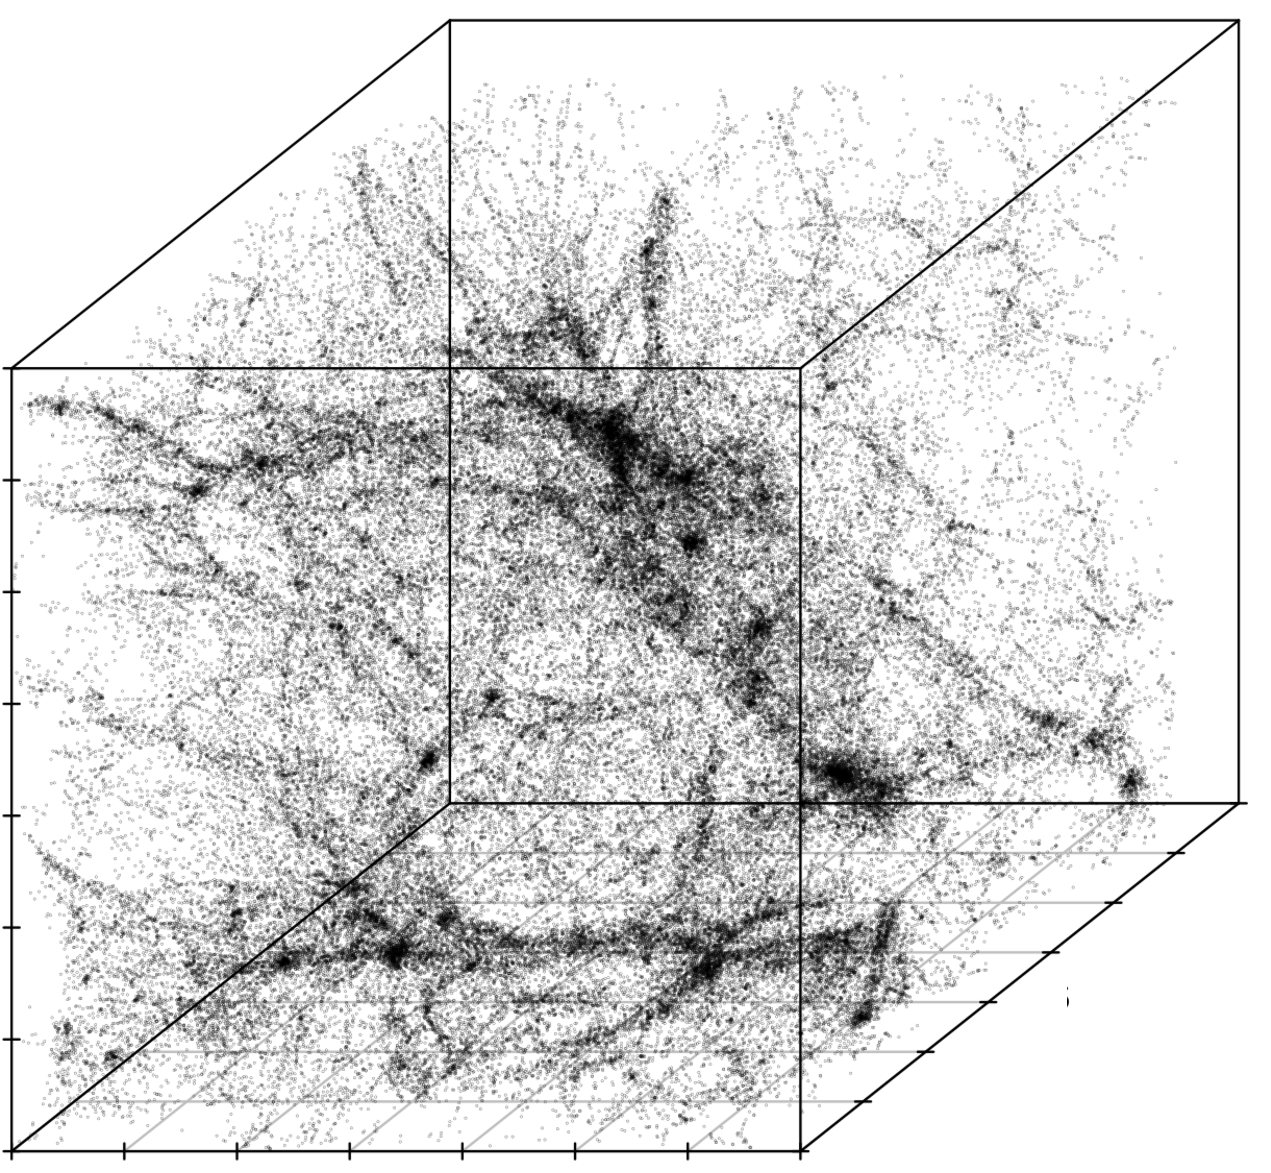
\includegraphics[width=\linewidth]{triplesplitA.pdf}
    \label{fig:cubeDiagsA}
  \end{subfigure}
    \begin{subfigure}{0.25\textwidth}
    \centering
        \caption{}
  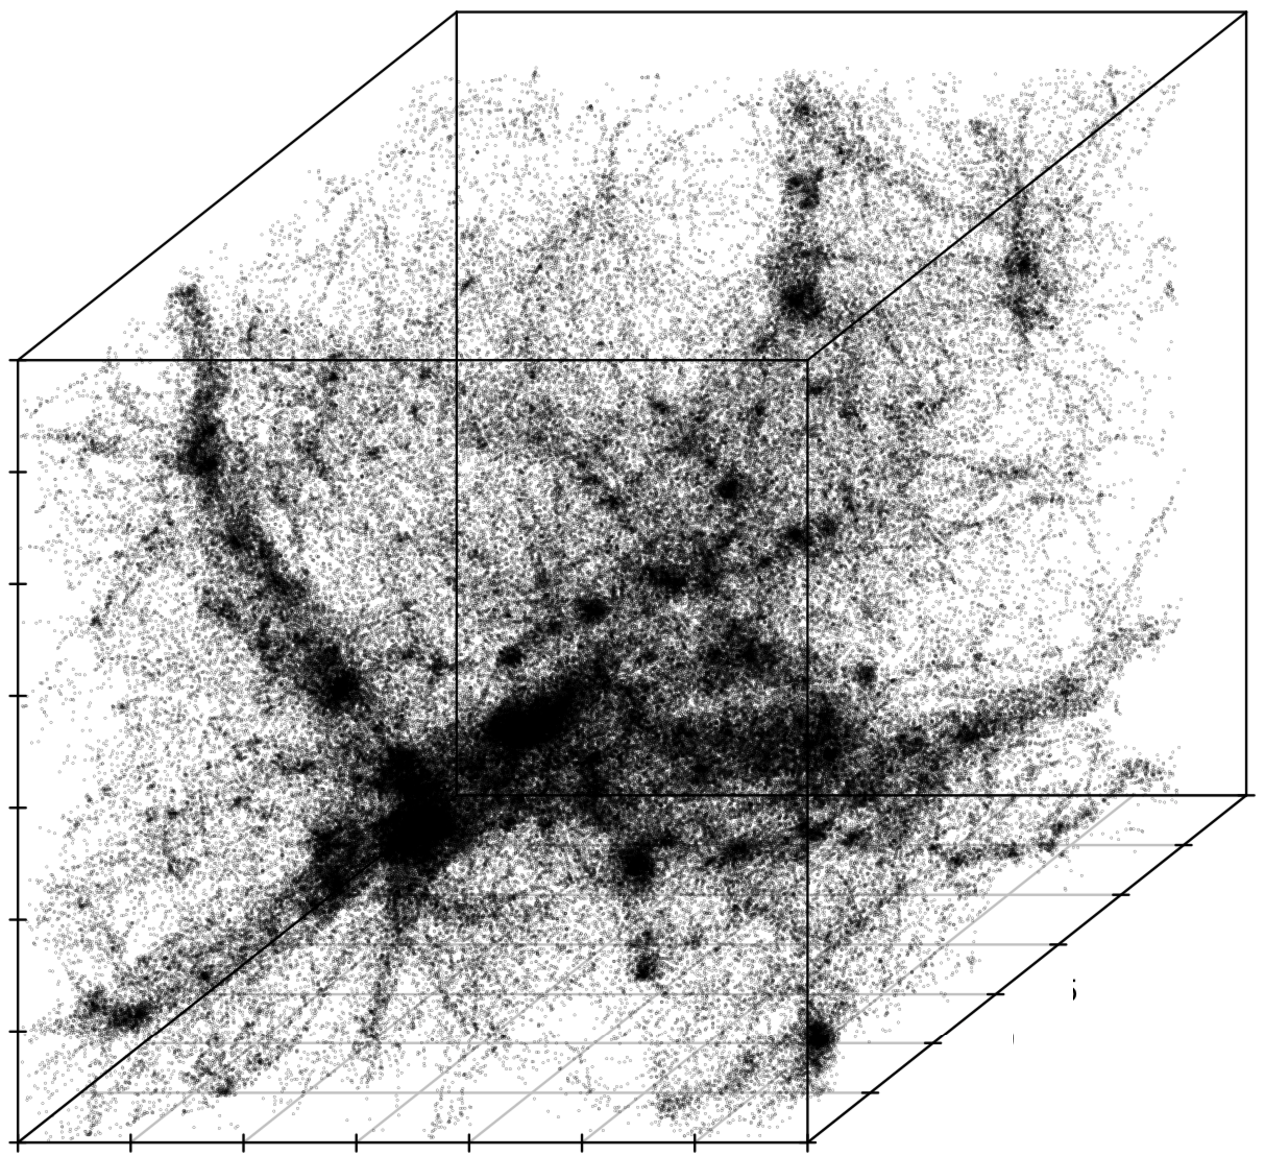
\includegraphics[width=\linewidth]{triplesplitB.pdf}
    \label{fig:cubeDiagsB}
  \end{subfigure}
    \begin{subfigure}{0.25\textwidth}
    \centering
        \caption{}
  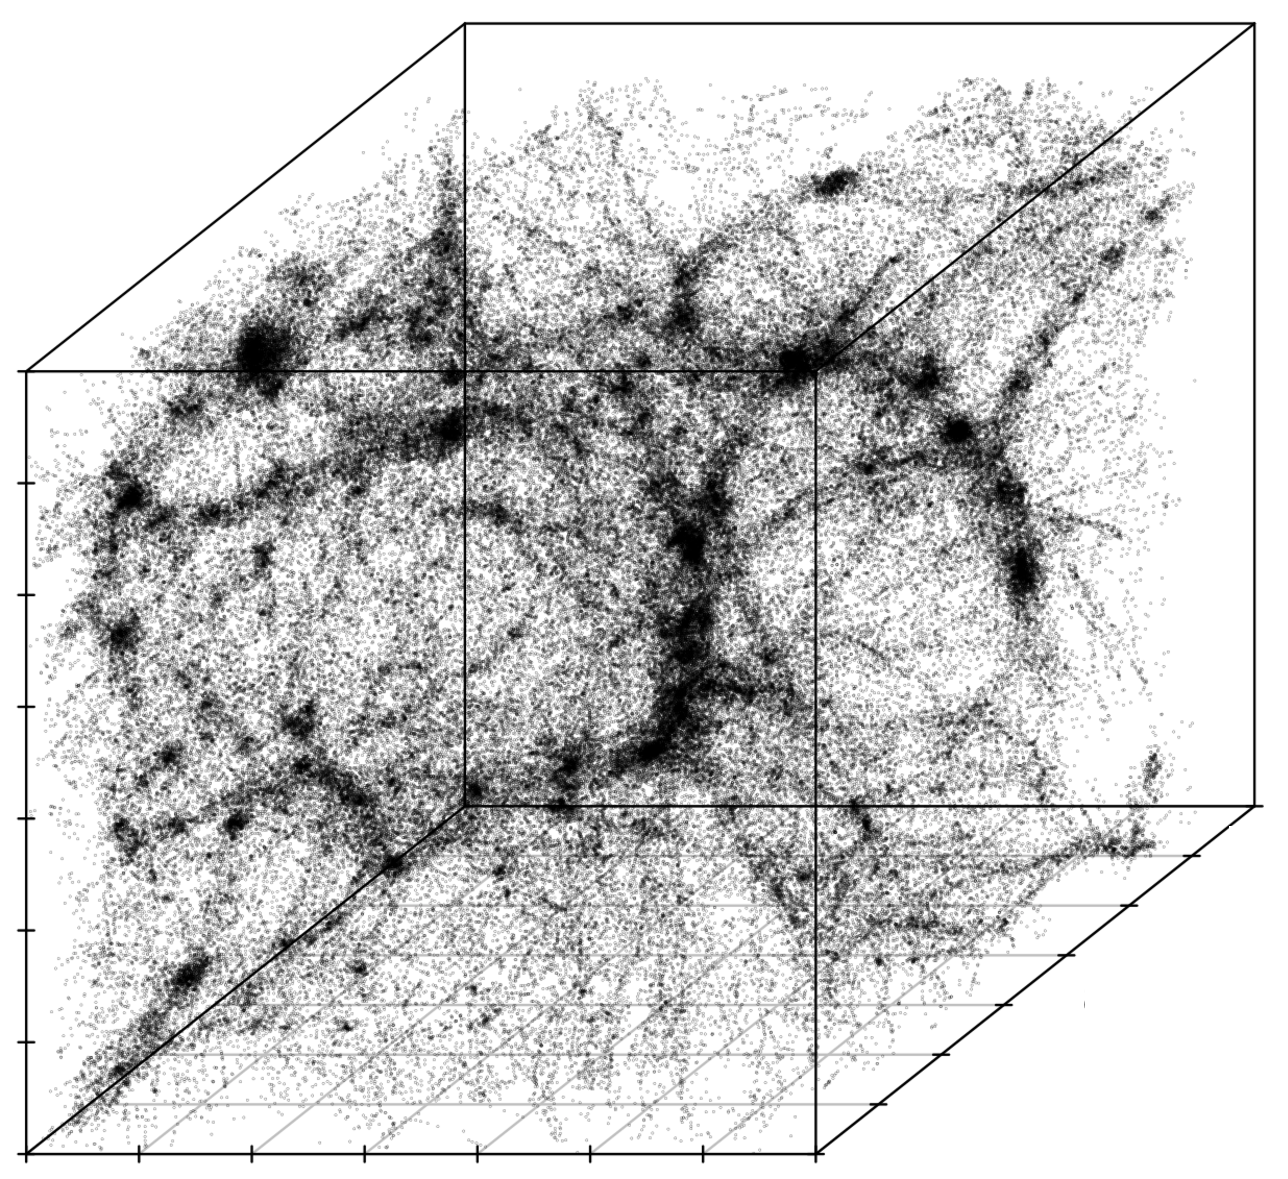
\includegraphics[width=\linewidth]{triplesplitC.pdf}
    \label{fig:cubeDiagsC}
  \end{subfigure}
    \caption{Examples of three triple-split samples from a CDM simulation.}
    \label{fig:cubeDiags}
\end{figure}

% Using the proposed method, we study simulations of the Megaparsec cosmic mass and evaluate similarities and differences in LSS based on variations in the parameters of the simulation. One particular parameter that we are interested in is the state of the dark matter in the simulation. Warm dark matter (WDM) and cold dark matter (CDM) are traditionally believed to produce very different realizations of the observable Universe, with the latter involving more slowly moving particles prone to produce a more lumpy distribution of galaxies and clusters in the LSS. The former, containing more kinetic energy, has higher resistance to formation of global structure, and is theorized to render a less topologically-interesting cosmic mass. Applying the proposed hypothesis testing framework would offer a method to \emph{quantify} the topological differences between simulations with underlying WDM and CDM assumptions.

\subsection{The EAGLE project}
We analyze N-body simulations of structure formation. The simulation box is $100$ co-moving Mpc on a side, and the numerical integration of the gravitational forces is run from redshift $127$, when the age of the Universe is much less than $10$ Myr,  to the present day ($13.8$ Gyr). The cosmological parameters are consistent with the seven year results from the WMAP satellites: matter density $\Omega_0 = 0.272$, dark energy density $\Omega_{\Lambda} = 0.728$, Hubble parameter $h0 = 0.704$, spectral index $n_{s}=0.967$, and power spectrum normalization $\sigma_8=0.81$. The mass of the simulation particle is $8.8 \times 10^{6}$ Msun. Haloes and subhaloes were identified using the SUBFIND algorithm \cite{springel2001populating}, and the smallest halo that can be resolved has $20$ particles. These runs were performed to be dark matter-only counterparts to the the hydrodynamical runs of the EAGLE project \cite{schaye2015eagle}; we stress that the runs used in this paper use gravity alone. 

\begin{figure}[htp!]
  \centering
  \label{fig:eagleDiags}
  \begin{subfigure}{0.24\textwidth}
        \caption{Eagle CDM}
  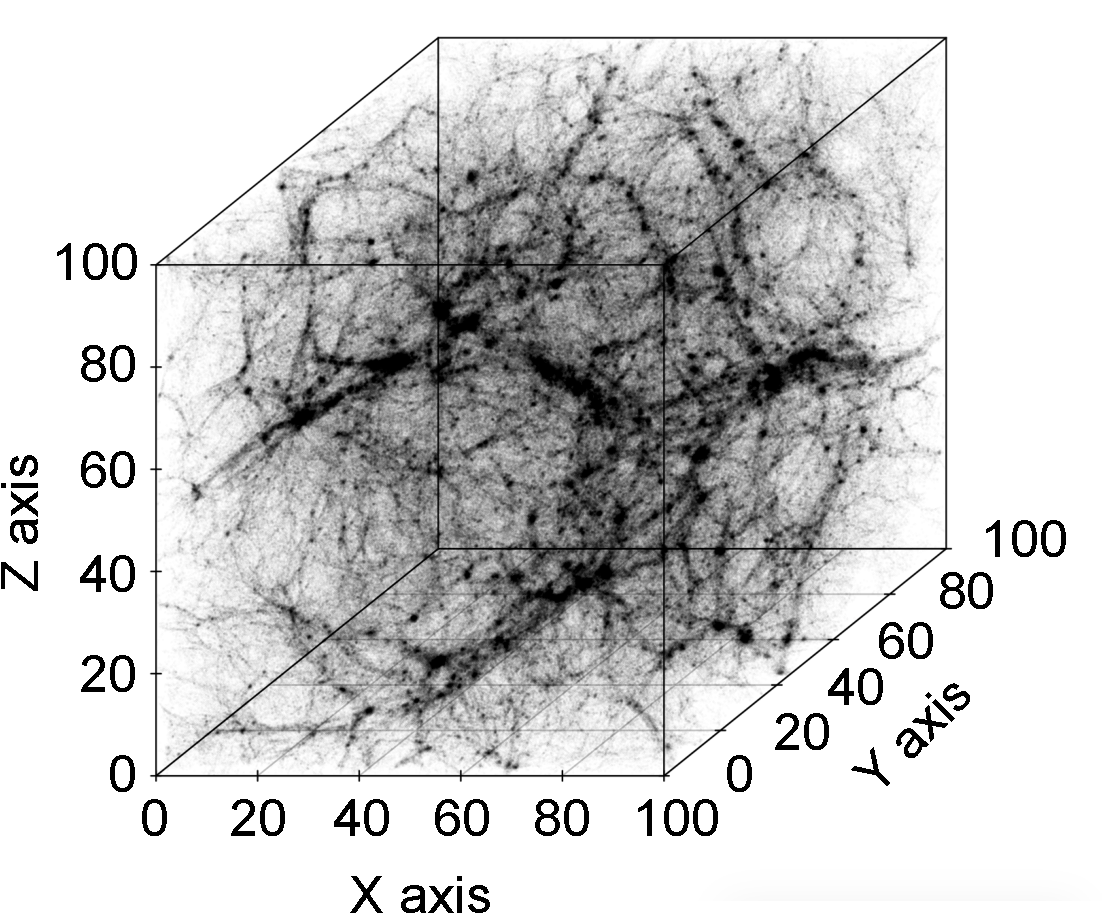
\includegraphics[width=\linewidth]{wdmfig.pdf}
    \label{fig:eagleDiagsA}
  \end{subfigure}
    \begin{subfigure}{0.24\textwidth}
        \caption{Eagle WDM}
  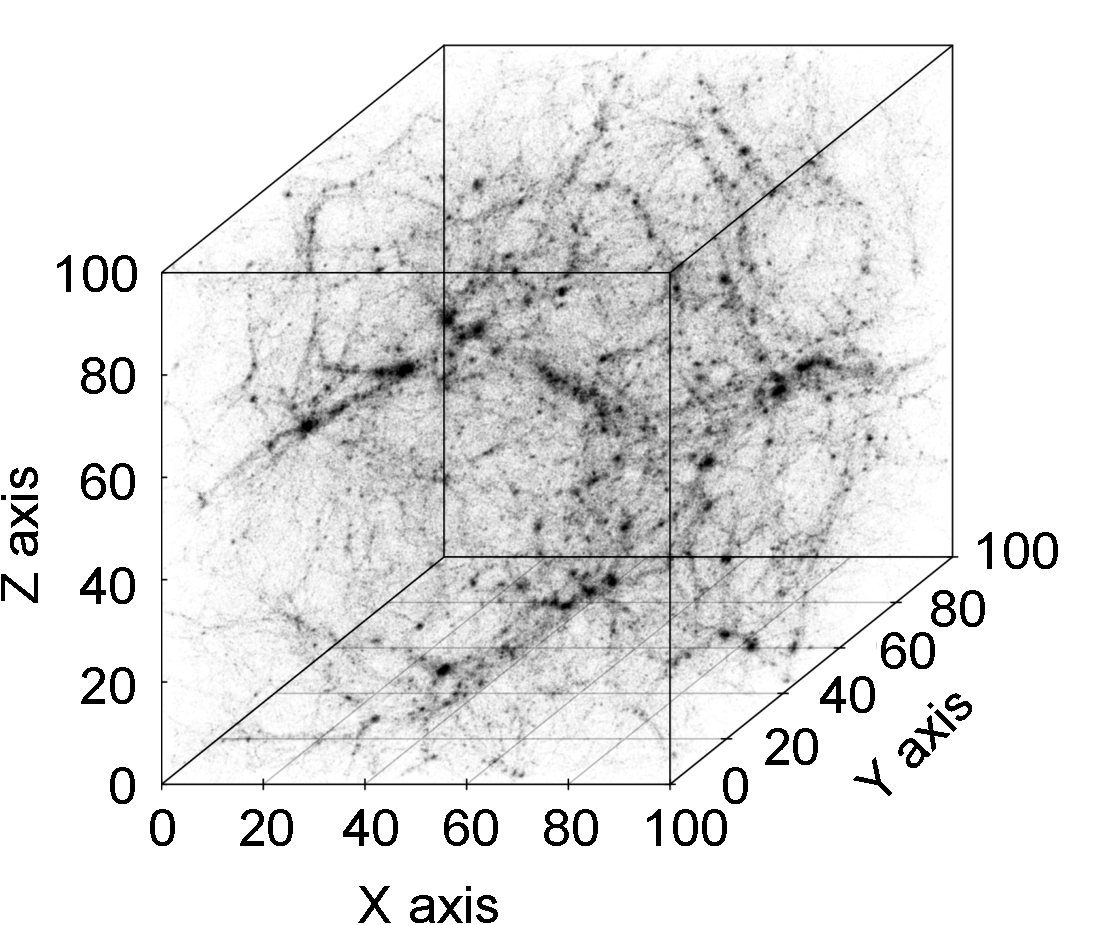
\includegraphics[width=\linewidth]{cdmfig.pdf}
    \label{fig:eagleDiagsB}
  \end{subfigure}
    \begin{subfigure}{0.24\textwidth}
    \caption{Eagle CDM PD}
  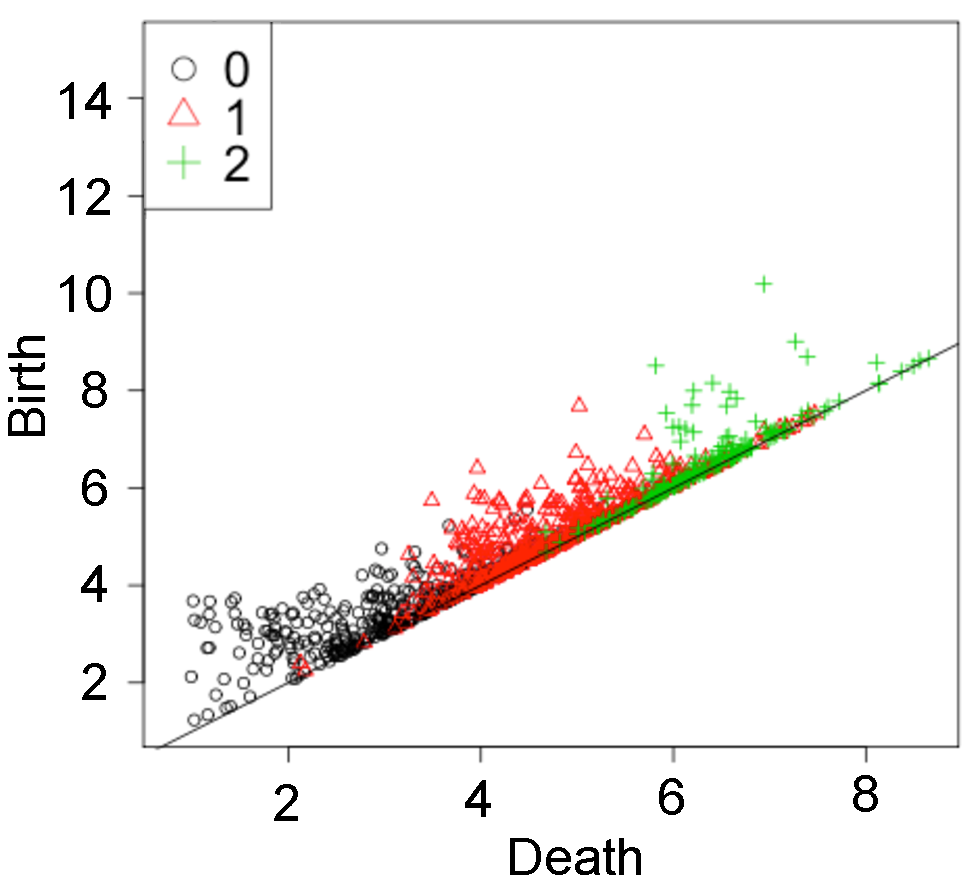
\includegraphics[width=\linewidth]{cdmdiag.pdf}
    \label{fig:eagleDiagsC}
  \end{subfigure}
    \begin{subfigure}{0.24\textwidth}
        \caption{Eagle WDM PD}
  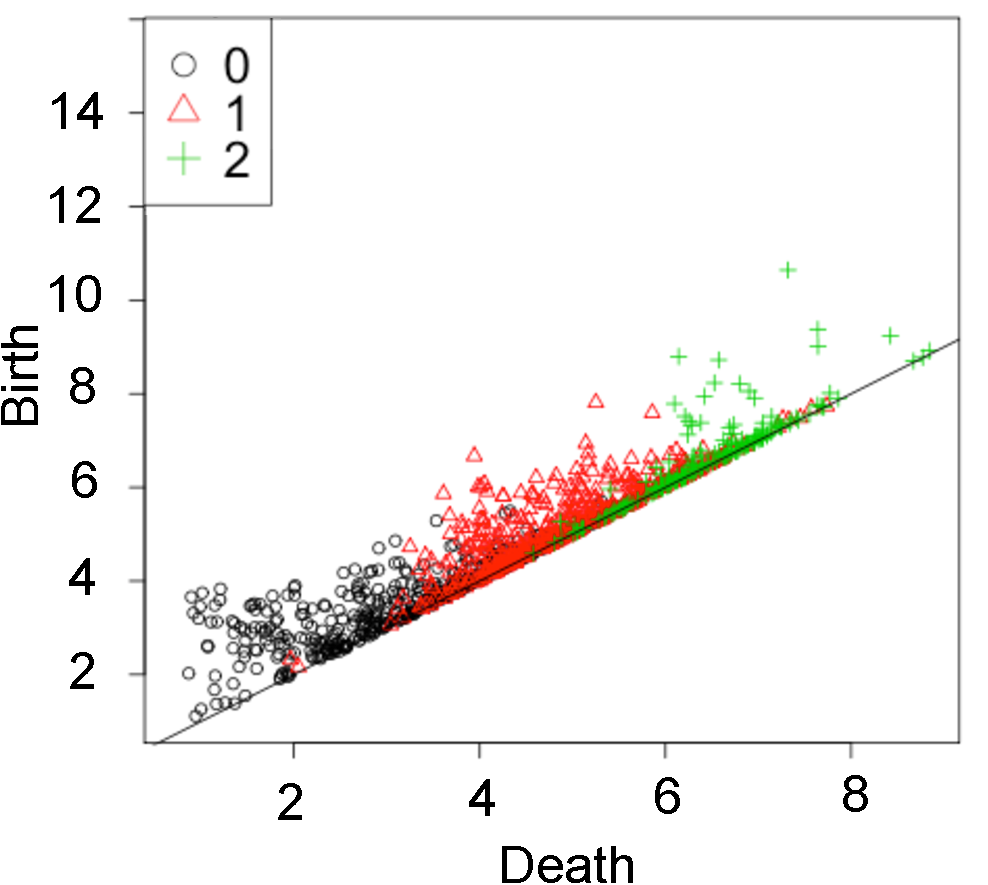
\includegraphics[width=\linewidth]{wdmdiag.pdf}
    \label{fig:eagleDiagsD}
  \end{subfigure}
    \caption{(a, b) Visualization of the complete CDM and WDM simulations. (c, d) Their corresponding persistence diagrams. Although the CDM structure is denser, the persistence diagrams appear comparable.} 
\end{figure}

We use two simulations in this study, one cold dark matter (CDM) and the other warm dark matter (WDM). They make use of the same initial phases, and differ in that the latter has wave amplitudes rescaled using the transfer function of a $3.3$ keV thermal relic, the relic mass chosen to be in agreement with the Lyman-alpha constraints of \cite{viel2013warm}. This results in the suppression of structure on the scale of dwarf galaxies. Spurious subhaloes have been removed using the algorithm of \cite{lovell2014properties}. Figure \ref{fig:eagleDiags} shows a scatter plot of both the CDM and WDM simulations along with their respective persistent diagrams. Visually, we can see that the CDM scatter plot is far more dense than WDM but share similar internal structure; the persistence diagrams also share a general structure but we can identify smaller differences in homology groups that we hope to quantify using the hypothesis testing framework. These diagrams were generated under a volume of $1\times 10^{6}$, resolution of $2$ and a DTM distance function with hyper-parameter $0.001$. 

\subsection{Results}
Having created datasets of multiple slices, the suite of hypothesis testing frameworks explored on Voronoi foams are applicable to the WDM and CDM data. Tables \ref{table:unnormhypoCDMWDMresults}, \ref{table:normhypoCDMWDMresults} shows both the standardized and unstandardized results of the five categories of hypothesis tests. The unstandardized results suggest the more splits, the more significant differences found in the topology. More interestingly still, a similar effect is observed through standardizing the persistence diagrams prior to hypothesis testing: all the frameworks produce higher p-values on average and are less confident in the difference between double-split and quadruple-split datasets. This seems to explain that similar to the Voronoi foams, a large degree of the topological difference between warm dark matter and cold dark matter assumptions in the large-scale universe are due to geometrical properties such as size.  

\begin{table}[htp!]
    \begin{center}
        \begin{tabular}{ l | c | c }
            Test & Double Split & Quadruple Split \\
            \hline
            EC & 1.156e-06 & 7.379e-26 \\
            $\textup{EC}_{0:2}$ & 2.104e-05 & 7.379e-28 \\
            $\textup{EC}_{0}$ & 3.273e-08 & 3.811e-30 \\
            $\textup{EC}_{1}$ &  1.849e-05 & 0.935 \\
            $\textup{EC}_{2}$ & 0.340 & 0.0877 \\
            \hline
            $\textup{Sil}_{\textup{EC}}$ & 7.709e-08 & 2.455e-20 \\ 
            $\textup{Sil}_{0:2}$ & 1.892e-06 & 1.114e-33 \\
            $\textup{Sil}_{0}$ & 2.958e-08 & 1.489e-34 \\
            $\textup{Sil}_{1}$ & 1.169e-05 & 2.884e-23 \\
            $\textup{Sil}_{2}$ & 0.925 & 0.0345 \\
            \hline
            $\textup{KC}_{0}$ & 0.442 & 0.000 \\
            $\textup{KC}_{1}$ & 0.192 & 0.000 \\
            $\textup{KC}_{2}$ & 0.248 & 0.00199 \\
            \hline
            $\textup{WKC}_{0}$ & 0.084 & 0.000 \\
            $\textup{WKC}_{1}$ & 0.051 & 0.000 \\
            $\textup{WKC}_{2}$ & 0.496 & 0.000 \\
            $\textup{PI}$ & 0.923 & 0.281 \\
            \hline
            $\textup{CORR}$ & 6.656e-04 & 7.355e-16 \\
        \end{tabular}
    \end{center}
\caption{P-values from hypothesis tests on the \textbf{unstandardized} WDM and CDM simulations by double, triple and quadruple splits. The p-values of $-\infty$ arise from a permutation test with no positive examples.}
\label{table:unnormhypoCDMWDMresults}
\end{table}

\begin{table}[htp!]
  \begin{center}
      \begin{tabular}{ l | c |  c }
            Test & Double Split & Quadruple Split \\
            \hline
            EC & 1.102e-04 &  7.345e-12 \\
            $\textup{EC}_{0:2}$ & 1.327e-05 &  3.972e-14 \\
            $\textup{EC}_{0}$ & 1.387e-06 & 1.614e-12 \\
            $\textup{EC}_{1}$ & 0.0235 & 0.00143 \\
            $\textup{EC}_{2}$ & 0.00385 & 1.977e-07 \\
            \hline
            $\textup{Sil}_{\textup{EC}}$ & 0.0122 & 0.00500 \\ 
            $\textup{Sil}_{0:2}$ & 4.295e-04 & 8.072e-12 \\
            $\textup{Sil}_{0}$ & 6.471e-06 & 1.762e-11 \\
            $\textup{Sil}_{1}$ & 0.0282 & 3.899e-07 \\
            $\textup{Sil}_{2}$ & 0.00294 & 1.545e-04 \\
            \hline
            $\textup{GC}_{0}$ & 0.986 & 0.856 \\
            $\textup{GC}_{1}$ & 0.962 & 0.956 \\
            $\textup{GC}_{2}$ & 0.962 & 0.260 \\
            \hline
            $\textup{WKC}_{0}$ & 0.092 & 0.000 \\
            $\textup{WKC}_{1}$ & 0.066 & 0.000 \\
            $\textup{WKC}_{2}$ & 0.459 & 0.001 \\
            $\textup{PI}$ & 0.999 & 0.306 \\
            \hline
            $\textup{CORR}$ & 0.0289 & 0.918 \\
        \end{tabular}
    \end{center}
\caption{P-values from hypothesis tests on the \textbf{standardized} WDM and CDM simulations by double, triple and quadruple splits.}
\label{table:normhypoCDMWDMresults}
\end{table}

\subsection{Localizing Differences}
A natural question after discovering that topological differences do exist between CDM and WDM simulations in both geometry and topology is how are these differences distributed? One hypothesis might be that the topological differences are grouped among clustered sections of the observable Universe while other parts are practically identical. It is also possible that the differences are uniformly distributed across our cosmic data set. To explore these questions more, we looked at the bottleneck distances between different cubic splits as the number of splits increased. Because a higher number of splits focuses on smaller parts of the CDM/WDM simulation, we expect higher resolution into the topological features specific to that split's region, and more comparability to other neighboring regions. Figure \ref{fig:cubeHeatmap} shows 3 sets of heatmaps for each of the 3 persistent homologies. Each set includes 4 heatmaps, detailing the bottleneck distances between congruent CDM and WDM unsplit, double-split, and triple-split, and quadruple-split partitions. 

\begin{figure}[htp!]
  \centering
    \begin{subfigure}{\textwidth}
    \centering
        \caption{Dimension 0 Heatmap Set}
        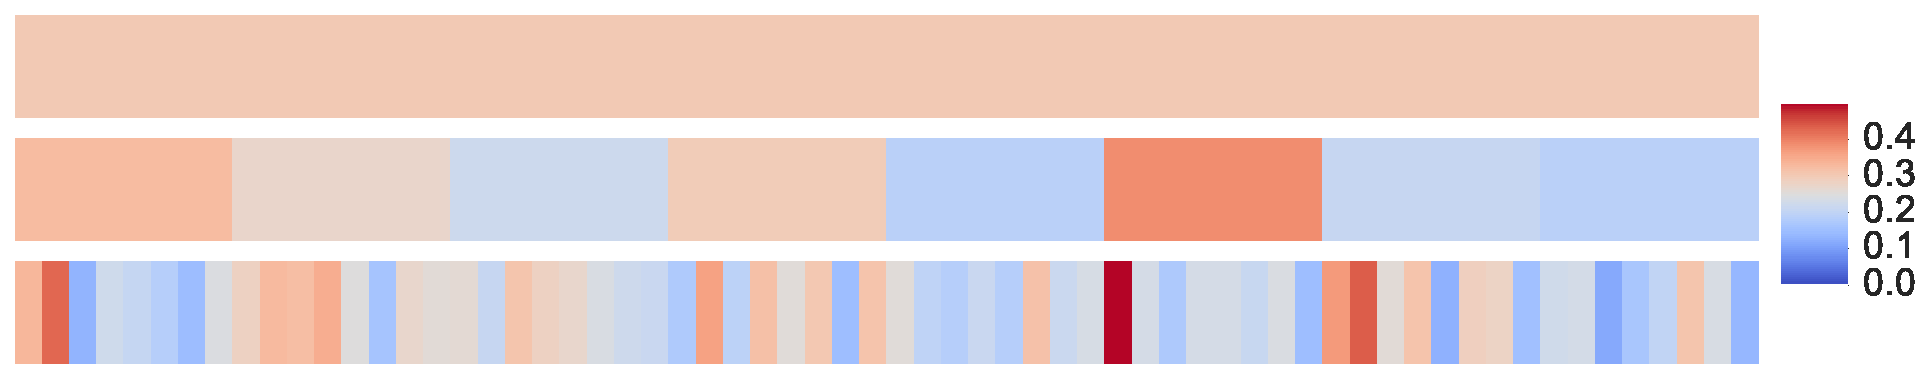
\includegraphics[width=0.6\linewidth]{hmap_dim0_nonorm.pdf}
    \label{fig:cubeHeatmap0}
  \end{subfigure}
    \begin{subfigure}{\textwidth}
    \centering
    \caption{Dimension 1 Heatmap Set}
        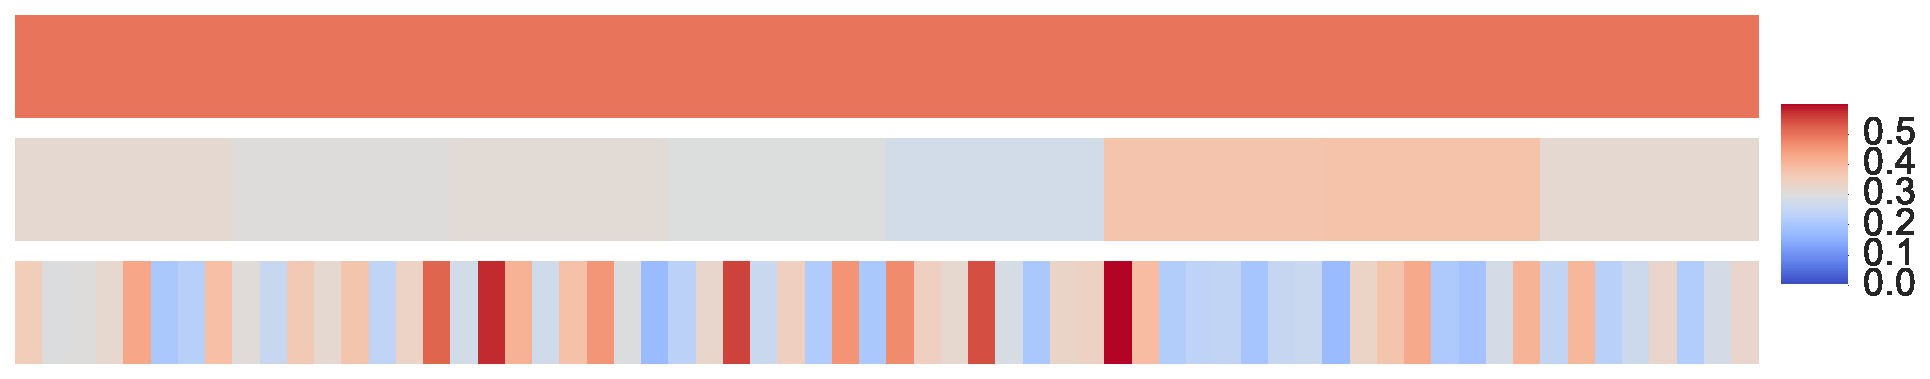
\includegraphics[width=0.6\linewidth]{hmap_dim1_nonorm.pdf}
    \label{fig:cubeHeatmap1}
  \end{subfigure}
    \begin{subfigure}{\textwidth}
    \centering
        \caption{Dimension 2 Heatmap Set}
        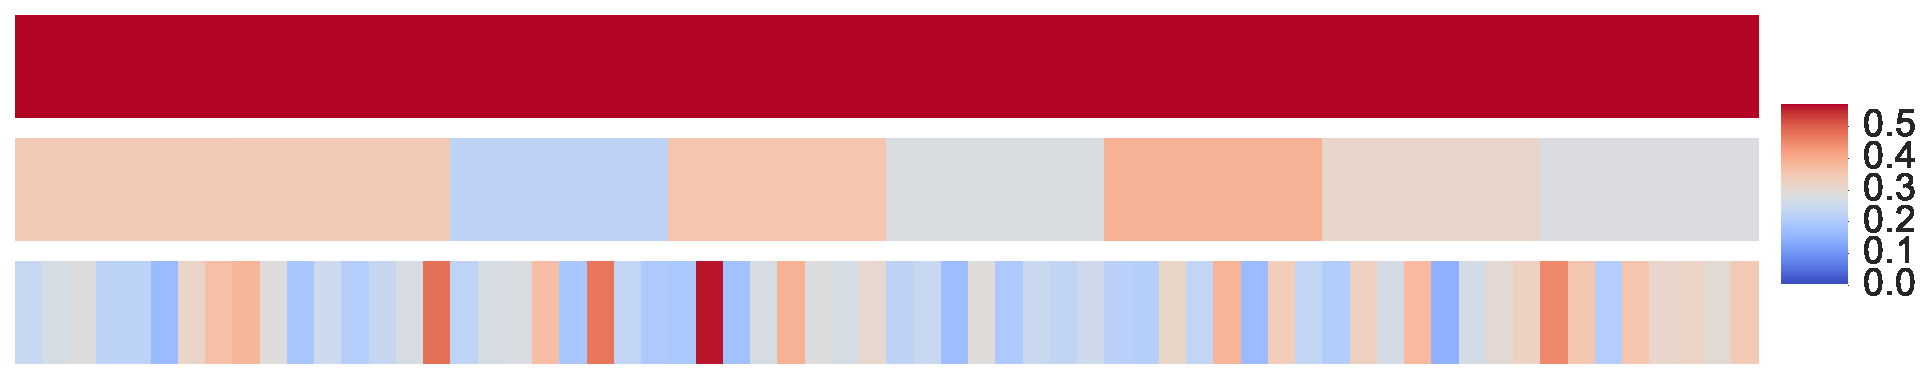
\includegraphics[width=0.6\linewidth]{hmap_dim2_nonorm.pdf}
    \label{fig:cubeHeatmap2}
  \end{subfigure}
    \caption{Each sub-figure contains three horizontal heatmaps respectively representing (from top to bottom) the  Bottleneck distances between each slice of unsplit, double split, and quadruple split pairs from respective WDM and CDM data sets by dimension. Each individual heatmap is a  vectorization of the cubic slices produced from the WDM and CDM Eagle simulations.}
    \label{fig:cubeHeatmap}
\end{figure}

From figure \ref{fig:cubeHeatmap}, we can infer that the topological and geometric differences are certainly not uniform across different sections of the observable Universe. For each of the three homologies, introducing a greater number of splits uncovers greater variance in magnitudes of bottleneck distances between CDM and WDM cubes. This suggests that it's possible for topological differences to be masked by local similarities, and that there exist partitions of topologically similar areas and partitions of topologically different areas within the EAGLE simulation. Further work should explore what areas in the Universe occupy these two partitions and if there exist physical evidence of differences. Provided that the Euler Characteristic Function and the Correlation Function were the two most effective hypothesis tests, to confirm the validity of these heatmaps, we compared these two functions for the cubes with the highest bottleneck distance and the cubes with the lowest bottleneck distance. If valid, we should expect to see greater differences in the functions among the cubes with high bottleneck distance.

\begin{figure}[htp!]
  \centering
    \begin{subfigure}{0.21\textwidth}
    \centering
        \caption{EC (High)}
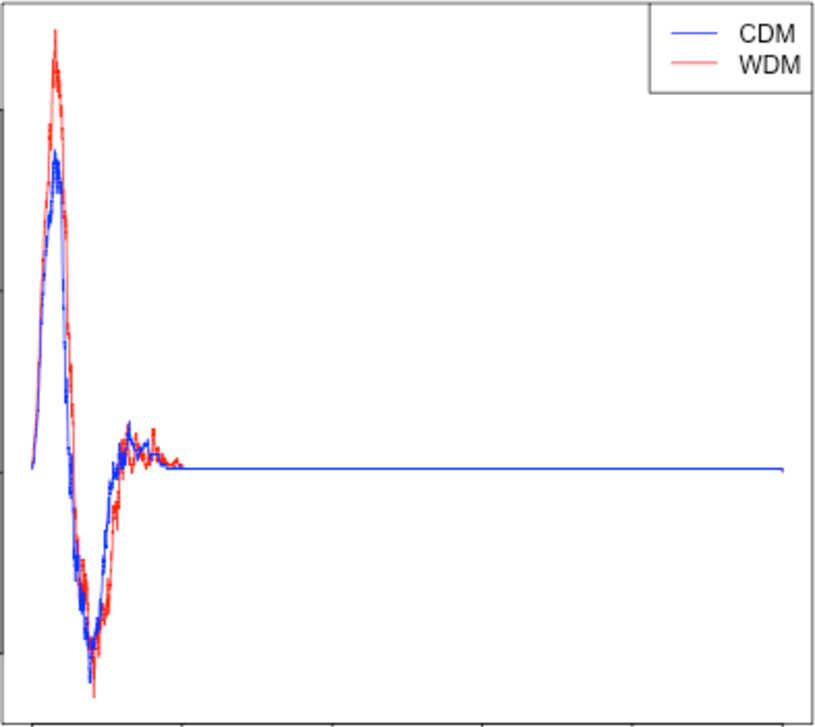
\includegraphics[width=\linewidth]{valid1.pdf}
    \label{fig:valid1}
  \end{subfigure}
    \begin{subfigure}{0.24\textwidth}
    \centering
        \caption{CORR (High)}
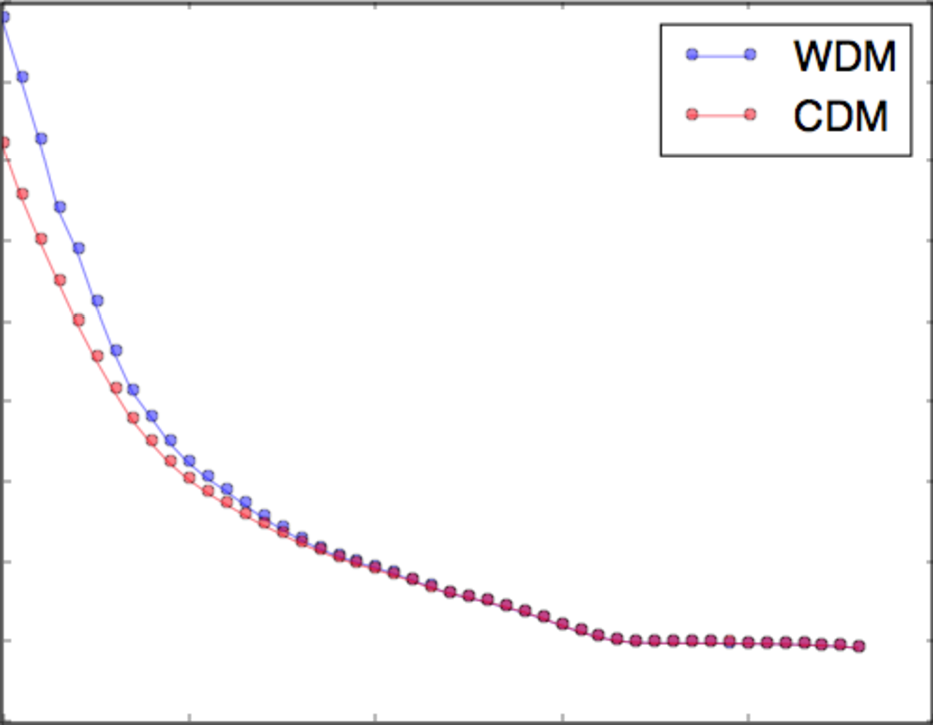
\includegraphics[width=\linewidth]{valid2.pdf}
    \label{fig:valid2}
  \end{subfigure}
    \begin{subfigure}{0.21\textwidth}
    \centering
        \caption{EC (Low)}
\includegraphics[width=\linewidth]{valid3.pdf}
    \label{fig:valid3}
  \end{subfigure}
    \begin{subfigure}{0.24\textwidth}
    \centering
        \caption{CORR (Low)}
\includegraphics[width=\linewidth]{valid4.pdf}
    \label{fig:valid4}
  \end{subfigure}
    \label{fig:validationfigs}
    \caption{A comparison of the Euler Characteristic Function and the Correlation Function for Dimension 1 between the cube with the highest bottleneck distance and the cube with the lowest.}
\end{figure}

As expected, figure ~\ref{fig:validationfigs} confirms that the (High) functions are less similar than the (Low) functions. The same pattern arises for Dimension 0 and Dimension 2.  

\begin{figure}[htp!]
  \centering
    \begin{subfigure}{\textwidth}
    \centering
        \caption{Dimension 0 Standardized Heatmap Set}
        \includegraphics[width=0.6\linewidth]{hmap_dim0_yesnorm.pdf}
    \label{fig:cubeHeatmapStand0}
  \end{subfigure}
    \begin{subfigure}{\textwidth}
    \centering
        \caption{Dimension 1 Standardized Heatmap Set}
        \includegraphics[width=0.6\linewidth]{hmap_dim1_yesnorm.pdf}
    \label{fig:cubeHeatmapStand1}
  \end{subfigure}
    \begin{subfigure}{\textwidth}
    \centering
        \caption{Dimension 2 Standardized Heatmap Set}
        \includegraphics[width=0.6\linewidth]{hmap_dim2_yesnorm.pdf}
    \label{fig:cubeHeatmapStand2}
  \end{subfigure}
    \label{fig:StandCubeHeatmap}
    \caption{Each sub-figure contains three horizontal heatmaps representing Bottleneck distances identical to those shown in figure  \ref{fig:cubeHeatmap} but standardized persistence diagrams were used instead.}
\end{figure}

We can do the same heatmap experiment with the standardized persistence diagrams of the CDM and WDM simulations prior to splitting. As confirmed in the hypothesis testing of both the Voronoi and the EAGLE simulations, standardizing removes geometric differences, greatly reducing the bottleneck distances, as seen in figure  \ref{fig:StandCubeHeatmap}. Notably, for dimensions 0 and 1, the cube with the largest bottleneck distance remained the same as in the unstandardized heatmaps, suggesting that those differences are largely not due to size, but true topological distinctions. Dimension 2, however, was less consistent, possibly indicating that voids in CDM and WDM are more aberrant in terms of size, not topological shape. Despite the differences standardizing induced, we are still confident that differences in topology alone are not uniform across the EAGLE Universe: certain splits are consistently indicating differences in dark matter make-up between warm and cold assumptions.

%%%%%%%%%%%%%%%%%%%%%%%%%%%%%%%%%%%%%%%%%%%%%%%%%%%%%%%
%% SECTION: CONCLUSION
%%%%%%%%%%%%%%%%%%%%%%%%%%%%%%%%%%%%%%%%%%%%%%%%%%%%%%%

\section{Conclusion}
\label{sec:conc}
In this paper, we presented a hypothesis testing framework, build on persistent homology, to compare topological summaries of two sets of point cloud data. We showed empirically that such a framework is able to infer differences in the true distribution of topology by comparing Voronoi tessellations with controlled hyperparameters. Additionally, we presented the application of this framework on the EAGLE data set to analyze the topology of the cosmic mass given assumptions of warm and cold dark matter, resulting in the discovering of locally significant spatial differences in geometry and topology, and the distinction between the two. We believe this framework may provide a standard method for evaluating hypothesis regarding topology in a diverse array of fields that greatly improve over currently existing methods. 

%%%%%%%%%%%%%%%%%%%%%%%%%%%%%%%%%%%%%%%%%%%%%%%%%%%%%%%
%% SECTION: SUPPLEMENTS
%%%%%%%%%%%%%%%%%%%%%%%%%%%%%%%%%%%%%%%%%%%%%%%%%%%%%%%

\bigskip
\begin{center}
{\large\bf SUPPLEMENTARY MATERIAL}
\end{center}

\begin{description}

\item[Title:] Brief description. (file type)

\item[R-package for  MYNEW routine:] R-package �MYNEW� containing code to perform the diagnostic methods described in the article. The package also contains all datasets used as examples in the article. (GNU zipped tar file)

\item[HIV data set:] Data set used in the illustration of MYNEW method in Section~ 3.2. (.txt file)

\end{description}

%%%%%%%%%%%%%%%%%%%%%%%%%%%%%%%%%%%%%%%%%%%%%%%%%%%%%%%
%% SECTION: REFERENCES
%%%%%%%%%%%%%%%%%%%%%%%%%%%%%%%%%%%%%%%%%%%%%%%%%%%%%%%

\bibliographystyle{agsm}
\bibliography{mybib}
\end{document}
